\documentclass[a4paper,12pt,twoside]{book}
\usepackage[utf8]{inputenc}
\usepackage[english]{babel}
%\usepackage{fontspec}
%\setmainfont[
%  Ligatures=TeX,
%  Extension=.otf,
%  BoldFont=cmunbx,
%  ItalicFont=cmunti,
%  BoldItalicFont=cmunbi,
%  SlantedFont=cmunsl
%]{cmunrm}

%\usepackage{polyglossia}
%\setmainlanguage{spanish}

\usepackage[c5paper]{geometry}
%\geometry{inner=2.5cm,outer=2.5cm,bmargin=3.2cm}
%\usepackage[DIV=14,BCOR=2mm,headinclude=true,footinclude=false]{typearea}

%\usepackage{ulem} %Hace que \emph sea subrayar

%\usepackage[p,osf]{scholax}
%% T1 and textcomp are loaded by package. Change that here, if you want
%% load sans and typewriter packages here, if needed

\usepackage{ebgaramond}
%\usepackage[type1]{libertine} % Linux Libertine for zweispaltige Texte
%\usepackage{textcomp}% Required to get special symbols
\usepackage[scaled=.8]{DejaVuSansMono}% FiraMono Typewriter font
\usepackage{PTSansNarrow} 
%\gilliuscondensed
%\usepackage[sfdefault]{FiraSans}
%\usepackage{bm}% Extra bold faces
%\usepackage[lf]{carlito}

\usepackage{lettrine} %Capital letters at the beginning of a chapter
\usepackage[activate={true,nocompatibility},final,tracking=true,kerning=true,spacing=true,factor=1100,stretch=10,shrink=10]{microtype}
\SetTracking{encoding={*}, shape=sc}{-20} % versalitas menos separadas
% activate={true,nocompatibility} - activate protrusion and expansion
% final - enable microtype; use "draft" to disable
% tracking=true, kerning=true, spacing=true - activate these techniques
% factor=1100 - add 10% to the protrusion amount (default is 1000)
% stretch=10, shrink=10 - reduce stretchability/shrinkability (default is 20/20)

%\usepackage{array,multirow,booktabs,colortbl,chngcntr} % El último es para counterwithout;
\usepackage[strict]{changepage}
%\usepackage{caption}
%\captionsetup{format=plain,labelsep=newline,labelfont={small,sc},
%textfont={small,it},singlelinecheck=false}
\usepackage[Bjornstrup]{fncychap} % Para cabeceras de capítulos sofisticados:     Sonny,    Lenny,    Glenn,    Conny,    Rejne,    and Bjarne.

\usepackage{graphicx,wrapfig,booktabs,multicol} % wallpaper: poner imágenes de fondo; wrapfigure: figuras a un lado del texto
%\graphicspath{{figures/}}
\usepackage{fancyhdr}
\usepackage{emptypage,pdfpages,fancybox} % Para que las páginas en blanco no tengan encabezado;
\usepackage{enumitem} %paralist: para compactenum, enumerate sin espacios
%\setlist[itemize]{nosep} %Espacio entre items en itemize
\usepackage[hyperref]{xcolor}
\usepackage[hidelinks]{hyperref}
\usepackage{xurl}

%\usepackage{minipage}

%\usepackage{quotchap} %Encabezados de capítulos
\usepackage{syntonly,verbatim}
%\syntaxonly

\usepackage{setspace,xspace} % xspace: Da \xspace para no tener que poner {} después de los comandos; pdflscape: páginas en horizontal;

\newenvironment{quotex}{\begin{quote}\small}{\end{quote}}
\newenvironment{quotationx}{\begin{quotation}\small}{\end{quotation}}


\begin{document}

% Por alguna razón, los marginados se creaban al revés. Así los corrijo. Feo, pero eficaz:
\let\tmp\oddsidemargin
\let\oddsidemargin\evensidemargin
\let\evensidemargin\tmp
\reversemarginpar

%\setcounter{secnumdepth}{4} % Para que llegue a numerar hasta las subsubsecciones;
%\renewcommand{\heavyrulewidth}{0.14em} % Grosor de las líneas extremas de las tablas;
%\renewcommand\thempfootnote{\alpha{mpfootnote}} % Símbolo de notas dentro de minipage
%\let\oldcaptionof\captionof
%\renewcommand{\captionof}[2]{\oldcaptionof{#1}{\newline \textit{#2} }}
%\renewcommand{\tablename}{Tabla}
%\counterwithout{figure}{chapter}
%\counterwithout{table}{chapter} % Así la numeración es 1, 2, 3... y no 1.1, 1.2... y no reinicia la num. en cada capítulo;

%\providecommand{\ggl}{\guillemotleft}
%\providecommand{\ggr}{\guillemotright\xspace}
\providecommand{\flright}[1]{\begin{flushright}#1\end{flushright}}
\providecommand{\flrightit}[1]{\begin{flushright}\itshape #1\end{flushright}}
%\renewcommand\UrlFont\sffamily
\urlstyle{tt}

\pagestyle{fancy}
\renewcommand{\sectionmark}[1]{\markright{#1}}
\renewcommand{\chaptermark}[1]{\markboth{#1}{}}

%Portada:
%\includepdf{00Portada}

\frontmatter
%
%\onehalfspacing
%\pagenumbering{Roman} %gobble es como empty

%\include{preindice}

%\fancyhf{}
%\fancyhead[LE]{\small \textbf{\thepage}$\quad$ Índice general}
%\fancyhead[RO]{\small Índice general $\quad$\textbf{\thepage}}
%\clearpage
\tableofcontents

%\doublespacing
\mainmatter

\fancyhf{}
\fancyhead[LE]{\small \thepage$\quad${\scshape\chaptername{} \thechapter}: \nouppercase{\itshape\leftmark}}
\fancyhead[RO]{\small \textsc{Section }\thesection{}: \nouppercase{\itshape\rightmark} $\quad$\upshape\thepage}
%\cfoot{\bfseries\thepage}

\pagenumbering{arabic}

%\onehalfspacing

% introductorios

\chapter{Introduction}
\section{Excerpt from Forming the Soul}

\begin{quotex}
The following is an excerpt from a tract circulated within the \emph{Orthodox Word}; it was written by the Sisters of St. Xenia's Skete. A good friend of mine gave it to me a long while ago.

There is food for thought here, as the writer(s) argue that old Western culture can be a sort of \emph{pre-evangelium} to form the soul in preparation for higher spiritual discipline. I find it interesting on the grounds that the Orthodox Church is officially strongly anti-Western (at least theologically) \& that the argument here is a case of sophisticated and wise application of difficult doctrines which the body of Christians ordinarily use to ignorantly argue against “higher learning”.

\end{quotex}
To regard everything Western as immediately suspect argues a profound insecurity, a \emph{legalism} more rigid than any sect, a scholasticism more arid than any \emph{summa}. We have not inherited Western culture at all. That is precisely our trouble. We have simply grown up on the degenerate and decaying vestiges of that culture. We live, not in the West, but on the fading memory of the West. Our present culture is an absence of culture, a vacuum that has left our souls shrunken and our spirits stifled. Before trying to plunge his spirit into the deeps of Orthodoxy, today's man must first feed his soul, for its paucity will not permit any profound growth of spirit. Modern Western man is like a plant with the shallowest of possible roots, and he naturally cannot support any great growth. His spirit is no longer capable of soaring, because a lofty spirit must rise out of a deep soul which has the maturity, the sensitivity, to feel noble things and become ennobled by them.

Without this, it is difficult to attain sobriety, fruitfulness, authenticity, depth, in our spiritual lives, simply because an unformed, uncultivated, undisciplined soul seldom has the discernment and balance to see clearly and honestly, nor the sensitivity to feel deeply, nor the intensity to strive wholeheartedly, nor the idealism to reach uncompromisingly for what is truest and best. This capacity of the soul is not in and of itself spiritual. Rather, it serves as a preliminary to spiritual things, and it acts as a sort of spiritual tuning fork, often helpful in preserving a well-grounded, sober, discriminating, yet exalted habit of mind. It will be both restraint and prod. We must regain the capacity of soul which can only be developed by proper and careful cultivation.

It is psychologically impossible for us suddenly to become “non-Western”, even if such a thing was desirable. It is spiritually unwise to try to feed a spirit from a dead and dormant soul, and it is intellectually irresponsible to offhandedly reject the treasures of hundreds of years of Christian culture in hopes of escaping the taint of Westernism. If we reuse to nourish ourselves on what is edifying and elevating, we will inevitably be fed by what is not, as the popular culture of America, in all its shallowness and falseness, seeps into our unguarded hearts daily. If we do not counteract it, if we fail to set the loftiest things before us, we will inevitably let our souls remain choked with artificiality and cheapness. We will remain mired in the fatal shoddiness of world and ourselves, and we shall not be able to touch the depths of our own hearts, nor answer the needs of our neighbor's.

The Orthodox Christian who wishes to avoid crippling even further the already spiritually-underdeveloped soul of today's man can find his guide in the actions of the early Church, and he can also find there his defense against those who would wish to regard all artistic and intellectual pursuits as worldly or useless. When the Church denounced pagan culture, She denounced only those aspects of it which were based on or nourished by the demonism of pagan religion or the hedonism of pagan art. Those aspects of Hellenic culture which were useful and healthy, She not only refrained from denouncing, but even transmuted into a profoundly convincing missionary statement. Then, as now, many decried the use of secular art and learning as a means of cultivating and educating the soul, defending their position with the Apostle's warning to \emph{beware lest any man spoil you through philosophy and vain deceit, after the traditions of men, after the rudiments of this world, and not after Christ} (Col. 2:8). In answering them, the Fathers of the Church formulated the response which has remained the Orthodox position on the issue, a response expressed in the teachings of men such as Clement of Alexandria, St. Basil, \& St. John Damascene.

In his \emph{Stromateis}\footnote{\url{http://www.newadvent.org/fathers/0210.htm}}, Clement teaches that the Apostle's warning applies only to those who have turned back from spiritual things to the things of the world, from the ultimate truth of Christ to the partial truth of secular learning, “philosophy being most rudimentary compared to Christianity, and only a preparatory training for the truth” (\emph{Strom}, VI, 7).

It is quite true that the study of poetry, history, art, fiction, is indeed a “most rudimentary” one. It is indeed not a spiritual study. But we, in our modern condition, are in dire need of the rudiments, not only of spiritual life, but of simply humanity. It is absolutely imperative for us to elevate our souls before trying to participate in any sort of authentic spiritual life. To try to ignore or to overleap this primary step leads only to spiritual sterility or deception. We do not live in a normal age, and we are no longer normal people, even by the minimal standards universal to previous ages in the lief of fallen man. The Apostle warns us not to mistake the lower life of the soul for the higher life of the spirit, and warns us not to turn back from the fullness of Christ to the emptiness of the world, but he does not tell us to ignore the development of the soul altogether…The Fathers have always taught that the higher, spiritual part of man's nature is founded on the first level of the soul, that which is sensitive to and best developed by the study of virtuous, noble, and beautiful things. Our faculties and responses, distorted by the Fall, must be restored, through virtue, to normalcy, and after that we can begin to progress in spiritual things…

[...]

He treasured hierarchy because it was for him a reminder of God. His whole world was an endlessly unfolding, interlocking allegory of the majesty and love of God. He rejoiced in the delight of obedience and walked fearfully in the humility of command, because both were images of profound spiritual realities. He revelled in the color and beauty of the physical world, because they were fore-shadowings of the even greater splendors of the Kingdom of God. He could spend his entire adult life building a cathedral, and never forget the transcience of the the temporal world.

His whole world acted continuously to form his soul in an elevated way. His literature, didactic and moralistic, reminded him of the beauty of virtue and nobility, and the brevity of life, and his poetry sang of his delight in the created world and his awe of God…His society taught him to feel the reality and proximity of the spiritual realm almost more intensely than the physical. His churches, resplendent, delicate, glowing, lifted his soul on traceries of stone, and set his spirit on the heights.

The spiritual impetus of that world carried over for almost a thousand years more. The nourishment provided by a thousand years of Orthodoxy was the spiritual ground in which grew all the best in Western thought and art, and that impetus remained largely intact until the Enlightenment, was eroded greatly during the Romantic Age, and finally crumbled entirely in our own time. The best that was done, was done in this spirit, springs from this world. The community of feeling and intent which marks the best of our writers, artists, musicians, springs from this source. Regardless of social, political, and religious changes, Shakespeare and Dickens, Bach and Mozart, Donne and Hugo share the same world, and it is to this world the Orthodox Christians of today must look for formation of soul. There are lessons we must learn from our own past before we can possibly hope to go on.

We must recover the feelings and sensitivities which were once the common property of all civilized people. Those works of art, of literature, of music, which are pre-modern are of essential value for us. They can teach us, as will nothing we ourselves now produce, what nobility is, what virtue is, what honor and purity are, what sacrifice and loyalty are, what is worthy and what is not. Poetry, music, art, fiction, are not spiritual food, but are rather the milk and bread we need to strengthen ourselves to live on the meat of the spirit.



\flrightit{Posted on 2012-10-05 by Logres }

\begin{center}* * *\end{center}

\begin{footnotesize}\begin{sffamily}

\texttt{william zeitler\footnote{\url{http://www.williamzeitler.com/}} on 2012-11-03 at 11:28 said: }

“He treasured hierarchy…” Who is the `he' to whom this blog refers?



\texttt{Logres on 2012-11-03 at 14:35 said: }

The average peasant, who had a finer sense of what is actually real than 90\% of our America. Listening to Americans reminds me of those old movies where the mayor comes out to say a “few words” about the community, which invariably ends up being the “best”, “finest”, “happiest”, etc., etc. in all kinds of ways, in the world. And I am an American. Why are we this way? I think I have a few clues…


\hfill


\end{sffamily}\end{footnotesize}

\section{Graduation Day}

Here are some suggested spiritual practices and how to know when success is achieved.

\paragraph{Detachment and Spiritual Combat}
The fundamental bases of our esoteric practice are detachment and spiritual combat. A sense of detachment needs to be developed. That is, you become the observer of your own life. You watch yourself make coffee, you watch yourself shave. Whenever you can, you wake up and observe.

In spiritual combat, you guard against the thoughts that enter your mind. You don't control what thoughts arise and when, but you do have some measure of control over what thoughts and images you allow to take root in your mind. If you are not diligent, then they can become obsessions, making it more difficult to root them out.

\paragraph{Intentional Suffering}
You must be willing to make sacrifices when necessary. The first thing to sacrifice is negativity. Yes, people love their negativity and are reluctant to give it up.

Suffering out of love is of a different character. If you give up your meal so your child does not go hungry, your pain turns to joy as you see his hunger satisfied.

Abstinence is the intentional denial of certain beneficial foods for a higher purpose. A common one is to give up meat. We see that in the story of Cain and Abel. Ask yourself what they had for dinner.

Cain had a loaf of bread, since that is all he had. Abel also ate a loaf of bread because he had sacrificed his meat earlier. That is why Abel's sacrifice was accepted; Cain didn't really sacrifice anything.

Purgatory is often misunderstood as a form of punishment. Rather it is a purification, because that process was neglected on earth. According to St. Catherine of Genoa, the souls in purgatory are happy because they know they are doing God's will.

\paragraph{The Persona and Conscious Acting}
The soul life contains many persona, which are the roles we play in our family and social lives. As such, they are necessary. However, there is a problem when the Ego starts identifying with one of those roles, or Persona. We need to be aware of the roles we play. Eventually, you can start playing them consciously and deliberately.

\paragraph{Collective Unconscious}
The task of individuation is achieved when there is harmony and equilibrium between the spontaneity of the unconscious and deliberate action by the conscious Ego. To maintain this equilibrium, unconscious processes compensate for the conscious ego to balance the psyche as a whole. These unconscious processes will correct for the egotistical bundle of personal wishes, fears, hopes, and ambitions. However, self-knowledge will ameliorate the effects of these processes, which manifest as irrational and uncontrollable impulses. As consciousness is widened, the actions of the ego will be freed from these unconscious corrections.

Clearing away the fog of this personal unconscious will reveal a deeper layer, called the collective unconscious. Man's mind is not a blank slate. Rather, the common heritage of the human race is contained in the mind as archetypes, which manifest themselves endlessly in history. Jung gives as examples the parent archetype, which is the reflection of the parent in the child. Of course, the collective imago is intertwined with a personal imago, since the child cannot fully understand the parent. There is also the imago of the child itself. This allows for the spontaneity of play. One can become child-like in this regard, which is not at all the same as being childish.

A man will have an interior image of a woman (anima) and a woman, that of a man (animus). The Sage is another one, since everyone tries to be wise to some extent in his own life. The human mind is prepared for psychic life just as the body is prepared for material life. It is inborn in him. Jung writes about it:

\begin{quotex}
The whole nature of man presupposes woman, both physically and spiritually. His system is tuned in to woman from the start, just as it is prepared for a quite definite world where there is water, light, air, salt, carbohydrates, etc. The form of the world into which he is born is already inborn in him as a virtual image. Likewise parents, wife, children, birth, and death are inborn in him as virtual images, psychic aptitudes. These a prior categories have by nature a collective character; they are images of parents, wife, and children in general, and are not individual predestinations. … They are in a sense the deposits of all our ancestral experiences, but they are not the experiences themselves. 

\end{quotex}
\paragraph{Psychology and Esoterism}
When Jung writes as a scientist, he must necessarily limit himself to the phenomena of psychic (i.e., psychological) events. Whether there is something beyond the phenomena is opaque to the scientific method.

On the other hand, the esoterist is definitely interested in what is beyond the merely psychic layer of life. Now Jung in his personal life did indeed believe in the reality of a noumenal reality beyond phenomena. Nevertheless, we are less interested in his spiritual writings, but his immense psychological knowledge can be used profitably.

\paragraph{Megalomania}
There are two main obstacles to spiritual development: the tendency to megalomania and sexual obsession. The former manifests as an unjustified high opinion of oneself. Jung write about several such cases. Such an individual will underrate, belittle, or criticize others, especially those close to him. He shows how unconscious processes will compensate for those feelings.

However, on our path, we don't rely on such unconscious processes. Rather, our method is deliberate and conscious. We notice that this megalomania manifests as “taking accounts”, that is, we are keeping track of all the alleged snubs and mistreatments we have received from others. By observing this tendency in a detached way, the Self will compensate consciously and we make find that such feelings simply dissipate.

It is necessary to “wake up” somehow in order to catch such manifestations “in the bud” as it were, before they can catch hold.

\paragraph{Song of Innocence}
It is accepted that childhood is a time of innocence free from overt, \emph{pace} Freud, sexual thoughts. This is followed by the time of experience. Once again, the notion that sexual activity in itself is somehow bad needs to be dispelled. Rather the issue is the misuse, or better said, the reuse of sexual energy. After the son of duty, different options present themselves. Like the faster, one can give up sex as a form of deliberate suffering, not because it is bad.

The goal is self-mastery, but it soon becomes clear that the desire is quite intense. It doesn't suffice not to engage in sex, because once the idea of it comes into the mind, it will recur, usually in an even stronger way. So it is really a spiritual rather than a material battle. It is a matter of guarding the thoughts.

Perhaps one can remain in the state of innocence for an hour, for a day, even for several days. One becomes a child again, spontaneous and innocent. You stop looking at women with that leering look; you know what that feels like.

Freud wrote of the state of polymorphous perversity, in which sexual energy is not confined to the genital region. The entire body can be on edge. Sometimes it can be difficult to even look at a pretty woman, because the body feels so intense; you may need to shield your eyes in that case.

Often, you just feel really good all day long.

\paragraph{Anima}
The imago of a woman in a man is called the Anima. Jung describes it:

\begin{quotex}
Woman, with her very dissimilar psychology, is and always has been a source of information about things for which a man has no eyes. She can be his inspiration; her intuitive capacity, often superior to man's, can give him timely warning, and her feeling, always directed towards the personal, can show him ways which his own less personally accented feeling would never have discovered. 

\end{quotex}
I want to focus on the esoteric teaching rather than the psychological, although they are compatible. Originally the human being was whole, but such as we are (speaking from a man's point of view), there is a gap in consciousness where the woman belongs. There is one, and only one, who fits perfectly. She may not be found, so there are others who fit less perfectly; some are closer than others.

The two who find each other are called Polar Beings. From an experiential point of view, it suddenly seems as though another person is sharing the same body. Her thoughts become mixed up with your own thoughts, her feelings are your feelings. Times of separation are an ache, times together a joy.

There are states beyond this one, provided certain tests of purity are met. I don't know those states personally, so I'll hold off for now.

\paragraph{Self}
The end result of individuation is the birth of a Self, or Real I, beyond the conscious Ego. The Self is not scientific because it can never be an object of thought. It is noumenal and beyond the psyche. It includes the Ego as well as all the unconscious processes. However, the Self integrates them all into a whole, eliminating the multiple independent little selves that seem to exist.

From the psychological point of view, Jung claims that the experience of the Self and the experience of God are the same.

St. Catherine of Genoa goes beyond that when she writes:

\begin{quotex}
My Being is God, not by some simple participation but by a true transformation of my Being. 

\end{quotex}
\paragraph{Graduation Day}
Quite some time ago, I had been participating in a group for a few years. I noticed the repetitive nature of it and no one seemed to be progressing. There were the same stammerings, the same excuses, the same struggles. One woman expressed the joy she felt communing with the squirrels in the morning.

I suspected most were lying, because my descriptions of the inner life were more vivid — and shocking — than theirs. I had assumed that the two group leaders were following some special program. I learned later that they were just winging it. Moreover, once you moved beyond their own limited frame of reference, they sounded lost. And there was no metaphysical teaching sustaining it.

Not that it wasn't helpful to me, just the opposite. One night I asked the group leader, “When do we graduate?” His response was simple, “Just graduate,” he replied. So I never went back after that.

You graduate when the burden becomes light, as St. Catherine described. You have achieved more self-awareness. You are liberating yourself from the lower forces that enthrall you with anxiety, despair, worry, uncertainty, obsessions. There is no need for any of that.



\flrightit{Posted on 2018-05-04 by Cologero }

\begin{center}* * *\end{center}

\begin{footnotesize}\begin{sffamily}



\texttt{Lyon on 2018-05-06 at 16:10 said: }

This was brilliant on many levels. Thank you! 

One question for you…

You mentioned Freud in your post. My surface-level take on him is that he is a charlatan of the highest order and that his ideas are deleterious. What is your general assessment of him? Apologies if your explicit views on Freud have already been covered in your writings. I am a rather recent visitor to this site.

And a comment…

The St, Catherine of Genoa quotes were profound and sublime. The insights in her quoted words, used judiciously in your post, I found both deeply rooted and uplifting. I never heard of her before visiting this site (…I recalled you mentioning her previously in a post, so at the time I did a quick internet search of her; I will go back to read up on her further).

Thanks again!


\hfill

\texttt{Dennis on 2018-05-08 at 15:12 said: }

My problem isn't getting to “graduation day”, but knowing where to begin the journey properly in the first place in order to even chart a path to “graduation day.” There are just so many books, resources (such as this blog – which itself would take forever to read and digest systematically from beginning to end), etc., that just knowing where to begin and how to separate the wheat from the chaff, so to speak, is daunting. I find myself often flitting from one book to the next, one thinker to the next, with no clear plan or goal, and in a rush of enthusiasms that soon fade, then I move on, hoping the next book or thinker will be the that changes everything for me…and on and on… Any ideas or recommendations from anyone on where and how best to begin?


\hfill

\texttt{F on 2018-05-10 at 09:29 said: }

With the right desire the Bhagavad Gita and Boehmes Way to Christ should be enough to get you started.


\hfill

\texttt{Sean on 2018-05-11 at 12:29 said: }

Not sure how to reply to someone but this is for Dennis.

Dont worry about reading the right books. Start with simple actions in your daily life. I'll give 5 I started with. 

1. Make your bed every day

2. Do some physical activity, a walk, a few push-ups, anything. No need to go to the gym if it feels daunting.

3. Quit all drugs/drinking save special occasions like wine at a wedding.

4. Sacrifice some sort of food. I started with processed carbs and made my way to all meat except wild caught fish. (still have difficulty with sugar)

5. Think positive thoughts about all you people you encounter. It's easy to judge that obese lady who buys nothing but Pepsi at Walmart but try and only let yourself think something positive about her. Even if you can't confirm it. Sometimes I'll think “I bet she's a really great aunt” or something.


\hfill

\texttt{lenamaria5 on 2018-05-15 at 19:36 said: }

@Dennis, Sean gave some good suggestions. I have also struggled with flitting from book to book. Perhaps that's a product of my (our?) generation's digital consumption habits and general lack of focus. It is much better to concentrate one's efforts on a single work or thinker for a longer period, aiming for depth and not breadth. Read meditatively, rather than just seeking information. Set a much longer timeline than you think you need for a work. If you've read through it before the time is up, you've read too quickly. Gornahoor has a post on Lectio Divina that's very good, if you're interested in Holy Scripture.


\end{sffamily}\end{footnotesize}

\section{Rules too Difficult for Young Men}

The Internet has been able to create a new type of Star. The iSoapbox has given non-standard viewpoints a small space in which to be heard. There are the pretty right-wing girls who do well. However, men also gain larger audiences.

Recently a Star was born in the persona of a Canadian psychologist, and his influence has extended beyond the confines of the Internet. Part of his appeal, it has been said, is that he provides a positive message to young men. That may be true, even if the necessity for it is sad.

Once in a while, someone suggests to Cologero that he should be on TV. I'm sure they intend that as a sort of praise, although they have really not thought things through. First of all, the message here is a bit too difficult to summarize. The professor's worldview, on the other hand, can be summarized in a paragraph or perhaps in 12 rules for life. Then it is a matter of repetition.

Also — and I can say this — Cologero does not have a very dynamic personality. Not experiencing emotions like most of the world, he cannot imitate that pained, thoughtful look, nor does he weep on cue. Furthermore, he is quite low on “amiability”. He eschews current events and does not believe in “debates”.

Nevertheless, Gornahoor has touched on many of the same themes to a much smaller audience. These rules for life have been available online for several years with minimal impact. While Cologero is preoccupied, I've taken the liberty to propose Gornahoor's rules for life for young men. There must be some who can handle a deeper understanding of Life.

\paragraph{Stand up straight}
Those who have participated in the online seminars would have heard of the importance of posture since the very first meeting. Cologero has recommended the Alexander technique for those who still have trouble. Moreover, posture is just one aspect of a larger theme which includes voice, intonation, facial expression, and so on. Mastery of the body is part of self-development.

In a larger perspective, this includes physiognomy which includes more than just a face. Curiously, once out of favor, scientific interest in physiognomy has been growing.

\paragraph{Hierarchy}
\begin{quotex}
The authors of the Middle Ages could not imagine … the Universal Church without a pope. Because if the world is governed hierarchically, Christianity or the \emph{Sanctum Imperium} cannot be otherwise. Hierarchy is a pyramid which exists only when it is complete. \flright{\textsc{Valentin Tomberg}, \emph{Meditations on the Tarot}}

\end{quotex}
It is one thing to joke about the hierarchy of lobsters, but quite another to follow the hierarchy created by God. There is no need to repeat the details here, since the notion can be found throughout Gornahoor. There can be no compromise. It can be a difficult teaching because few want to accept voluntarily their rightful place in any hierarchy.

\begin{quotex}
A pyramid is not complete without its summit; hierarchy does not exist when it is incomplete. Without an Emperor, there will be, sooner or later, no more kings. When there are no kings, there will be, sooner or later, no more nobility. When there is no more nobility, there will be. Sooner or later, no more bourgeoisie or peasants. This is how one arrives at the dictatorship of the proletariat, the class hostile to the hierarchical principle, which latter, however, is the reflection of divine order. This is why the proletariat professes atheism. \flright{\textsc{Valentin Tomberg}, \emph{Meditations on the Tarot}}

\end{quotex}
\paragraph{Purification}
This is the metaphysical equivalent to “clean your room”. Granting that as a metaphor for “get you own life in order”, that is not possible without first getting your inner life in order. Here are some links to get you started.

\begin{itemize}
\item Purification of the Will\footnote{\url{https://www.gornahoor.net/?p=6950}}
\item Purity of the Mind\footnote{\url{https://www.gornahoor.net/?p=6961}}
\item Purification of the Word\footnote{\url{https://www.gornahoor.net/?p=6969}}
\item Purification of the Sex Act\footnote{\url{https://www.gornahoor.net/?p=6985}}
\item Purification of the Breath\footnote{\url{https://www.gornahoor.net/?p=6991}}
\item Moral purification of the Will\footnote{\url{https://www.meditationsonthetarot.com/moral-purification-of-the-will}}
\end{itemize}
\subsection*{Self-Mastery}
Self-mastery or autarchy is:

\begin{quotex}
For those who have absolutely possessed themselves, the alogon indicates only the unconditionality of his will, autarchy. Therefore, beyond the abstract intellectual, there is still an abyss between the man who lives his own life as lord and master, and the man who feels himself only as a demonic force of a nature that is passive to himself and that has its raison d'être outside himself. 

\end{quotex}
First, the autarch must master his thoughts, then his emotions, and ultimately his body insofar as it is possible. This is actually the Hermetic path, since each of those stages of self-mastery leads to the development of higher states of being.

\paragraph{Learn a martial art}
If so inclined, learn a martial art or become skilled in weaponry. A martial art develops concentration and attentiveness. The competition simulates life and death situations. Cologero wrote:

\begin{quotex}
A man, for his preparation, can conquer his fear of the elements: fire, air, water, and earth. Overcoming such fears leads to self-knowledge and a concentrated mind. Those with a warrior cast of mind need to excel at a martial art or develop skill with weaponry. Time spent in this way is more beneficial than excessive, or obsessive, reading. If you don't regard these activities as spiritual, then make them so. Do them with the right attitude and full consciousness. 

\end{quotex}
\paragraph{Spiritual Combat}
Spiritual combat is the analog of martial arts on a higher plane. However, at this level one's eternal life is at stake.

\begin{quotex}
Even without being killed a man can experience death, he can conquer, he can realize the culmination characteristic of a “super-life”. From a higher point of view, Paradise, the Kingdom of Heaven, Valhalla, the Island of the Heroes, etc., are only symbolic figurations forged for the masses, figurations that in reality designate transcendent states of consciousness, beyond life and death. The ancient Aryan tradition used the term \emph{jivan-mukti} to indicate such a realization while still in the mortal body. \flright{\textsc{Julius Evola}}

\end{quotex}
\paragraph{The Modern World}
It is necessary to have an adversary relationship to the modern world, even if only private. That means “to be in this world but not of it”. In anticipation of ridiculous comments, “modern” does not simply mean “contemporary”. We are neither Luddites nor Amish. Here are two of three steps (the third is in preparation).

\begin{itemize}
\item Understand the crisis of the Modern World 
\item Revolt against the Modern World 
\end{itemize}
\paragraph{Honor your father}
Honoring your father means gratitude for your inheritance and respect for those ancestors who created it. For Western Europeans, these are the three main currents of that inheritance.

\begin{itemize}
\item Hellenic Culture 
\item Roman Tradition 
\item Neoplatonic philosophy 
\end{itemize}
\textbf{Hellenic Culture}: The Hellenes have given us art, philosophy, political theory, and folk religion. Therefore, either create, or learn to appreciate, poetry, sculpture, drama (both tragedies and comedies). Develop a foundation in the trivium of grammar, logic, rhetoric: learn to speak well, logically, and persuasively. Learn the various types of political systems and the causes of their degeneration.

Pure thought is insufficient. A good life will include the Greek virtues: temperance, prudence, courage, and justice.

The Greek folk religion included reverence of ancestors, respect for the founders, and engaged the whole being in every aspect of life. Hegel describes it this way:

\begin{quotex}
In a folk religion in particular it is of the utmost importance that the imagination and the heart not be left unsatisfied: the imagination must be filled with large and pure images, and the heart roused to feelings of benevolence. 

\end{quotex}
\textbf{Roman Tradition}: The Romans brought us martial valor, administration, and engineering.

The primary Roman virtues included Piety, Gravitas, Dignitas, and either manliness or modesty.

\textbf{Neoplatonic Philosophy}: Neoplatonic philosophy integrated the best parts of Plato, Aristotle, and Stoicism. It is a powerful counterweight to contemporary philosophies of naturalism or materialism. A thinking man should always be an idealist, since the understanding of ideas is the aim of thought.

Start with \textbf{Augustine of Hippo}, \textbf{Dionysius the Areopagite}, and \textbf{Boethius}.

\paragraph{Conclusion}
If you've come this far, then draw your own conclusions.



\flrightit{Posted on 2018-03-17 by Aeneas }

\begin{center}* * *\end{center}

\begin{footnotesize}\begin{sffamily}



\texttt{manfred arcane on 2018-03-18 at 05:53 said: }

I see Peterson as a gateway drug, of sorts, to traditionalism. He is not there of course, not even close, but he is pointing people in the right direction and his lectures – if they bother to follow them – are providing them with tools with which they can approach a number of relevant thinkers. And, given his reach, that is a good thing – even if the 1\% of his followers decide to do a deep dive into Jung or Heidegger thanks to him, and even if the small portion of that 1\% eventually reaches the strain of thought that is espoused by the blogs like this one.


\hfill


\hfill

\texttt{Matt on 2018-03-19 at 08:44 said: }

George Heart, in his book “Christianity: Dogmatic Faith \& Gnostic Vivifying Knowledge” seeks to address the crisis of the lack of faith in modern people, by understanding the root cause, which is revealed in the Law of 3: the active force being the Church, the passive force being man's spirit/Personality, and the equilibrating force (the root of the issue) being change.

What has changed is that modern man has developed a stronger intellect, whereas the Church still preaches a simplistic “milk of the spirit” theology.

Perhaps this Canadian psychologist is gaining a foothold with many of his followers, on topics that don't usually have mass appeal (biblical analysis and hierarchy), partially due to his ability to engage and excite the intellect.

It's also interesting that he has discovered the hierarchical principle in nature, but fails to see it as the reflection of something higher.

http://matthewnanderson.wordpress.com/


\hfill

\texttt{LHOOQ on 2018-03-21 at 07:54 said: }

Manual of Epictetus is a good read to begin an ethical and philosophical life.


\hfill

\texttt{Kenneth Lyon MacNeil on 2018-03-25 at 14:33 said: }

A deep thank you to all who are responsible for the information and insights on this website. 

I will say little else till I do a deep dive into the information on offer here. I do look forward to doing so. 

Much appreciation,

\~{}Lyon


\hfill

\texttt{Robert on 2018-04-07 at 12:13 said: }

There are many traditionalist resonances in Peterson's work, as far as I can see, and he is far from being dismissive of religious belief. Quite the contrary. See, for example:

jordanbpeterson.com/philosophy/on-the-ark-of-the-covenant-the-cathedral-and-the-cross-easter-message-i/

Although I've seen no evidence that he has read Guénon, Schuon, Coomaraswamy or Evola, Eliade seems to have been important for him.


\hfill

\texttt{Bloom on 2021-03-18 at 17:59 said: }

Nice post, a lot of young men were captivated by Jordan Peterson for at least a year or two before moving onto greener pastures. He's a nice tutorial level boss.

Anyways, I want to add a comment on your last bit about the three main currents of Western Tradition. According to Evola, when we look at the Western Warrior Tradition, the three main currents are: Roman, Christian, and Nordic tradition.


\hfill


\end{sffamily}\end{footnotesize}

\section{What must I read to be saved}

January is the open enrollment period for training in self-awareness and concentration. Please read to the bottom for more information. 

\begin{quotex}
What must I do to be saved? \flright{\textsc{Acts 16:30}}

\end{quotex}
In spite of that, I constantly get asked this one question, via all the communications platforms I am on:

\textbf{What must I read to be saved?}

\begin{wrapfigure}{rt}{.3\textwidth}
 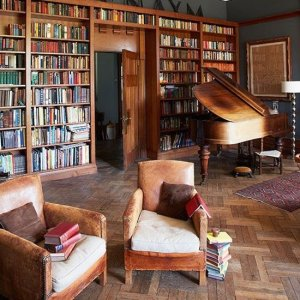
\includegraphics[scale=.4]{a20220102WhatmustIreadtobesaved-img001.jpg} 
\end{wrapfigure}

Reading alone may be necessary for preparation, but it is not sufficient. When I took physics and chemistry classes at university, I had to give up Saturday mornings to do lab work. It wasn't always easy to get up early on weekends, but without the lab work, physics and chemistry are incomplete.

Nevertheless, everyone is looking for the ``magic book". And a month later, they will look for the next magic book because the first one had no effect on them. There is no such book, although many have claimed to benefit from a revealed text like the Bible or the Quran.

I have tried to recommend texts that will provide a firm foundation. Over the years, have I not recommended hundreds of texts by philosophers, poets, metaphysicians, theologians, mystics, scientists, and other thinkers? If you resonate with one or more of them, then read the texts yourself.

\paragraph{Self Study}
If that is not very systematic, then this list by Ananda Coomaraswamy is an excellent resource for self-study:

\begin{quotex}
A European can hardly be said to be adequately prepared for the study of the Vedanta unless he has acquired some knowledge and understanding of at least

\begin{itemize}[nosep]
\item Plato 
\item Philo 
\item Hermes Trismegistus 
\item Plotinus 
\item Gospel of John 
\item Dionysius the Areopagite 
\item Meister Eckhart 
\item Dante 
\end{itemize}

Eckhart, with the possible exception of Dante, can be regarded from an Indian point of view as the greatest of all Europeans. 

\end{quotex}
Carl Jung has a nice list of what he calls the \textit{Ten Pillars of the Bridge of the Spirit}. Even if you believe Jung is a danger or a fraud, the list is still valuable.

\begin{itemize}[nosep]
\item Gilgamesh epic 
\item I Ching 
\item Upanishads 
\item Tao Te Ching 
\item fragments of Heraclitus 
\item Gospel of John 
\item Letters of Paul 
\item Meister Eckhart 
\item Dante 
\item Faust 
\end{itemize}

\phantom{.}

Those two lists of texts will provide a solid grounding in metaphysics. If that is not enough then check out this nice list extracted from Valentin Tomberg:

\begin{itemize}[nosep]
\item Bernard of Clairvaux 
\item Thomas Aquinas 
\item Meister Eckhart 
\item Johannes Tauler 
\item Theologia Germanica 
\item Heinrich Suso 
\item Jan van Ruysbroeck 
\item Nicolas of Cusa 
\item Cornelius Agrippa 
\item Paracelsus 
\item Valentin Weigel 
\item Jacob Boehme 
\item Angelus Silesius 
\item St John of the Cross 
\end{itemize}

\phantom{.}

For a firm foundation of traditional metaphysics, I recommend these books by Rene Guenon:

\begin{itemize}
\item Man and his Becoming according to the Vedanta 
\item Symbolism of the Cross 
\item The Multiple States of the Being 
\end{itemize}
\paragraph{The most privileged men}
Haydar Amuli established the hierarchy of threefold division of thinkers.

\begin{enumerate}
\item The common people or the men of reason 
\item The privileged people or men of intuition 
\item The most privileged people or the men of both reason and intuition 
\end{enumerate}
The lowest level, men of reason, refers to profane philosophy. The middle level refers to mystics, who have the intuition of the Unity of Existence, but not the understanding. Those at the highest level have gnosis; they both know and understand the doctrine.

So where do you want to be in that hierarchy? Or are you content to be among those who have ``gone astray" and don't even bother to get started?

You need to be honest with yourself. How well do you actually read? Can you follow a difficult text? How well did you do on the reading section of standardized tests? You should realize at some point that you need some help to understand these texts.

Do you even understand what is meant by ``intuition"? Are you able to concentrate on an idea for an extended period of time?



\flrightit{Posted on 2022-01-02 by Cologero }

\begin{center}* * *\end{center}

\begin{footnotesize}\begin{sffamily}



\texttt{De Bosit on 2022-01-02 at 04:01 said: }

Beliving in the unity of all and being humble when reading is important.

Just assuming you know instantly… You will just reinforce your existing views.

Cryptic Alchemical texts like Boehmes Signature of All Things will not make sense, but trying to understand, believing there IS something there and pondering passages that stood out to you might get you far.

Also you have to fall in LOVE with what you are doing. It's called philosophy for a reason.

If that spark isn't there, just live your life like you are.


\hfill

\texttt{Santiago on 2022-05-03 at 19:08 said: }

This is a great post, although I believe that it's also appropriate to label and recommend material based on ones own progression. I base the following recommendations largely off of my own errors and mistakes, in the hopes that it might help someone else. 

The writings of Guenon, and to a lesser extent, Evola, are very useful, but they can easily lead a person astray if taken too far, too seriously, or without a broader perspective. In retrospect, I feel one of the largest appeals of those authors is their biting critiques of modernity and their intellectual summary of traditional metaphysics. But these are not enough to present someone with a path (much less a healthy worldview, in some cases) and past a certain point, they may even present an obstacle.

Mouravieff classifies the stages of ones progression as being divided into 3 primary stages (see fig. 56, vol. i of Gnosis): `exoterism’, ‘mesoterism'. and `esoterism' proper. Dividing each stage is a `threshold' which transitions one from one stage to another. Perhaps we should recommend material based on this scheme.

While it might sound strange, perhaps it's best to treat the writings of the `Traditionalists' as being suited almost exclusively to the `exoteric' domain in this progression. Reading them can do very little for ones spiritual work, outside of providing an initial impetus. Alternatively, it might be recommended to concentrate on the Bible, the writings of the saints, church doctors and fathers, etc. for this stage.

After crossing the `first threshold'. reading should take a definitive backseat in favor of personal development. Speaking for myself, this cannot be stressed enough. Mouravieff posits this stage (that of the mesoteric) as being pictorially represented by an ascending case of three stairs. Fittingly, I will recommend to concentrate almost exclusively on three authors for the duration of this stage. The decision is immense because one will spend years upon years in this zone, trying to improve oneself, so the following authors are selected with extreme prejudice.

We can apply a correspondence between the three stairs mentioned above with the traditional understanding of the human personality: that is, of the person composed of intellect, emotion and of bodily will. 

First, I will recommend the writings of Vladimir Solovyov (in particular, Russia and the Universal Church), for it is this book which will present a healthy social outlook, a progressive goal to hope for in the religious and political realm, a great history lesson, a comprehensive metaphysic, and a teleology for all of ones personal efforts along the Way. It is for these reasons that Solovyov can guide the intellect of the the hermetic neophyte.

For development of the heart, it is without a doubt the writings of Valentin Tomberg (and in particular, MOTT) that can serve as a `textbook' guide. The passages of this book should be taken individually, with reading encompassing no more than a few pages at a time. Such is the demand of their emotional and spiritual depth, and they will produce great inspiration.

Lastly, for a program of the will, Mouravieff presents his comprehensive system of interior work and personal development, and plots out every step along an individuals path, and all major points of consideration as regards the readers individual `type'. This is the one author for whom it might be useful to take `notes' as one reads.

After crossing the second threshold, and entering the domain of the esoteric, no reading can be prescribed, as ideally the student would already possess it in spirit.


\end{sffamily}\end{footnotesize}


\chapter{Initiations}
\section{Scire, Potere, Audere, Tacere}

\begin{quotex}
\emph{Scire, Potere, Audere, Tacere}

To know, to be able, to dare, to keep silent

\flright{\textsc{Zoroaster}} 

\end{quotex}

\begin{wrapfigure}{rt}{0.35\textwidth}
\centering
 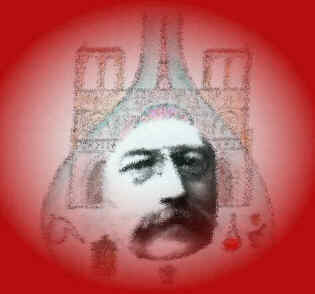
\includegraphics[scale=.25]{a20100928ScirePotereAudereTacere-img001.jpg} 
\end{wrapfigure}

Nature does not open the door of the sanctuary to anyone.

In these pages, the uninitiated will perhaps discover some proof of a genuine and positive science. I do not however, flatter myself that I shall convert them, for I know full well the obstinacy of prejudice and the great strength of preconceived opinions. The disciple will derive greater benefit form this book, provided always that he does not despise the works of the old Philosophers and that he studies with care and penetration the classical text, until he has acquired sufficient perception to understand the obscure points of the practice.

No one may aspire to possess the great secret, if he does not direct his life in accordance with the researches he has undertaken.

It is not enough to be studious, active, and persevering, if one has no firm principles, no solid basis, if immoderate enthusiasm blinds one to reason, if pride overrules judgment, if greed expands before the prospect of a golden future.

The mysterious science requires great precision, accuracy and perspicacity in observing the facts, a healthy, logical and reflective mind, a lively but not over-excitable imagination, a warm and pure heart. It also demands the greatest simplicity and complete indifference with regard to theories, systems and hypotheses, which are generally accepted without question on the testimony of books or the reputation of their authors, it requires its candidates to learn to think more with their own brains and less with those of others. Finally, it insists that they should check the truth of its principles, the knowledge of its doctrine and the practice of its operations from nature, the mother of us all.

By constant exercise of the faculties of observation and reasoning and by meditation, the novice will climb the steps leading to 

\paragraph{Knowledge}
A simple imitation of natural processes, skill combined with ingenuity, the insight born of long experience will secure for him

\paragraph{Power}
Having obtained that, he will still have need of patience, constancy and unshakeable will. Brave and resolute, he will be enabled by the certainty and confidence born of a strong faith, to

\paragraph{Dare}
Finally, when success has crowned so many years of labour, when his desires have been accomplished, the Wise Man, despising the vanities of the world, will draw near to the humble, the disinherited, to all those who work, suffer, struggle and weep here below. As an anonymous and dumb disciple of eternal Nature, he will remain faithful to his vow of silence. In Science, in Goodness, the adept must evermore

\paragraph{Keep Silent}

\flrightit{Posted on 2010-09-28 by Cologero }

\begin{center}* * *\end{center}

\begin{footnotesize}\begin{sffamily}



\texttt{Niko The Exile on 2019-02-15 at 00:18 said: }

This is exceptional, this so much reminds one of the Desert Fathers, i wonder if they were on the same wavelength as Fulcanelli.


\end{sffamily}\end{footnotesize}

\section{Program for Beginners}

\begin{itemize}
\item Furnish your mind as completely as possible with the knowledge of how to inspect and control it. 
\item Train your body to obey your mind, and not to distract its attention. 
\item Control your mind to devote itself wholly to discover your True Will. 
\item Explore the course of that will till you reach its source, your Silent Self. 
\item Unite the conscious will with the True Will, and the conscious ego with the Silent Self. You must be utterly ruthless in discarding any atom of consciousness which is hostile or neutral 
\item Let this work freely from within, but heed not your environment, lest you make difference between one thing and another. Whatever it be, it is to be made one with you by love. 
\end{itemize}

\hfill

References

Crowley, Aleister. \textbf{The Law is for All}



\flrightit{Posted on 2010-09-28 by Aeneas }

\section{Esoteric Training}

This project was conceived some 15 years ago in response to a challenge posed by Rene Guenon: To wit, the recovery of the Western Tradition. As exemplars, there are the civilizations of Medieval Europe and various Eastern Traditions. Hence we endeavored to reinterpret medieval doctrines in the light of Tradition with the aid of the corresponding notions from Oriental Metaphysics.

There are two types of texts: metaphysical and initiatory. Guenon's works are predominantly of the metaphysical type. Specifically, they describe doctrines and ideas in an abstract, impersonal way. Knowledge of doctrine is important, but in itself it is insufficient. It is only potential knowledge.

Initiatory texts are more personal and less explicitly metaphysical, since they describe the pathway from potential knowledge to actual knowledge. Since Guenon mentions Dante's \emph{Divine Comedy} as such an initiatory work, we have used it as the prime exemplar.

So in addition to discursive texts, we have also inaugurated personal training programs without which traditional doctrines are usually incomprehensible. It is usually obvious, when reading about Tradition, which writers have actual knowledge and which do not. What follows is a brief outline of the type of training that might be helpful in lieu of an esoteric school. Strictly speaking, due to individual differences, an initiation is not absolutely necessary, but group work will speed up the process.

Tradition describes the world of Being, essences, the necessary, which alone is fully real. The rest can only see the world of Becoming, the accidental, the contingent.

\paragraph{The Second Birth}
Concentration, meditation, prayer, participating in rite or sacraments, thoughtful reading, and moral purification of the will are preparatory exercises.

Guenon likens initiation to the second birth, aka, being born again. That is at the heart of the Western Tradition, as it was Jesus' nocturnal revelation to Nicodemus. No human individual can make you born again.

\paragraph{Facing the Shadow}
The starting point and ending point are the same, since it is a process: \emph{Know Thyself}.

You will learn exercises to facilitate that process. Initially, the focus is on negativity. Negative emotions, thoughts, and fantasies need to be recognized. The very act of becoming aware of them will attenuate their affects. Nevertheless, few people are willing to confront the Shadow, which is the necessary start to moral purification. Consider these two quotes from anonymous sources:

\emph{Each person has a black mark on his heart when he is born. Once he finds his calling in life, only then does the mark fade away. It is a sin, the sin people hide in their chests. A deep, hidden sin.}

\emph{Find the first truth that terrified you.}

What we fear and what we dislike are more important to self-knowledge than what we love. People reveal what they dislike on the false assumption that it reveals something about the object of their revulsion rather than about themselves.

It is often easier to notice that feature in others than in oneself. People often drop out of group work whenever they come near to discovering their black mark.

\paragraph{Primordial State}
Guenon recognizes three phases on the path to metaphysical realization:

\begin{enumerate}
\item The development of the possibilities of the human state. 
\item The development of supra-individual but conditioned states. 
\item The highest objective is the absolutely unconditioned state, free from all limitation. 
\end{enumerate}
The first step is to create a stable ``I" in the human state. This is Guenon's description:

\begin{quotex}
This realization of the integral individuality is described by all traditions as the restoration of what is called the ``primordial state" which is regarded as man's true estate and which moreover escapes some of the limitations characteristic of the ordinary state, notably that of the temporal condition. The person who attains this ``\textbf{primordial state}" is still only a human individual and is \emph{without effective possession of any supra-individual states}; he is nevertheless freed from time and the apparent succession of things is transformed for him into simultaneity; he consciously possesses a faculty which is unknown to the ordinary man and which one might call the ``sense of eternity." 

\end{quotex}
\subsection*{Supra-human States}
As described in the \emph{Symbolism of the Cross}, we can represent the human state as concentric circles on a plane. In that way we can visualize the first phase as the development of the I at the center. At the center, there is the vertical axis that can be ascended to higher states of being. This is how Guenon describes this phase.

\begin{quotex}
Its second phase corresponds to supra-individual but still conditioned states, though their conditions are quite different from those of the human state. Here, the world of man, previously mentioned, is completely and definitely exceeded. It must also be said that that which is exceeded is the world of forms in its widest meaning, comprising all possible individual states, for form is the common denominator of all these states; it is that which determines individuality as such. The being, which can no longer be called human, has henceforth left the ``flow of forms". 

\end{quotex}
In the \emph{Divine Comedy}, these states are represented by the angelic hierarchies up to the Primum Mobile.

\paragraph{Metaphysical Realization}
Ultimately, there is the Empyrean, which is beyond the conditions of time and space.

\begin{quotex}
The final goal of metaphysical realization; this end remains outside being and by comparison with it everything else is only a preparatory step. The highest objective is the absolutely unconditioned state, free from all limitation; for this reason it is completely inexpressible, and all that one can say of it must be conveyed in negative terms … The only things which have disappeared are the limiting conditions, which are negative, since they represent no more than a ``privation" in the Aristotelian sense. Also, far from being a kind of annihilation, as some Westerners believe, this final state is, on the contrary, absolute plenitude, the supreme reality in the face of which all else remains illusion. 

\end{quotex}
This state cannot be described. Even a poet with the skills of Dante has trouble doing so. He admits that he can't recall the particulars, but merely brings back impressions. To the human mind, God is incomprehensible, so only when he surrenders is his will aligned with God's and Dante knows that the created universe is bound by Love. Only in this state, is there a true Self. In Guenon's words:

\begin{quotex}
Action, whatever it may be, is not opposed to, and cannot banish, ignorance which is the root of all limitation; only knowledge can dispel ignorance as the light of the sun disperses darkness, and it is thus that the Self, the immutable and eternal principle of all manifest and unmanifest states, appears in its supreme reality. 

\end{quotex}


\flrightit{Posted on 2021-01-17 by Cologero }

\begin{center}* * *\end{center}

\begin{footnotesize}\begin{sffamily}



\texttt{gianthedgehog on 2023-02-04 at 06:34 said: }

The first thing that I remember to have absolutely terrified me was when, around the age of 5, I started to think about the eternity of time. My dad told me that after we die we'd be in Heaven forever, and I tried to imagine forever. Thinking about going on and on and on and on, without ever a ``point" of ending, of destination, of settlement, almost broke my mind. Yet, the alternative – ultimate annihilation and oblivion in the abyss – seemed no better, for, then, what even is this infinitesmal life that is literally nothing compared to eternity? Where does it come from and where does it go?

The only thing I could do then was to take my mind off the notion and engage in something that put me back into the here and now. I never really got over this issue, other than learning to skillfully evade this train of thought, which, I imagine, is what most people who have similar thoughts do.

On a sidenote, 2 years ago I had a mushroom trip (this was the event in my life that sparked my interest in metaphysics), and during that experience, in the absence of discursive thought, eternity felt natural and needed about just as much ``comperehension" as the act of seeing the colour red.

So, the question I probably have to answer is, what is it about my individual structure that, when faced with something as factual and simple as the eternity of time, feels so terrified that it would rather flee back to ignorance?


\hfill

\texttt{Arthur Konrad on 2023-02-04 at 18:27 said: }

@gianthedgehog 

I always felt that compared to the extremely sad fact of mortality, the question of eternity seems more like a bureaucratic concern


\hfill

\texttt{Kaukomieli on 2023-02-05 at 06:49 said: }

I think there might be a confusion between eternity and infinity in the concept of ``eternity of time".

Mortality itself is neutral in my view, it the related things such as illness, sickness, disease etc. that makes death un unpleasant fact of life. Death in itself is sacred and a necessary transformation in the kaleidoscopic metamorphosis of the universe.


\end{sffamily}\end{footnotesize}

\section{Reaching your full Potential}

\begin{quotex}
Every Real Man has realized all the possibilities of the human condition, but each one has done so in a way which is typical of him alone, and which differentiates him from all other Real Men. If that were not the case, how could there be room, in our world, even for beings who have not achieved that level? \flright{\textsc{Rene Guenon} \textit{in letter to Evola}}

\end{quotex}

\begin{wrapfigure}{rt}{0.4\textwidth}
\centering
 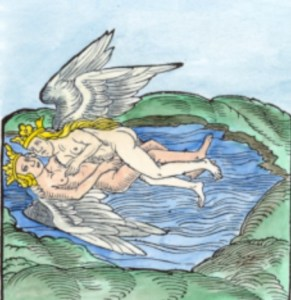
\includegraphics[scale=.4]{a20210321ReachingyourfullPotential-img001.jpg} 
\end{wrapfigure}

The first stage in esoteric teaching, the “Lesser Mysteries”, comprises everything related to the development of the possibilities of the human state. These possibilities transcend the activities of our ordinary life. The roles we play, such as family, occupation, and so on, are the fields of activity in which further development is made possible. Developing whatever talents we might have through education — the arts, science, sports, watching TV, and so on— may constitute the field of action that prepares us for higher possibilities, some obviously, better than others.

A fortiori, the search for powers or secret knowledge is fruitless, if not disadvantageous, from the esoteric perspective. These include:

\begin{itemize}
\item Fascination with vast conspiracy theories 
\item The search for psychic powers of all types 
\item The desire for mystical experiences 
\item Obsession with manifesting material objects 
\item Channeling higher beings 
\item Seeking secret knowledge of some sort 
\item Relying on psychedelics for spiritual experiences 
\end{itemize}
The common element is the focus on the corporeal and/or psychic worlds rather than the strictly spiritual part of oneself. \textbf{Rene Guenon} provides this admonition:

\begin{quotex}
[Psychic powers] are in fact a distraction in the rigorously etymological sense of the word. The one who lets himself be absorbed by the many activities of the corporeal world will never center his consciousness on higher realities, nor consequently develop within himself the corresponding possibilities. This will be all the more true for one who goes astray and disperses himself in the incomparably more vast and varied multiplicity of the psychic world, with its indefinite modalities. \flright{The “Rejection of Powers”, \emph{Perspectives on Initiation}}

\end{quotex}
This is not to deny the possibilities of such manifestations, which may arise as side-effects of mystical evolution. Nevertheless, our higher possibilities are not tied to any specific talents or abilities, since they are the principles which make those actions possible. From higher to lower, these are:

\begin{itemize}
\item True Will 
\item Consciousness 
\item Real I 
\end{itemize}
The attainment of these faculties completes the evolution of the possibilities of the human state, lifting the being to the Primordial State. Boris Mouravieff summarizes this succinctly:

\begin{quotex}
It is by this evolution that animal man can overcome Adam's Fall, can become a spiritual man, and so be initiated into divine wisdom. 

\end{quotex}
Then he is prepared for the Greater Mysteries.

\paragraph{Obstacles}
\begin{quotex}
Many are called but few are chosen. \flright{\textsc{Matthew 22:14}}

\end{quotex}
Here we encounter some immediate obstacles that prevent or discourage seekers.

\subparagraph{Unnecessary}
People believe that already have those faculties of a True Will, Consciousness, and a Real I. Hence, they don't see the need for esoteric training. They become more interested in phenomena.

\subparagraph{Explicit knowledge}
This type fails to understand the distinction between explicit and tacit knowledge. Explicit knowledge can be communicated through the written or spoken word. Tacit knowledge, on the other hand, cannot be communicated in that way. It is more like “knowing how” rather than in knowing. Tacit knowledge comes only by doing.

Like riding a bike or learning to swim, one has to actually do it. Reading a book about biking or swimming won't do it for you. Tacti knowledge is more effective if there is a guide, but most people are satisfied by reading or hearing theories about biking or swimming.

\subparagraph{Hard work}
\begin{quotex}
We can buy food for others; we can cook a dish with this food; we can serve it once it is cooked; we can cut it up; we can even act as if to put the food inside the mouth, as we do for a child or sick person. But at this point, each of us must make the necessary effort to swallow the food for ourselves; this cannot be done by anyone else. \flright{\emph{Gnosis I}}

\end{quotex}
Few people have the stamina or discipline to perform the exercises that transform explicit knowledge to tacit knowledge.

\subsubsection{Self-knowledge}
\begin{quotex}
When we close our eyes in an attempt to meditate, we are amazed to discover a boiler factory inside of us. \flright{\textsc{Joel Goldsmith}, \emph{The Art of Meditation}}

\end{quotex}
Meditation is sold today as an absolute good, that will relax us, lower blood pressure, and so on. However, if done properly, many, who believe that their inner life is nothing but Sunshine and Lollipops, are shocked to witness the “boiler factory” of irrelevant, fearful, or anxious thoughts that cast doubt rather than certainty.

It takes effort and persistence to get past that point.

\subparagraph{Inequality}
This teaching is the hardest to accept:

\begin{quotex}
Among several persons who receive an identical teaching, each one understands and assimilates it more or less completely and profoundly according to the range of his own intellectual possibilities, and in this way selection, without which there could be no genuine hierarchy, comes about quite naturally. \flright{\textsc{Rene Guenon}, \emph{Man and his Becoming according to the Vedanta}}

\end{quotex}
\paragraph{Higher Centers}
As mentioned in \textit{The Descent of the Absolute}\footnote{\url{https://www.gornahoor.net/?p=14019}}, the Emotional Center (animal soul) and Intellectual Center (intellectual soul) are divided into lower and higher centers. As we are born, the higher centers are undeveloped and are therefore only virtual. Esoteric training starts with the proper awakening or development of the higher centers.

Since our untrained emotional life is so erratic, mastery over the expression of the emotions is imperative in order to make further progress.

The Higher Emotional Center is located in the Heart, the seat of our Real I, the Sun center of our being. The Higher Intellectual Center is located at the level of the Head, the seat of consciousness.

\paragraph{Objective Art}
The first step in the in the development of the higher emotional center is to mitigate the effects of negative emotions. That opens up some space for more subtle emotions to manifest. Aids in the process include objective art, myths, and symbols. The focus of personal art is on the personality of the artist, while objective art is the reflection of higher ideas. The following passage refers to why, according to Plotinus, a sculpture is more beautiful than the block of stone from which it was carved.

\begin{quotex}
The real question is, why is the sculpted stone more beautiful? “The matter did not have this form, but it was in the one who thought, and before it came to the stone; but it was in the craftsman, not insofar as he had eyes or hands, but in that he shared in art” (Enneads V.8.1.16–19). If the sculpted stone is more beautiful than the lump, this is because thought, or idea, is more evident in it. The distinctive beauty of the sculpture, as opposed to the lump, is the form that it has received through the artist's work, which is an image of the form existing as pure thought-content, or idea, in the artist's mind. Consequently, the form, that is, the beauty, that renders the sculpture pleasing to behold is first and more truly in the artist's mind, as the paradigm of which the sculpture's beauty is an image. \flright{\textsc{Eric Perl}, \emph{Thinking Being}}

\end{quotex}
\paragraph{Myths and Symbols}
The purpose of Myths and Symbols is to reach these higher centers, the higher emotional and higher intellectual centers respectively. The attempt to understand myths and symbols by the lower mind will result in misinterpretation.

\paragraph{Sexual Sublimation}
Sexual energy can be redirected to the higher centers, which is the means to produce results.

\begin{quotex}
This consecration is produced by the sublimation of sex. Thus the circle closes itself. Each manifestation of life starts by a sexual act; at the end of the cycle, the activity of the sexual centre is manifested once more, but on a higher level, that of the higher centres, the level to which — by its nature — this centre belongs. \flright{\textit{Gnosis I}}

\end{quotex}
Ultimately, individual and group work will be replaced with Hieros gamos or polar couples. Since each one of the pair has a different way of knowing, their shared experiences enhance each other.

\begin{quotex}
The means … is to work as a couple. We must believe that in the new era which approaches, this method will be favoured more and more, will be protected, and will eventually become obligatory. However, for this esoteric work to be completed successfully by two people, it is essential that the two beings — man and woman — are integrally polar. 
\end{quotex}
\flrightit{Posted on 2021-03-21 by Cologero }

\begin{center}* * *\end{center}

\begin{footnotesize}\begin{sffamily}



\texttt{Greg on 2021-03-22 at 10:59 said: }

As to exercises does the form of Meditation matter? Is the Jesus prayer or say centering prayer effective in attaining these states or are other forms of exercises needed?


\hfill

\texttt{Tannheuser on 2021-03-22 at 12:47 said: }

I was actually just discussing this question of Objective vs. Personal art last night. 

I used the term “arbitrary” to describe what you call Personal art – to me it is boring because it does not participate in any universal idea or higher reality. That kind of art is usually a waste of time, because it doesn't offer any valuable possibilities to the one participating in it – just “A influences” imposing themselves and insisting on their own importance.

Interestingly, in contemporary art and entertainment, this arbitrary personal quality is the strongest in the so-called “high” arts (modern opera, painting, orchestral music, sculpture, architecture, and so on). Low or popular art often expresses less personal, more universal ideas, in the same way that folklore can preserve an echo the original spirit of a civilization long after the high art has become degenerate. Recently, however, there is a concerted effort to replace everything traditional even in low art with political propaganda (extending as far as 60 year old children's picture-books).


\hfill

\texttt{Arthur Konrad on 2021-03-23 at 09:20 said: }

@ Tannheuser,

Ever since the 19th century, opera and orchestral music is mostly an elaborate cacophony, operating on the same principle as a kid's toy made to produce some fabulous sound, after which the kid in question mutters `oooohhhh!' in awe – in other words, it is infantile. This is why Nietzsche loved Wagner, he had an infantile mentality. Most 19th century music was tailored to the tastes of women and effeminate men. Some operas of the romantic era are downright embarrassing. The bottom one and a half octave on the piano serves pretty much the same function. Most `virtuoso' pianists today play in a cacophonous way and abuse the bottom octaves as a rhythm section, and they think that a correct tempo does not exist. If you have healthy ears, you might as well shun piano performances for good, that thing is never going to get better.

Compare that nonsense to the masterpieces that are Baroque operas.


\hfill

\texttt{Paulo Adolpho on 2021-03-24 at 22:50 said: }

“A fortiori, the search for powers or secret knowledge is fruitless, if not disadvantageous, from the esoteric perspective. These include:

Fascination with vast conspiracy theories”

Cologero, why studying conspiracy theory, would it be negative? Don't you see that we must become aware, of who is trying to control and destroy this world, the anti-traditional forces?


\end{sffamily}\end{footnotesize}

\section[Some Observations Concerning Guenon...]{Some Observations Concerning Guenon, Initiation, and Spiritual Exercises}

\begin{quotex}
All that exists potentially is advanced to actuality by the agency of something which is actually what the other is potentially: the partially potential by that which is actual in the same partial respect, and the wholly potential by the wholly actual 

\flright{\textsc{Proclus}, \textit{Metaphysical Elements}, Proposition 77} 

\end{quotex}
Every so often one hears of conversations, or reads essays contrasting \textbf{Rene Guenon}'s views of initiation and spiritual practice against those of other initiates, such as \textbf{Julius Evola}, or \textbf{Frithjof Schuon}. In certain of these, one tends to find Guenon characterized as overly ``conservative" and ``bureaucratic", or perhaps less flatteringly, as ``cold", ``dry", and exceedingly ``logical"; his emphasis on initiatic doctrine, and regularity of a chain, appears to cause many readers of Guenon to develop an opinion that he only regarded a rigid, formal, inflexible initiation rite as necessary, and of sole importance, to the exclusion of any other possibilities, or efforts. While undeniable that Guenon stressed the regularity of chains, and meticulously sought to differentiate the doctrines of traditional initiation from ``occultist" and ``spiritist" pseudo-initiations of his own era, he did so in the hopes of preventing further decay of what did remain of a traditional character, and yet never without fundamentally maintaining that regardless of just how regular an initiation might be, it must always accompany an inner work. Mincing no words on the matter, he remarks in \textit{Perspectives on Initiation} that ``Initiatic teaching, outward and transmissible by forms, in reality is and can only be—we have said this before and stress it again—a preparation of the individual for acquiring true initiatic knowledge by personal effort (203)".

The notion that Guenon was ``too heady" and therefore ``cold" likely arises from those who would take the written word of Guenon, as tantamount to the personhood of Guenon. Indeed, he wrote with staggeringly logical precision—but was no logician, frequently explaining that though metaphysics could be presented in a logical fashion, it is superior to logic; that the representation of metaphysical teaching discursively, is not the same as realization of that teaching, although serving as an advantageous departure point, yet insisting that ``Whoever clings to reasoning and does not free himself from it at the required moment remains a prisoner of form, which is the limitation by which the individual state is defined (supra, 209)".

Others have argued that Guenon offers few solutions to the problem of degeneration and disappearance of regular and effective initiation in the West, outside of either Freemasonry, or Compagnonnage—and more so, that he quickly condemned any attempts at esoteric knowledge outside of those parameters. But again, it would seem Guenon was exercising a precise caution, while attempting to ingrain reliable ``landmarks" in those either already on, or seeking a ``path". Could it be believed for example, that Guenon, while living in Egypt, as devout Muslim and ardent Sufi would have been unfamiliar with the Sufi practices of certain orders, who perform rituals and vigils at tombs of prophets and saints, in effort to invoke barrakah, and participate in a silsilah-chain with deceased masters, and moreover, that such rituals often entailed an ``istikhara", that is, ``dream incubation"? This would all seem unlikely, but his reluctance to discuss such things was probably due to reservations that such doctrines would quickly, especially in his era, be misunderstood and rapidly associated with ``spiritism"—which they are not. Still, in his chapter from ``Perspectives", on ``Initiatic Centers" these sort of practices are alluded to when Guenon is speaking of a ``double hierarchy" within initiatic orders, particularly when an order has reached a phase of becoming externalized to a greater extent, what stands above and behind the physical leadership (who may have forgotten their true roles), is the presence of ``invisible" and ``unknown superiors". While perhaps unbelievable to some students of Guenon, he elaborates:

\begin{quotex}
All this permits us to glimpse among the many possibilities of spiritual centers certain means of acting which are quite different from those ordinarily attributed to them, and which are especially evident in abnormal circumstances…that do not permit…apparent regularity…a spiritual center of any kind may thus also act outside its normal sphere of influence, whether in favor of individuals particularly qualified but isolated in a milieu where the darkness has reached a point that almost nothing of tradition remains and initiation is precluded, or…as reforging an initiatic chain that has been accidentally broken…it is essential to remember that even if an apparently isolated individual succeeds in gaining a real initiation, this initiation is spontaneous in appearance only and will always involve some kind of attachment to an effective center (supra, 65). 

\end{quotex}
For an individual having received a regular initiation (virtual or effective), or such a ``spontaneous" initiation as described above, Guenon indicates that there are means of support for the being's continued progress, even if an order has essentially lost or forgotten its ``operative" methods. In ``Initiation and Spiritual Realization", Guenon in a brief chapter turns our attention to the doctrine of ``upaguru", an influence that triggers or elicits a spiritual or initiatic process, remarking that this function might manifest as another person, or present itself as a situation, circumstance, or even some object. When arising as a person, it matters not if the person fulfilling the role, realizes what it is they are doing because ``…in reality the true cause is found in the very nature of the one upon whom the action is exercised". The upaguru is not though, something entirely random and ``objective", as it is an ``auxiliary" and ``prolongation" of the being's actual guru—and although upaguru might manifest on numerous occasions in the being's life, each manifestation elicits something specific, after which it is no longer upaguru (104-105).

What though might be said though of the initiate who has no guru by which upaguru could be extension or prolongation? In one type of case, as in orders that operate through ``group work", the role of a human guru is replaced by the ``spiritual influences" behind the work, which of course relates to what was said above concerning the influences of ``spiritual centers". While Guenon insists that a guru (either human, as the influences behind group work, or the influences behind the rare ``spontaneous initiation") are indispensable for the initiate, such is only true so far as the ``first stages"—meaning, the conferral of an initiation to begin with, initiation as ``beginning" proper, which is to say another way, the establishment of communication with the higher states. Provided that one or more of these conditions have been met (which as noted above always also implies a continuous attachment to a spiritual center, with or without attachment to a physical center) the continued process of spiritual realization need not necessarily be dependent upon a human guru since ``…the human guru is in reality only an outer representative and `substitute'. as it were, of the inner guru…whether or not there is a human guru, the inner guru is always present, since it is one with the very `Self'. whether in order to manifest itself to those who are not yet capable of having an immediate consciousness of it, it takes as support a human being, or a `non-incarnated' spiritual influence, is in the final analysis, only a difference of modality that changes nothing essential (124)".

With all of the foregoing considered, it becomes clear that consideration of the inner work does frame Guenon's views governing initiation far more than are generally acknowledged, to summarize what this entails, he remarks ``Indeed since all knowledge is an identification, it is evident that the individual as such cannot attain to knowledge of what lies beyond the individual domain…any knowledge that can truly be called initiatic results from a communication consciously established with the higher states (207-208)". This therefore accurately describes both the dilemma of Guenon's initiation, and the solution. Knowledge is the unification of knower-knowing-the known; but, the individual ``as such", that is proceeding no further than beyond the faculties of individual mode (of which mind is the limit), as he mentions, cannot enter into knowledge of super-individual states; yet, it is by means of initiatic transmission (regular or spontaneous), the presence of a guru, or a ``spiritual influence", that must usher the ``first stages", after which, in tandem with inner work, the chasm is crossed, since it is not mind, but Intellect, the noetic faculty which enters into said communication.

Another debate that still seems to go back and forth about Guenon and possibilities of a Western initiation, involves his rejection of the Christian sacraments as initiatory—the reasons for which he précised in both ``Perspectives on Initiation", and in the article ``Christianity and Initiation"–but he said more than just that concerning the sacraments, which tends to get short shrift. Yes, he argued that once Christianity ``exteriorized" as religion, from tariqa, the sacraments (although efficacious in the religious domain), could not in any event remain efficacious initiatically; so, although remaining beneficial to the human being in individual mode (``securing" and prolonging the human state post mortem, as opposed to possible disintegration of that state), they could not of themselves any longer take the being beyond the human state. What tends to gets ignored though, is that he added to this that they could however become initiatory, if a qualified being has the ability to ``transpose" them beyond the domain of religion, in a reversal of the process leading to their exteriorization so to speak, returning them to their principle, noting ``The truth is that the sacraments cannot indeed have such effects by themselves…but…the exoteric rites can, in a certain way, be transposed into another order in the sense that they will serve as a support for the initiatic work itself and that consequently their effects will no longer be limited to the exoteric order (17)". Naturally, their use as such ``supports" is contingent upon, as in the various foregoing scenarios, that the person is, in one or more of the senses outlined earlier, already an initiate.

Regular initiation for Guenon, is then inclusive of additional varied nuances, often glossed over. In ``Studies in Masonry" he defines regular initiation, as ``orthodox", by which he means, not something ``static" or ``mainstream" (a common, modern reaction to the word), but ``correct teaching", in so much that it is correct, because it is whole, complete, originates in metaphysical unity, and points back to it. Far from suggesting something awkwardly rigid, and smacking of the ``letter of the law", employing the same argument opposed to the possibility of repetition within the Absolute (total possibility), he declares

\begin{quotex}
One can then say that it is impossible that, for two different individuals, there should be two initiations exactly alike, even from the outward and ritual point of view, and all the more so from the point of view of the inner work of the initiate…This is why we have said that initiate teaching can never take a `synthetic' form, but on the contrary must always remain open to limitless possibilities in order to preserve the prerogative of the inexpressible (Perspectives, 203-207). 

\end{quotex}
Something of a reciprocal relationship exists between Freemasonry and the Christian sacraments. Excluding for now the variable nuances and ``spontaneous" initiations, Guenon does see as one of the only regular initatic orders surviving in the West existing in Freemasonry—although its character has become virtual; at the same time, the sacraments while effective, are limited to the exoteric. The rites of Masonry lead toward the primordial and super-individual states, yet are latent or deferred; the sacraments pertain to the human individuality and ``save", but do not ``deliver". The former must be made effective; the latter need be transposed.

Hellenism has transmitted a great deal to the West in general, and not surprisingly both Masonry and Christianity have been heirs, especially of Hellenistic spirituality. In Masonry for instance, where traditionally practiced, a special emphasis is placed upon the ``Chamber of Reflection". In the Western and Eastern Churches there is the sacrament of ``Confession", ``Penance", or ``Reconciliation". Algis Uzdaviny's explains in his ``Philosophy as Rite of Rebirth" that beginning with Egypt, and flowing into Hellenistic Philosophy, especially among the Stoics, that a particular pagan practice, as part of their method for initiation, ascent, and ``returning to the primordial state", included public confessions of their ``sins" (for practical purposes, let us substitute the word ``privation" for ``sin", as ``sin" too has lost most of its meaning, signifying to contemporary minds silly sounding infractions against wanton formalism, such as eating meat on a Friday; whereas the Church had, and the Eastern Church still mostly does, regard sin on a ``sliding scale"–that is, the spiritual damage of an act, or act of omission is proportional to the way in which it limits ones spiritual progress, which is why there once were ``confessors"–elders advanced in spiritual gymnastics, and learned in life, who could assist one in assessing the impact of such matters. Ironically, while such a notion is repugnant to modern minds, they will spend fortunes on ``therapists", ``life coaches", and ``councilors" to express their ``inner demons", in exchange for nothing but more profane information, and drugs that provide no remedy!).

Quite akin to Guenon's explanation that fundamental to initiatic science is transition from individual mode, toward increasingly less restricted states, Pierre Hadot describes the purpose of spiritual exercises and Philosophy in antiquity as promoting ``The movement of the soul from individuality to Universality". Hadot explains that for our Hellenistic Philosophers, this movement from individuality to Universality is marked by three key concepts and objectives:

1. Coming to see the insignificance of human affairs, profane affairs

2. Developing a certain ``contempt" for the notion of death, or how death is understood by the profane world

3. Attaining to ``Universal vision" characteristic of ``Pure thought"

In his book ``Spiritual Exercises", Hadot examines and discusses the various types of ``askesis" or methods employed by the Hellenistic Philosophers. Drawing upon the record of Philo of Alexandria, he relates seven major askesis employed in the ascent, and then consolidates them into three essentials:

1. Prosoche

2. Dialog

3. Learning to die (Philosophy itself)

While certain of these askesis are engaged through rhetorical and dialectical teachings of persuasion, skill in rhetoric and dialectic contribute to mastering one's inner dialog and concentration, thus lending itself nicely to prosoche. Prosoche, which is ``self-attention", or ``mindfulness", is closely connected with nepsis, spiritual watchfulness, and ``Guarding the Heart" (Center)–well enough known to students of Philokalia. It is also the significance behind the Masonic ritual ``Chamber of Reflection", as well as sacramental ``Confession"—neither of which, in their deeper meanings constitute a ``one time" symbolic rite, nor an occasional ``penance" to ``meet ones obligation"—but intended as habitual activity, with increasingly greater strides in success. The choice of beginning here with sacramental confession and the chamber, in connection with inner work aimed at the ``making effective" on one hand, and ``transposing" on the other, further in relation to prosoche, is deliberate. Confession is the sacrament following baptism; while second in order, it is really only the first requiring an active participation, as baptism, even when performed on an adult, is more of an acquiescence. Confession then leads to reception of the next sacrament, which is Eucharist or Communion—union with the Body of Christ as Church, and union with the ``Real Presence" of Christ in the Eucharistic species—which is (among other levels of meaning), an Anamnesis (``Do this in memory of Me"); if ``transposed" to the metaphysical (as an aseksis) it becomes Anamnesis of the ``Real Presence" of the central ``Self", which previously we observed Guenon identifying as the ``inner guru" itself. In this way we might come to understand how a sacrament can ``become" initiatic—how, as Guenon wrote, something exoteric can be taken as a ``departure point", and ``foundation", to be ``transformed" (another observation that can be drawn from this, is as Guenon often pointed out, that there never can really be any ``contradiction" between the exoteric and esoteric orders as the lesser is always included in the higher, and proceeds from it—an important observation, as so many seeking an ``esotericism" imagine it to do with meanings that are somehow repudiations of exoteric meanings). As was also noted among Philo's list, Prosoche is the bedrock of the Philosophical exercises toward ascent.

Hadot explains that for self-attention to begin, it presupposes ``examination"; again, what is found in the sacrament under consideration, and occurring in the ``Chamber", where the candidate surrounded by images of death, left alone as if in a tomb, is instructed to consider their life, and prepare a will. And indeed, the chamber is a tomb, in which one dies to the profane world, to be ``born" in the Lodge room (emblem of Kosmos/Universality)–which Guenon refers to as ``the first death" and ``second birth" (second birth for obvious reasons that it occurs after natural birth, and death to the profane world). Per Guenon, this phase of the Initiation process entails a ``psychic regeneration", the re-collection, recollection, anamnesis of the ``intellectuality" of primordial man, by ``gathering what is sown". Still, like confession, this stage is but ``preparatory" for, as Guenon notes ``the second death and third birth" which is a ``resurrection". In a certain way then, although not exact, these relationships drawn between the use of an askesis (prosoche in this account) for the purpose of ``transposing" a sacrament, and ``actualizing" an initiatic doctrine, might analogically be expressed thus–prosoche/confession is to memory of the Real Presence as prosoche/chamber of reflection is to initiatic birth.



\flrightit{Posted on 2013-01-05 by Frater M }

\begin{center}* * *\end{center}

\begin{footnotesize}\begin{sffamily}



\texttt{David on 2013-01-06 at 00:42 said: }

This was very insightful. The last two paragraph are very interesting, but I will need to read more on the subject to understand everything. Could you tell us where next to read about this ? Thank you.


\hfill

\texttt{Pickman on 2013-01-06 at 02:48 said: }

Soundly observations my good fellow Mercurius, welcome aboard (the ship that still requires an anchor some might say). Now outside of sterile academic method, will it ever be possible to achieve a living order, not derivative of subversive Islamic or masonic currents for a re-invigoration of European man?


\hfill

\texttt{Mihai on 2013-01-06 at 12:49 said: }

You wrote quite a lot here and most of it is sound. 

I would, however, want to point out one issue I have with Guenon's view on initiation, apart from questions of ``spiritual bureaucracy", that is the particular question of the Christian rites. 

Guenon's arguments that the ``exteriorizing" of the Christian faith led to their becoming inefficacious in the esoteric domain, like Schuon rightly pointed out, do not hold water. If " what God has joined together, let not man separate"(Matthew 19:6), then there is no reason to suppose that historical contingencies can cause a God-established rite to ``withdraw" its efficacy. Rather their ``transposition" on the esoteric plane depends on the quality of the person receiving them and on the guidance (or lack of it) that certain person receives. We can say that, in Christianity, the degree of exoterism that one attaches to a rite is a reflection of the degree of his understanding (by this not meaning mental understanding). 

Reading pages from the Philokalia, one finds there ample teachings of spiritual methods and scripture interpretations that do not fall short of any esoteric ``requirements". 

One more proof: the fact that in the Hesychast tradition of the East, there is no other requirement for its practice apart from Baptism (which is truly an initiation) and the will and inner disposition of the person undergoing it, plus a truly qualified spiritual guide- this last requirement can prove quite a challenge nowadays.

I have seen that some, following some remarks made by Guenon, claim there exists a ``hesychastic initiation", that is a further rite that one has to undergo in order to practice the Prayer of the Heart. Such a claim is entirely false, as there exists no such additional rite, as the testimonies of many followers of this path attest.

Also, if Guenon admits that the Mysteries where, in their initial period, completely esoteric and than become exteriorized, then one has to ask: where did that additional rite come from ? And if it was there from the beginning, but hidden, then what was Baptism for, if it was supposed to correspond to an esoteric initiatory rite (which, by the way, the works of Dionysius the Areopagite attest) ? Why did these two rites function in parallel ? 

Finally, one cannot fail to notice that Guenon puts the Christian rites and those of Masonry to a double standard.

He rejects the claims that Masonry has become totally ineffective due to its complete degeneracy, arguing that it still holds, at least ``virtual", initiatory power, but then goes on to declare the Christian rites as ineffective because of their ``exteriorizing", even though Christianity has never fallen to the degree of degeneracy that Masonry has.

I do regard Guenon's defence of the alleged validity of modern Masonry to be the lowest point of his teachings, considering that, not only the masonic lodges fell to a level of complete spiritual ignorance, but they also played an outright subversive role that contributed to the destruction of traditional Europe. To think that one can find any trace of living spirituality in a masonic lodge today is an illusion. 

Other than these observations, Guenon's works regarding initiation are very helpful in clearing the smoke and dispelling the many delusions promoted today in ``occult bestsellers" and the like. They should be a ``must read" to anyone interested in engaging on an esoteric path, lest one falls victim to the numerous counterfeits that circulate today.

\hfill

\end{sffamily}\end{footnotesize}

\section{True Consciousness}

\begin{quotex}
He seems to be a proclaimer of foreign gods. \flright{\textsc{Acts 17:18}}

\end{quotex}
\paragraph{Natural Man}
In \textit{Ascent to the Divine}\footnote{\url{https://gornahoor.net/?p=10801}}, we described Augustine's ladder of ascent. The three lower stages describe natural man. Although the I or ego of the natural man will move among the three lower stages, each man is centred predominantly in one of the three. This centre colours his grasp of reality.

Medieval man was spiritually oriented, so he regarded thought as an opening to a reality beyond himself, either beneath him or above him. For example, concupiscence and malice were attributed to effects of the Fall, not as part of a man's very essence. That is why such impulses and fantasies were seen as originating from subhuman forces, underground, beneath the earth. So medieval man attributed the origins of such ideas to another being, the devil. Rather than being hypnotized, this was rather a truer grasp of reality. For him life was a battle, a spiritual combat, between the higher and lower forces that he experienced in consciousness.

On the other hand, as modern men have fallen deeper into materialism, the sense of thought as the revelation of something transcendent declines. While remaining oblivious to higher forces, he regards the lower impulses as his true nature. Even for the religious, spiritual combat has become pro forma, without any real commitment or understanding.

\paragraph{The Union of Opposites}
\begin{quotex}
Like a bridegroom Christ went forth from his chamber …. He came to the marriage-bed of the Cross, and there in mounting it, he consummated his marriage. And when he perceived the sighs of the creature, he lovingly gave himself up to the torment in place of his bride, and joined himself to her forever. \flright{\textsc{St. Augustine}, \emph{Sermo Suppositus 120}}

\end{quotex}
\textbf{Carl Jung} quoted that passage in \emph{Mysterium Coniunctionis} to illustrate the union of opposites. \textbf{Edward Edinger} in \emph{The Creation of Consciousness} offers an explanation:

\begin{quotex}
The coniunctio of opposites is not generally a pleasant process. More often it is felt as a crucifixion. The cross represents the union of horizontal and vertical, two contrary direction movements. To be nailed to such a conflict can be a scarcely endurable agony. \flright{\textsc{Edward Edinger}, \emph{The Creation of Consciousness}}

\end{quotex}
That explains why such inner conflict is assiduously avoided. People therefore will gravitate to one side or the other. However, Edinger explains the effects of the union of opposites.

\begin{quotex}
The union of opposites in the vessel of the ego is the essential feature of the creation of consciousness. Consciousness is the third thing that emerges out of the conflict of twoness. \flright{\textsc{Edward Edinger}}

\end{quotex}
In spiritual practice, inner conflicts are deliberately courted precisely in order to enable the ego to attain to greater consciousness.

\paragraph{Dueling Selves}
In a series of lectures delivered in 1939 in Rotterdam, \textbf{Valentin Tomberg} speculated on the inner meaning of the Crucifixion of Christ. He draws two opposing, but reconcilable, conclusions:

\begin{itemize}
\item Christ descended into Hell 
\item ``I am my Father are one" 
\end{itemize}
That is, there are both a descent and an ascent. These two movements resulted in a separation between the lower I, or ego, and the higher I, or conscience. In descending into Hell, the interior of the earth, he redeems the ego from the devil as described above. The higher I was then opened up to experience the spiritual world. This is felt initially as conscience, that is, as Christ a judge. However, the requisite purification of the mind and the will is not an easy task. As long as the lower and higher I's are disunited, the sense of conscience will be resisted. Its psychological effect is described by Edinger.

\begin{quotex}
The experience of being a known object, being seen by the Eye of God, can be a fearsome experience because unconscious contents cannot stand to be observed. \flright{\textsc{Edward Edinger}, \emph{The Creation of Consciousness}}

\end{quotex}
Just as medieval man experienced lower impulses as alien forces, modern man often experiences this higher self as alien. Hence, he may describe it as a ``Semitic" imposition or world-denying, in contrast to the lower I which is focused on the world. In that case, it would be impossible to unite the two I's.

\paragraph{Transformation in Christ}
\begin{quotex}
Man's task is to become conscious of the contents that press upward from the unconscious. Neither should he persist in his unconsciousness, nor remain identical with the unconscious elements in his being, thus evading \emph{his destiny, which is to create more and more consciousness}. \flright{\textsc{Carl Jung}, \emph{Memories, Dreams, Reflections}}

\end{quotex}
In his book, \emph{Transformation in Christ}, \textbf{Dietrich von Hildebrand} describes a spiritual path based on phenomenology; hence, it is mostly free of metaphysical arguments or sentimental devotions. For example, there is a chapter on Self-Knowledge and one on True Consciousness. In the latter, he claims:

\begin{quotex}
The inward progress in the Christian's life is linked to a process of awakening to an ever increasing degree of consciousness. Conversion itself is comparable to an emergence from a state of somnolence. In rising from self-contained worldliness towards the reality of God, in experiencing the metaphysical situation in which God has placed him and the new light in which all things and his own self are now appearing, \emph{the person attains to a new level of consciousness}.

\end{quotex}
Hildebrand warns against contemporary schools of thought which strive to reveal the hidden motives of thought. This is the technique employed by the so-called ``Masters of Suspicion" – Marx, Nietzsche, and Freud. In this task, the Medievals were more correct than those masters.

A second form of false consciousness is that of the man whose sole goal is to master a system intellectually. Hildebrand elucidates:

\begin{quotex}
He is not filled with a genuine longing for participation in being. Knowledge is not from him a road to such participation but a mere submission to the immanent logic of an unlimited process divorced from the goal of possessing the truth. Such a man cannot even truly understand the primary function of the intellect, with the participation in being which it embodies by itself. To such a man the process of acquiring knowledge has become a self-sufficient purpose.

\end{quotex}
The unconscious remain submerged in the lower I, as though in a state of nature. Hildebrand describes this state:

\begin{quotex}
The behaviour of unconscious persons is dictated by their nature. They tacitly identify themselves with whatever response their nature suggests to them. They have not yet discovered the possibility of emancipating themselves, by virtue of their free personal centre, from their nature.

\end{quotex}
As a man awakens to the higher I, the fourth stage described by Augustine, this is the result:

\begin{quotex}
A truly conscious person has so far advanced over his nature that he no longer agrees implicitly to all its suggestions. Should an impulse of malice or envy surge up in this mind, he, actuated by his free personal centre, will seclude himself from the impulse and disavow it.

\end{quotex}
Unconscious man lives from moment to moment and is thus incapable of understanding events in a larger context. On the other hand, it is different for conscious man.

\begin{quotex}
Wakefulness means to live [in the sight of God]; to interpret everything in the context of our eternal destiny, in its nexus with all our previous valid experience. Conscious man avoids being submerged beneath things or living among them in the interstices of reality; he incorporates everything int eh objectively valid order of ultimate reality. Only the Christian can be truly conscious in the full sense of the term. For he alone has a true vision of reality proper and a true conception of God and the supernatural realm from which everything derives its ultimate meaning.

\end{quotex}
In describing wakefulness, Hildebrand comes close to Tomberg in the latter's understanding of conscience.

\begin{quotex}
True consciousness implies an intimate recognition of our defects. A person who is thus conscious, who has emancipated himself from his nature and no longer agrees automatically to its suggestions, who is awakened to a sense of his free personal centre and of the essential, express, and lasting response which God demands of him, has also cast off his illusions concerning himself. His own being is illumined by the light of God and he allows that light to penetrate into all corners of his soul.

\end{quotex}
Unconscious man is discontinuous and ununified. Hildebrand describes him this way:

\begin{quotex}
Frequently we come across people who reveal entirely disparate aspects of character, of which now one and then another prevails, so that on different occasions such a man or woman may almost strike us as a different person. According to the varying elements of his environment, which their fluctuating appeal to this or that strain in his mental composition, a person of this kind may seem again and again to change his identity.

\end{quotex}
The life of the conscious man is integral and he always remains himself. The more he suffused with the light of truth, the close he comes to the Absolute I.

\begin{quotex}
We see now through a glass in a dark manner; but then face to face.

\end{quotex}


\flrightit{Posted on 2019-02-27 by Cologero }

\begin{center}* * *\end{center}

\begin{footnotesize}\begin{sffamily}



\texttt{Jack on 2019-02-28 at 23:11 said: }

``True consciousness implies an intimate recognition of our defects."

Yes. I think this can be the basis for a critique of another kind of false consciousness, which is that promoted by new age interpretations of Eastern doctrines. The whole ``we are infinite consciousness and primordially pure" idea which is seized upon by contemporary urban ``yogis" and the like is often an evasion of real consciousness of self, which necessarily includes conscience and hence a recognition of sinfulness. They want resurrection without crucifixion, or heaven without purgatory.


\hfill

\texttt{argusandphoenix (Logres/MS) on 2019-03-01 at 21:27 said: }

``Hence, he may describe it as a ``Semitic" imposition or world-denying, in contrast to the lower I which is focused on the world. In that case, it would be impossible to unite the two I's." 

From reading what I've gotten to in Plotinus, which isn't all of him by far, he discusses ``lower" things that men or beings sink into, and which they certainly have enough light to struggle against. It's not phrased the same way, but the idea is the same as hamartia, or unrighteousness. Have they gotten around to condemning Plato and Plotinus of being Semitic? I used to have the impression that Plato's theory of participation was arbitrary (one always introduces another intermediary), but if one stops thinking of the structure of reality as a ``thing" and begins to attempt experiential relation to personal and supra-personal centers, then there is no arbitrariness at all: two persons or Beings too far apart require an intermediary, and there is no inconsistency if the intermediary is apt (no need for an intermediary of the intermediary, etc., etc.). Thank you for this concise, and fitting post.


\hfill


\end{sffamily}\end{footnotesize}

\section{Esoteric Initiatic Centers}

Every so often on social media, someone naively pleas for information on finding an ``esoteric center", as if they are like McDonald's franchises just waiting for customers. Another frequent complaint is that such and such ``tradition" does not have an initiatic, esoteric center. I don't know how they know that or even what it means.

Unfortunately, none of these fellows would recognize an esoteric center even if it had a storefront on Main Street with bright neon signs. So they read everything Guenon wrote, in no particular order, hoping for a revelation, but that don't impress me none. On the other hand, if they learned Arabic, moved to Cairo, and joined Guenon's initiatic organization, I would show some respect. But Americans don't expect to go to that much trouble.

Initiatic esoteric centers are not eagerly waiting for you to show up. And if you do, they will probably make you clean the latrines for three years before teaching you anything.

\paragraph{Cults and Centers}
One can certainly find high priced cults that promise instant enlightenment. You will make many like-minded friends. They will tell you that you are full of love. They will tell you to give up attachments but not how. In the end you might notice other people's attachments, but not your own. But remember this:

A cult is easy to find, but hard to leave. An esoteric center is hard to find but easy to leave.

\paragraph{Augustine and the Fig Tree}
Augustine had explored Manichaeism and then philosophy, yet remained dissatisfied. Even the influential Neoplatonist pagan Victorinus had converted. Distraught, Augustine sat under a fig tree in a Milan garden and pleaded with God for relief. Hearing a child's voice saying, ``Take and read," Augustine picked up his Bible and read:

\begin{quotex}
Not in reveling and drunkenness, not in lust and wantonness, not in quarrels and rivalries. Rather, arm yourselves with the Lord Jesus Christ; spend no more thought on nature and nature's appetites. \flright{\textsc{Romans 13:13-14}}

\end{quotex}
Lady Continence appears to him, and he finds himself willing to live the celibate life. The Lady is the final appearance of the Anima to him. Previous appearances include his unnamed concubine, Eve, Dido, and especially his mother Monica.

\paragraph{The Buddha and the Fig Tree}
Everyone knows the story of the young prince who was shocked when he realized the true nature of life. He went on a lifelong search. Unable to find enlightenment in any of the ``initiatic esoteric centers" in India, he sat under a fig tree, vowing not to leave until he achieved enlightenment.

Like Saint Augustine, the answer suddenly came to him and he became the Buddha. Neither one needed an initiatic esoteric center. Chew on that for a while. Perhaps your own approach has been totally misguided this whole time.

\paragraph{Lama Yeshe}
There are several aspects that made Tibetan Buddhism so appealing to me at one time, namely

\begin{enumerate}
\item It is patriarchal 
\item It is hierarchal 
\item It requires a life of prayer and meditation 
\item It has a strict moral code 
\item It has a comprehensive cosmology 
\item It has an understanding of postmortem states 
\item It has a complex metaphysical system 
\item There is a path to salvation and liberation 
\end{enumerate}
Lama Yeshe was the head of the lineage into which I was initiated. I recently found out that he was reincarnated in the body of a young Spanish man, Ösel Hita Torres. Here is a video of the fellow\footnote{\textit{Taste of Buddha: One Big Love}, \url{https://www.youtube.com/watch?v=FLLaW-kKu1g}}. He seems more interested in Bob Marley than in the Buddha. I've visited Marley's house in Kingston, where the bullet holes in the walls have never been patched up. That is the price of one love. With his swaying motions and lack of a command presence, Ösel doesn't appear enlightened to me; however, it is not my place to judge, so I won't question your opinion.

I did not listen long enough to know if any of the points mentioned above came up as a question. But they seldom do. However, I usually asked about them, once in particular about the purpose of meditating on the Buddhist cosmology painted on a Thangka. The answer was that one should visualize oneself as enlightened in the presence of the devas, gods, and buddhas.

\emph{That was my own ah-ha fig tree experience}. I didn't really need the Thangka anymore. I could find all eight points in my own Tradition, visualizing myself in the cosmology of the Divine Comedy, or alchemical diagrams, so elegantly described by C. S. Lewis in \textit{The Discarded Image}. But why discard it?

All 8 points were available to me in texts that are natural to me. There are usually bad psychological reasons to choose an alien tradition over one's own. In any case, I still practiced the 8 points, although I suspect few American Buddhists do. Otherwise, they could not fail to notice how close they are to the lifestyle of the tradition they thought they left behind.

\paragraph{Isolation}
Before you commit to an ``esoteric center", consider the consequences. Your life will never be the same again. Whatever you used to enjoy will become empty experiences. Your friends won't understand you. And it is not very pleasant, as the young Prince discovered, to see life without any illusions.

And if you quit halfway, you will be worse off than if you had never begun at all.

\paragraph{Conclusion}
If you are serious about Tradition, then start acting that way. Otherwise, the next book won't make any difference. Here are some suggestions, which you can ignore or accept.

\begin{itemize}
\item Don't assume you know what you don't know 
\item The best choice is usually to follow the path of your own nation 
\item Pray and meditate, rather than read 
\item Treat your superiors with deference and respect 
\end{itemize}

\hfill

\paragraph{Appendix}
The topic of how to read Rene Guenon often comes up. Here is a suggestion.

\textbf{Foundation}: These works are simple to understand and provide a general overview. The basic issues are explained as well as the reason that a return to Tradition is both necessary and desirable.

\begin{itemize}
\item Crisis of the Modern World 
\item East West 
\item Oriental Metaphysics 
\end{itemize}
\textbf{Metaphysical Trilogy}: An understanding of metaphysics is the necessary preliminary step. Moreover, once comprehended, it brings intellectual certitude, as apodictic as any mathematical proof. However, that is only the first step. Proper training in spiritual exercises is required in order to fully understand the texts. Ultimately, book learning alone is insufficient to achieve metaphysical realization.

\begin{itemize}
\item Man and his Becoming 
\item The Symbolism of the Cross 
\item Multiple States of the Being 
\end{itemize}
The other books go deeper into specific topics and show the practical application to real world problems.



\flrightit{Posted on 2020-05-31 by Cologero }

\begin{center}* * *\end{center}

\begin{footnotesize}\begin{sffamily}



\texttt{William Zeitler on 2020-06-01 at 17:53 said: }

Another superb post! May I, however, presume to nuance your suggestion: ``Pray and meditate, rather than read" and suggest: READ SCRIPTURE! Let at least 50\% of your discretionary reading (that is, not job related) be Scripture. And pray and meditate on Scripture too! Reading ABOUT Scripture or spirituality (including this blog) doesn't count towards that 50\%! Just my \$0.02.


\hfill

\texttt{A.M. on 2020-06-02 at 10:21 said: }

A great post and a great comment from William. Although, it's easier for me to praise such well-articulated orientations than to dig into Scripture which overwhelms me with meaning and power whenever I start to read through it.


\hfill

\texttt{Sylvan Savant on 2020-06-03 at 17:26 said: }

I'm not sure if this is the right place or time to bring this topic up, but I wanted to ask you for your advice. Since this post does seem to deal with a number of subjects one of them concerning the trajectory one should take in life, I think it would be pertinent to ask which ones would be best to avoid. 

Like many young people of my generation, I feel not only horrified but also incredibly outraged at the state which the Western world is rapidly degenerating into. I do care about what happens to my country and my society, yet people like me are treated as absolute outcasts, enemies of the people, if not downright imprisoned or even called to be lynched by the purveyors of public opinion. How can one react towards the madness of accusations and lies of the most pernicious sort that surrounds us without falling victim to indignation and anger directed at those who are responsible for bringing about this state of affairs?

It's one matter to talk about Kali Yuga in the abstract as if it were an imminently approaching but not yet present event, but to see it unfold under your very nose sometimes feels like it's too much to bear. 

Do you advocate ``quietism, resigned withdrawal" or ``active, heroic life in the world"? Is there a dichotomy between the two? And even if I do follow the oft quoted advice to just limit my activity to my close circle of friends and the local neighborhood, then how can one possibly deal with the friction which arises when these circles inevitably falter under the influence of the spirit of the age, one way or another?


\hfill

\texttt{William Zeitler on 2020-06-03 at 19:31 said: }

Sylvan Savant: IMHO, I doubt that there's one answer for everyone. I personally think about ``what good can I do where I'm planted with the resources (inner and external) that I've been given?" Meditate and pray (and read Scripture) and continually do your best to follow the Spirit's prompting. Both the `heroic' and `withdrawn' Paths have their place — the question is which is YOURs. Expect your Path become clear over time — God will almost certainly need to prepare you for His purposes (although for some He makes it clear in a `blinding flash'. That may or may not be your Path). Perseverance, faithfulness and attentiveness to the Spirit's promptings as best you can for the rest of your life is the Way! I might point out that the Greek word for Way in ``I am the Way and the Truth and the Life" is hODOS, which can also be translated `Journey’ — ``I am the Journey, the Truth and the Life." He commanded us to ``Be following Me" (the verb tense makes it clear that continual following is in mind, not just a one time effort.) You know at least some of what you need to do (e.g. pray), start by being faithful about what you know for sure that you need to do. Allow God to reveal the rest in His good time as you are ready.


\hfill

\texttt{Thomas Walker on 2020-07-13 at 10:45 said: }

Just a comment on JRs post : under the influence of reading Guenon , I joined a tariqa about 40 years ago but left it after some time when I heard one of the moqaddems saying that all Christians were in hell or going there.


\hfill

\texttt{Cologero on 2020-07-21 at 07:48 said: }

JR: There is no specifically ``Guenonian doctrine"; either he is restating Traditional doctrine correctly or he is not. The ``decay of civilisation" is inevitable … you added ``irreverible". Institutions become corrupted, duh, that is obvious. As for the current leaders, Jesus predicted there would be ``wolves in sheep's clothing", so no adult should be surprised. But Catholicism, as a tradition, cannot be judged by the limitations of its ``leaders". That should be obvious to any thinking man, but it is not always the case. Many gloat over the malfeasances of the institution because of their loathing for the Traditional form of Western civ, showing a lack of intellectual integrity.

Deviation and subversion are the tactics used to destroy Tradition. You don't need to be a very astute observer to notice them in action. Just observe who and what is under attack … it's amazing how people prefer to blind themselves rather than to see. Probably because of their secret hatred for our Tradition despite their public persona. You don't want to be one of them … or do you?


\end{sffamily}\end{footnotesize}


\chapter{Purification}
\section{Psychic Distortion}

\begin{quotex}
Living in the consciousness soul, man experiences isolation, loneliness, materialism, loss of faith in the spiritual world, above all, uncertainty. The soul has to make up its mind and to act in a positive way on its own unsupported initiative. And it finds great difficulty in doing so. For it is too much in the dark to be able to see any clear reason why it should, and it no longer feels the old (instinctive) promptings of the spirit within. \flright{\textsc{Owen Barfield}, \emph{Romanticism Comes of Age}}

We are now the sons of God; and it hath not yet appeared what we shall be. We know that, when he shall appear, we shall be like to him: because we shall see him as he is. \flright{\textsc{1 John 3:2}}

\end{quotex}
\paragraph{Types of People}
Plato identified three forces in the soul: eros, thumos, and nous. These correspond to the willing, feeling, and thinking functions of the soul, each of which has its own relatively independent centre. The once-born will be centred in one of the three centres:

\begin{enumerate}
\item Centre of gravity is sensations and movement 
\item Centre of gravity is the feeling function 
\item Centre of gravity is the thinking function 
\end{enumerate}
\paragraph{The Psyche}
Psyche, for our purposes, refers to the soul life and all its functions: thinking, feeling, willing. The Real I, or Self, transcends the psyche. A result of the Fall is that one's self-identification fell from the Self to the I of the Personality, or Ego. The Ego is the conscious part of the psyche, but it accounts for just a small part of the psyche, most of which is unconscious.

Self-observation reveals that the Ego is not unified, since there are multiple, potentially hundreds of I's, each claiming to be the Ego. Some of them may work together, creating a psychological ``complex" which takes on a life of its own.

The Ego falsely believes it is one, because of

\begin{itemize}
\item the unity of the body and 
\item a common name. 
\end{itemize}
In extreme cases, like multiple personality disorder, the different complexes even take on their own names. The task is to integrate the various parts of the personality and move the centre of gravity up from the Ego to the Self. Integration means to make whole, which means to make holy. Thus, it is a spiritual task, not merely a psychological process. That is probably why \textbf{Carl Jung} could claim that most of his patients were non-religious.

\paragraph{Resistance of the Ego}
The Ego resists this process, which it regards as death. In a way it is, since the Real I then takes its rightful place, replacing the Ego. You often hear people say something like, ``I need to contact my higher Self." Of course, the Self is never an object, but always a subject. A claim like that shows the Ego's resistance to the Self. In the The Parable of the Coach, the Ego is like the coachman who refuses to take the orders of the Master in the cabin.

\paragraph{Image and Likeness}
We are born in the image of God, although the likeness has been lost or severely distorted. The image is beyond words and thoughts, so that our awareness of it is a mystical experience.

The likeness is the image as reflected in the soul or psyche. There are three stages:

\begin{itemize}
\item \textbf{Gnosis}: Gives form to the mystical experience 
\item \textbf{Magic}: Leads to action 
\item \textbf{Philosophy}: Makes the ideas communicable 
\end{itemize}
The psyche is perturbed by negative emotions, obsessive thoughts, and insistent desires. Moreover, much of it is subconscious and not readily available to the conscious mind. That is why the likeness of God gets distorted in the psyche. Hence, it is necessary to purify the psyche so that it reflects God's likeness perfectly. We will briefly examine the distortions in the feeling and willing functions here; the intellectual function will be discussed later.

\paragraph{Existence of Demons}
As was mentioned in the previous post on Demonic Possession\footnote{\url{https://gornahoor.net/?p=10454}}, the feeling and willing functions are under the influence of demons. We are not referring to any Hollywood-style depictions. Rather, the demons are known by their effects, which can be described. This is actually an important teaching. That is because it shows that our psychic functions are not intrinsically evil, but are under the heavy influence of outside forces. This was recognized in the baptismal rite prior to 1968, which used to include an exorcism. In particular:

\begin{quotex}
In the traditional Roman baptismal liturgy, we find a sequence of exorcisms that directly represent baptism's role as releasing us from the devil's possession. 

\end{quotex}
See \textit{The Significance of the Exorcisms before Baptism}\footnote{\url{https://rorate-caeli.blogspot.com/2018/11/thomas-pink-on-significance-of.html}} for more details. Unfortunately, the exorcism was subsequently removed, so anyone baptized after that year may experience more problems.

So this is hardly a novel teaching and is verified by experienced exorcists.

There is a purpose to demonic possession: to provide the friction required to become more virtuous or conscious. Although they are part of God's plan, that does not make them somehow ``good", as some false teachings assert.

I will use the terms Luciferic and Ahrimanic to refer to the demons affecting the emotional centre (astral body) and willing function (etheric body) respectively. Keep in mind \textbf{Valentin Tomberg}'s reservations about the cavalier use of those terms in certain anthro circles to account for all sorts of unrelated phenomena. Nevertheless, they are useful.

\paragraph{Disordered Emotions}
In sound functioning, the Intellect will determine what is good, just, noble, moral, rational, prudent, or loving. The Emotions and the Will then follows the intellect. This is not the case with psychic distortions. A person finds himself subject to the capriciousness of passions, particularly of negative emotions.

Work must be done on three levels:

\begin{itemize}
\item willpower, 
\item emotional life 
\item thought control 
\end{itemize}
These must be ordered, educated, and shaped. By self-observation, the contradictions in one's psychic life become visible; in particular, one must learn to resist the outward expression of negative emotions.

\paragraph{Disordered Will}
The will is a force that manifests differently in the different levels:

\begin{itemize}
\item \textbf{Mineral}: electromagnetic forces 
\item \textbf{Vegetable}: Tropism \footnote{\url{https://www.gornahoor.net/?p=8349}}
\item \textbf{Animal}: Desire 
\item \textbf{Human}: Will 
\end{itemize}
In a disordered will, a being is motivated by desires, which then distort the thinking function to justify the desire and then to determine a way to act on it. On a more primal level, one simply follows impulses such as like/dislike, attraction/aversion, and so on, quite apart from any intelligence.

The human will is still a gnomic will, that is, it depends on deliberation. This leaves the will open to doubt, viz., it becomes double-minded, hearing the second voice. This often leads to confusion and distress rather than to liberation. This is the fate of the man who is awakening to his Real I. He then finds himself alone spiritually, without traditional support. Refer to the Barfield quote on the consciousness soul in the epigraph.

The True Will, on the other hand, means that a person is acting according to his real, unfallen nature. This is the purified will, because it will only one thing. In this case, what one believed through custom, habit, conditioning, and so on, no longer suffices. Such a person chooses his beliefs because he wills them.

\paragraph{Imagery}
The demon acts on the Will through imagery. However, it cannot manufacture images, but has to rely on pre-existing images. That is why it is so important to monitor the images the one pays heed to. Our contemporary world is full of manufactured images, designed to manipulate and control people. That is why the use of TV, movies, and related media should be reduced if not eliminated.

Although some may think this topic is off-colour, I am convinced that in this day and age, specific examples are necessary. Therefore, we can provide a study of how the use of imagery works in distorting the Will.

Men and women are typically dominated by one main feature. A very common feature is Lust, since it is so tightly tied to pleasure. Take the case of Jim, for example, who is civilly divorced, although still married, morally. Having succumbed to temptation, he goes to the confessional. He starts by confessing erotic thoughts. The priest asks him if he willingly entertained them. That is because the spontaneous arising of such thoughts is not ipso facto sinful. This is completely unlike secular psychology which presumes that such thoughts are indicative of one's deepest nature. Not at all: our deeper nature is to be in the image and likeness of God, i.e., centred in our Real I or Self.

Therefore, we attribute the initial image to the Ahrimanic demon, not to some repressed desire within. The priest then asks Jim if he looks at pornography. That is because the demon cannot create the imagery, but only rearrange what is already there in one's mind. Hence, the priest is looking for the real source in external causes. Jim denies watching pornography, but explains that he has had many girlfriends, so that the memory of sexual activity with them provides ample imagery. Thus, the demon can use Jim's own life experience against him.

This is actually good news, since our faults can be forgiven. By understanding how these outer forces act on our inner psychic life, we can learn to be liberated from such forces.

\paragraph{Postmortem Purification}
This should make it clear why postmortem purification is usually necessary. Death does not by itself remove the psychic distortions, making the divine likeness impossible without further work. Then, in the Beatific Vision, one knows God as he is, in his essence, not just in his energies.



\flrightit{Posted on 2018-11-25 by Cologero }

\begin{center}* * *\end{center}

\begin{footnotesize}\begin{sffamily}



\texttt{jonh oliver on 2018-11-26 at 15:07 said: }

I have a doubt regarding the nature of the true self, according to the conception given by Tomberg, and more specifically to the distinction that he makes of it from the vedic conception. The eastern conception affirms that atman=brahman, and thus, that by knowing our true self, we know god or the absolute. Tomberg goes against this, by stating that there are other transcendental immortal selves, that are higher than our own, that of the celestial hierarchies and the holy trinity, and that knowing them constitutes a higher level of spiritual experience.

My question is about the status of all of these different immortal selves, and whether are they really distinct, or are they just like the different qualities of god, that only have an analogical difference between them, but in the end being fundamentally the same. Everything at the highest level is indistinct in god, on what tomberg would call the world of emanation, but from a logical standpoint, i can't grasp how can there be more than one transcendental immortal and fully free self in existence, so as to allow an distinction between them. Because Tomberg affirms that in knowing our true self, we are only knowing the spiritual microcosm and not the macrocosm, which implies that these beings are separated from the human individuality. If i'm not misrepresenting what he's saying in some way, could you explain how this distinction is possible.

I know that this goes off on a bit of a tangent from the post, but i still think it's somewhat related.


\hfill

\texttt{Jack on 2018-11-26 at 21:53 said: }

Thank you for this excellent post. The last line seems to reference, and contradict, the Eastern Orthodox doctrine of the distinction between the essence and energies of God; that we can know and participate in the latter, but not the former. Could you refer me to a good Catholic critique of this doctrine?


\hfill

\texttt{Xavier Galindo on 2018-11-27 at 09:34 said: }

Jack: There is a disagreement between the EO's and the RC on whether God's ``essence can be known" –more specifically between essence-energies and Augustinian-Thomistic divine simplicity. Good sources to read about this are `Ground of Union' by Williams (very irenic), Aristotle East \& West by Bradshaw (informative but polemic, blames Augustine a lot), and (Byzantine Catholic) Fr. Klappes works (available on Academia.edu). There's a part of the Summa (in the treatise on the Holy Trinity) where St. Thomas explicitly (but respectfully) says St. John Damascene was wrong about energeia, and the EO naturally don't concede this.

Truthfully there could be a whole new Council of Florence devoted to this issue alone.

John Oliver: I wonder how your question relates to the metaphysical principle that identifies knowledge with being?


\hfill

\texttt{Cologero on 2018-12-08 at 08:28 said: }

In the future, Jonh, should you post another comment, please quote Tomberg (or whomever) directly; in other words, it is not helpful to tell me what you think that Tomberg said.

First of all, the vedas make reference to a multitude of Devas or immortal selves, so your first point is unclear.

Perhaps from a logical point of view, separate selves may not make sense. For example, F H Bradley in Appearance and Reality logically reaches the Absolute, which alone is ``real". Other selves, therefore, cannot ``really" exist.

However, the Hermetic teaching is that God made a sacrifice, or withdrawal, thereby creating a void into which created things, including other selves, could reside.

Tomberg writes about two substances and one essence … ultimately only God is ``essence" or Being, and substances are part of the world of becoming. Nevertheless, when we know our True Self most deeply, we discover that we also know God. This is not a matter of logic, but rather of gnosis or direct experience.


\hfill

\texttt{Cologero on 2018-12-14 at 22:47 said: }

@Jack, there is no intent to be polemical.

The ``energies" is rendered as ``acts" in the west, since \emph{energeia} in Greek is translated as \emph{actus} in Latin. So we do know God, in ordinary circumstances, through his acts (e.g., actual grace). However, there can be no real distinction between God's essence and existence (or acts).

A critique is not a valid starting point, but rather direct knowledge or gnosis is the only guide. For starters, I would recommend \emph{Christian Gnosis} by \textbf{Wolfgang Smith}, in which he writes:

\begin{quotex}
Gnosis in the ultimate sense, if attainable in this life at all, will be the lot, here below, of exceedingly few.

The possibility of gnosis in this life (understood as knowing ``\emph{the essence of God}``) has indeed been recognized by the Church. St. Thomas Aquinas, for example, has this to say:

``As God works miracles in corporeal things, so also he does supernatural wonders above the natural order, raising the minds of some living in the flesh beyond the use of sens, even up to the vision of his own essence; as Augustine says of Moses, the teacher of the Jews, and of St. Paul, the teacher of the gentiles."

And again, referring to eh same exalted state of gnosis: ``It is not incredible that this sublime revelation is vouchsafed certain saints without their departing this life so completely as to leave nothing but a corpse for burial." 

\end{quotex}
We remind you of the epigraph:

We are now the sons of God; and it hath not yet appeared what we shall be. We know that, when he shall appear, we shall be like to him: because we shall see him as he is. \flright{\textsc{1 John 3:2}}


\hfill

\texttt{Vimana on 2019-06-05 at 12:17 said: }

``In sound functioning, the Intellect will determine what is good, just, noble, moral, rational, prudent, or loving. The Emotions and the Will then follows the intellect. This is not the case with psychic distortions. A person finds himself subject to the capriciousness of passions, particularly of negative emotions."

It seems, then, that Schopenhauer was right that the vast majority of people have a blind and impulsive Will, but he was mistaken in his promotion of complete rejection of the Will rather than aligning it with the Intellect?


\end{sffamily}\end{footnotesize}

\section{Moral Purification of the Will}

\begin{quotex}
Man's mind is rapt by God to the contemplation of the divine truth in three ways:

\begin{enumerate}
\item He contemplates it through certain imaginary pictures. 
\item He contemplates the divine truth through its intelligible effects. 
\item He contemplates it in its essence. 
\end{enumerate}

Now when man's intellect is uplifted to the sublime vision of God's essence, it is necessary that his mind's whole attention should be summoned to that purpose in such a way that he understands nothing else by phantasms, and is absorbed entirely in God. 


\flright{\textsc{Mary of Agreda}, \emph{Mystical City of God}}
\end{quotex}

Mary of Agreda has given us the three stages of Hermetic contemplation, which are related to their Yoga counterparts in the Table~\ref{tab:PurificationWill}:

\begin{table}[h]
\label{tab:PurificationWill}
\begin{tabular}{cccc}
\toprule
\textbf{Hermetism} &
\textbf{Yoga} &
\textbf{Theophan} &
\textbf{Description}\\\midrule
Concentration &
dharana &
Spoken prayer &
Visualization\\
Meditation &
dhyana &
Mental prayer &
Mental Prayer\\
Contemplation &
samadhi &
Unceasing prayer &
Prayer of the Heart\\\bottomrule
\end{tabular}
\end{table}


In his booklet, \emph{The Path of Prayer}, \textbf{St. Thephan the Recluse} provides some basic guidance on these stages. \emph{Spoken prayer} is when we pray using the prayers of others. In \emph{mental prayer} we raise our mind to God through reflection on divine things. But these are prepatory stages to \emph{unceasing prayer} which is the constant turning of mind and heart to God.

In \emph{Meditations on the Tarot}, Tomberg describes a type of meditation based on visualization which I call Hermetic Meditation\footnote{\url{https://www.gornahoor.net/?p=898}}, which culminates in a state of Deep Silence.

\begin{quotex}
Concentration without effort, which means there is nothing to suppress and where contemplation becomes as natural as breathing and the beating of the heart, is the state of consciousness — of the intellect, the imagination, the feelings, and the will — a state of perfect calm, accompanied by the complete relaxation of the nerves and muscles of the body. It is the deep silence of desires, concerns, imagination, memory, and discursive thought. We would say that the entire being has become like the surface of calm waters reflecting the immense presence of the starry sky and its inexpressible harmony. And the waters are deep, oh how deep! And the silence increases, always increasing, what SILENCE! Its growth takes place in regular waves which pass, one after the other, through your being: one wave of silence followed by another wave of deeper silence, then yet another wave of even deeper silence … Have you ever drunk the silence. If so, you know what concentration without effort it. 

\end{quotex}
Beyond the images and thoughts of the first two stages, the third stage is a direct intuition, or gnosis, of the divine essence. It involves the Will and the Heart. But Purity of Heart is to Will one thing. A divided self or impure heart cannot attain this stage. Tomberg explains:

\begin{quotex}
It is futile to attempt to be concentrated if the Will is passionate about other things. The oscillations of the mind will never be able to achieve silence unless the the Will itself infuses it with silence. Only the still Will can render the imagination and the intellect silent in concentration.

St. John of the Cross and St. Theresa d'Avila never tire of repeating that the concentration necessary for spiritual prayer is the fruit of the \textbf{moral purification of the Will}

\end{quotex}

\hfill

Originally published on 12 April 2011 in medtarot.



\flrightit{Posted on 2023-01-02 by Cologero }

\input{201311_05Purity as Metaphysical Value}
\section{Purification of the Mind}

\begin{quotex}
This is the second section from the article titled “Purity as a Metaphysical Value” by \textbf{Julius Evola}. It was published in Bilychnis, the journal of the Baptist Theological School of Rome. It is dated June, 1925, volume XXV.

Here he relies on Patanjali's yoga sutras to describe the stages in the purification of the mind. Interestingly, he describes a further stage beyond Patanjali's highest stage of Samadhi. Not surprisingly, Evola regards Patanjali's stages as negative and passive, so he describes an active and positive stage beyond that. This he relates to the “intellectual intuition” as understood in the West from Aristotle to the medieval scholastics, and then to German idealism. This stage is beyond discursive thought, and the lack of that type of knowledge accounts for most of the common misconceptions about Tradition. 

\end{quotex}
The impurity of the mind proceeds from the passive character of common perception that (not from the gnoseological point of view, but from that of empirical conditions) it is a feeling, an impulse from the outside to the inside pursuant to the coercion of the sensible object from the outside—so that the I cannot avoid perceiving or feeling what it perceives or feels depending on various times and places. Purification comprises two phases in this order: 

The first refers to the domain of the powers of the senses, to the capacity of detaching the mind from external objects, of withdrawing it onto oneself and fastening it at will. In other words, it is a matter of the maximum platonic catharsis: “To detach one's eyes and, in general, the soul, from sensible things”—taken however not in a metaphoric or moral sense, but literally: it is necessary to liberate the various perceptive faculties that the objects enchain, violate, and contaminate and to make them free of perceiving and not perceiving—and by that, in fact, unadulterated: pure. \textbf{Patanjali} indicates the stages that can realize that way through ordered discipline, of which, in any case, one can hope to progress only through exceptional inner energy:

\begin{enumerate}
\item \textit{Pratyahara} or control and mastery of the various impressions and accidental processes of associations and thought. 
\item \textit{Dharana} or concentration on a single object or sensation, excluding all the rest. 
\item \textit{Dhyana} or absorption in a not more sensible object, but produced by the mind itself. 
\item \textit{Samadhi} or elimination of the mental object itself and conjunction of the mind with its sole naked power. 
\end{enumerate}
But this negative phase does not constitute the final instance. One does not have true purity of the mind through the capacity of detachment, but rather through its power whereby the “other”, the correlation to the material object ceases to be a condition for perception, so that the “I” can, besides not perceiving, give himself, create from himself his own perception at will. It would be a matter, then, of substituting for the form of sensible and passive perception another that is active and positive, no more receiving but producing the object from one's interiority. Such is the virtue of the Aristotelian \textit{nous poietikos}, or of the “intuitive intellect” of the scholastics, Kant, and Schelling.

Only one must note than such a positive perceiving must not be \textit{another} faculty limited to the ideal order and juxtaposed to material perception, but rather its transformation and full resolution. Elsewhere [in \emph{Essays on magical idealism}], I considered the phases of such a path: here, as a simple suggestion, we can refer to so-called “supernormal knowledge”: modern psychology has ascertained that two distinct modes of perception are possible and real, having in equal measure the character of objectivity.

One is the normal connection to the physical organs, which—from the physiological, not the gnoseological, point of view—can be called centripetal, proceeding from the outside to the inside, starting from physical impressions transmitted from the afferent system to the central brain. The second way is, instead, independent of the physical organs and has an opposite direction: the point of departure is not the peripheral physical stimulus but rather an interior apperception, which then goes on to result in terms of physical perception and also in images, according to a centrifugal course analogous to that of hallucinatory processes.

Now while the first knowledge is limited by spatial-temporal and physiological conditions, the second is in a large measure freed from them and, what would result from the latest research, tends to participate in the nature of an omniscient principle. One could therefore connect to that the meaning of perfection, of the teleion, of the “purification of the mind”. From the philosophical point of view, it would then be a knowing that would originate no longer from a particular sense object to be subsumed to a discursive concept, but instead \textit{from everything}, in order to give the particular thing its place in this—just as a limb has a place in the organic unity of the body.



\flrightit{Posted on 2013-11-05 by Aeneas }

\begin{center}* * *\end{center}

\begin{footnotesize}\begin{sffamily}



\texttt{scardanelli on 2013-11-06 at 11:42 said: }

I have been thinking about this concept of widsom being “centrifugal” and “centripedal” when considering Tomberg's second letter. It seems that there is no reason why knowledge gained from the senses, from discursive thought should have to remain “limited by spatial-temporal and physiological conditions.” This thought can be a starting point for meditation, wherein one deepens the thought. So meditation can, in a manner of speaking, raise up what is below and bring down what is above by giving form to experience of the Spirit. Wisdom spiritualizes the material and materializes the spiritual. This is only possible once one has undergone the negative phase as described by Evola.


\hfill


\end{sffamily}\end{footnotesize}

\section{Purification of the Will}

\begin{quotex}
This is a section from an article titled “Purity as a Metaphysical Value” published in Bilychnis, the journal of the Baptist Theological School of Rome. It is dated June, 1925, volume XXV. \textbf{Julius Evola} was around 27 years old at the time, which is about the median age of Gornahoor visitors. The section that preceded it is called “Purification of the Mind” and the following sections deal with the purification of the word, sex, and breath.

There are some interesting points here. First of all, there is the admission that he underwent psychoanalysis; this should not be surprising given that there were two psychoanalysts who participated in the UR group. The other is his rather odd experience of the purification of the will, wherein he felt he could not move. Has anyone else felt that? Obviously, he means something different from mere indecision, or does he?


Perhaps he did not make himself clear, but his pairs of opposites do not seem to derive from Plotinus, since the primal will is for the Good. True, the One transcends all opposites. Nevertheless, if one is not motivated by pleasure or desire, one must transcend them, i.e., become “superior” to them. The important point is that Evola is here advocating a rather austere ethic: choose the necessary over the pleasurable, the difficult over the easy, i.e., choose the path of greatest resistance. A man needs to become master of his domain, self-motivated and self-ruled. But what self? 

\end{quotex}
The impurity of the will consists in heteronomy, i.e., in its being determined by something other than itself. In western culture, because of the prevailing extroversion, the conviction that every action must have a sufficient reason is widespread, or that there must be a reason or a cause for its happening or not happening, for its happening in one way and not otherwise, and this has joined with thinking that things do not happen in a different way through a divine act. It is precisely such a mode of action that is called impure. In fact, in it, action draws its own impulse not from itself, but from a motive, reason, impulse, or object by way of appetite or aversion, etc. The will to the thing desired does not want only and nakedly itself, but something else, so that it is properly said that it is willed by that other. That is the \textit{sakama karma} of the Orientals: action based on desire, action that is not through itself, but through what proceeds from it. Purification in this case is instead connected to the conviction that \textit{the sufficient reason of an affirmation can be the affirmation itself}, rather than to the concept of an act that is done only from a pure creative impulse. One can also find the best expression of this in a passage from Eckhart:

\begin{quotex}
From this deeper principle you must do your works, without a why. I affirm it decisively: even if you do your works for the kingdom of heaven, for God, or your sanctity, although motivated by the other, even then you will not really be in the right. If you ask a true man, a man who acts from his depth: “Why do you do all your works?” he will answer you rightly only if he says: “I act only for the action itself.” 

\end{quotex}
Here it is rather important to note that the need for purification assigns both the pure and the impure, the good and the bad, in a word: not particular terms but the combination of pairs of opposites. The purity in question means full autonomy, pure possession of oneself, and in respect to that, the link to the good, the sacred, etc., is no better than any other link: if that which is called good or pure by men binds the will, that is likewise to be called impure. Hence in such order, they appeal to expressions like cleansing oneself, baring oneself. \textit{Afele panta} [from \textbf{Plotinus}, “forsake everything”]: it is necessary to cleanse oneself of everything — the “high” as the “low”, the “spiritual” as the “material” — it is necessary to reduce the will to its naked essence resting only on itself. Once that point is reached, \textit{everything} becomes equally pure, just as prior to that \textit{everything} is equally impure. And that in such an order the pure must not be said of things in themselves, but of a way to live them, the measure of which is autonomy and autarchy, so that in being compelled to call something impure, only the proof of its own impurity is conveyed.

Here a particularly subtle discipline is necessary for the fulfillment of the requirement. In fact, how to guarantee that what one wills proceeds truly from the unconditioned and not from an obscure, incomprehensible complex of inclinations and impressions rooted in the subconscious? The answer is an in-depth self-analysis, to make everything progressively emerge into the light of consciousness that previously had been taken away. Even among us today we begin to work in this direction with psychoanalysis. Beyond that, there are methods of control based on the principle, that depending on whether action is conformed or not to a hidden inclination, it will produce pleasure or aversion. Along these lines, it is not enough to believe that the alternative is indifferent, or to put aside one's own will and to leave decisions to chance; for example, by the flip of a coin. In the sentiment that results from it and extending this discipline to a topic that always more closely concerns us, we will have a real means of indicating the progress or decline along the path of the purification of the will.

In general: it is necessary to renounce everything once one feels that it becomes necessary, or once one uncovers a desire or satisfaction for it; \textit{it is necessary to do, on principle, not as one pleases, but what is required, to always take, on principle, the line of greatest resistance and, thereby, to make the will ever stronger and purer, to make self-possession ever more energizing}. Hard discipline, which one would hardly know how to adapt to unless one succeeds in feeling in the naked will, in autarchy, a stronger motive and a more intense and vaster pleasure than what things in themselves can ever offer us.

In any case, it leads to a rather difficult point, whose reflection is precisely the difficulty that common knowledge meets in conceiving an action where there is no longer a “because” to arouse it. One feels as if the entire inner being were crystallized, so that no movement is any longer possible: it is like a paralysis, an absolute aphasia, that contrasts painfully with the sense of inner possibility. Almost as if one had something to say but the mouth remains mute and inert to command.

The experience of such an inner state provides the sign of purification and for that reason the individual knows how little what he called his action was truly his, how much a real impulse was absent from his ordinary life, “higher” or “lower”, and he being not the author, but a puppet, a medium blown about by alien forces. He knows however the I, and beyond that, how to find an excess of strength, he knows in spite of all acting, that he has achieved in himself the principle of a higher life, a power that stands beyond his being made from dependency, contingency, and finitude. And the door for that higher accomplishment, which is connected to the remaining purifications, is disclosed to him.



\flrightit{Posted on 2013-11-03 by Aeneas }

\begin{center}* * *\end{center}

\begin{footnotesize}\begin{sffamily}



\texttt{n0e on 2013-11-04 at 08:22 said: }

Psychoanalysis in Evola is, i suppose, just a modern way of achieving alchemical result, uniting Sun and Moon, conciousness and unconciousness. Which would be a necessary precondition for developing maximum control by the Will of the Self.


\hfill

\texttt{JA on 2013-11-04 at 08:57 said: }

This is very similar to Crowley's teachings in Liber Aleph. I've always seen C and E as quite similar personae, I think if E had not made the fortunate encounter with Guenon's writings Baron Evola would have wound up as the Italian version of AC. 

For clarity, let's point out that this written before the Baron discovered Guenon, at the time he was still working within a modernist framework of spirituality; as he described himself in The Path of Cinnabar, hence the positive discussion of psychoanalysis which he would later condemn after becoming a Traditionalist.


\hfill

\texttt{scardanelli on 2013-11-04 at 10:16 said: }

In light of the content of the post, there seems to be a tendency amongst traditionalists to create another pair of opposites, Tradition:Modernity. There was a comment previously about Jung not being “Traditional” or in this context, psychoanalysis not being “traditional,” as if there were a list of authors one is authorized to read when one becomes a “traditionalist.” 

But it seems less a case of something being traditional or modern and more a case of “everything in its place.” If one seeks to see the self and the world through the lens of psychoanalysis (or Freudianism, Marxism, Feminism, etc) this is obviously an error, but when seen as integrated in a hierarchical fashion, as a possible tool to analyze the “inclinations and impressions” of the soul, it is neither modern nor traditional, but either a more or less effective tool. This, I believe, is what Tomberg refers to as the spirit of free research. Everything is “traditional” in its proper place. It is the breakdown of this hierarchy that is not traditional.

It seems that this paralysis Evola speaks of is only necessarily so from the perspective of the ego, and this contrasts with the inner freedom of the Spirit or Self. When one realizes this interior freedom, he sees the exterior as arbitrary and dualistic. To act in the name of good is to evoke the bad. To act for the sake of the Kingdom of Heaven is to evoke The World. So this paralysis is effectively a binding of the ego and elimination of arbitrary and conditioned action, in favor of unconditioned action, whose source is the Spirit or self. And the “[t]hief will be obliged to flee with his artifices of iniquity.”


\hfill

\texttt{scardanelli on 2013-11-04 at 10:28 said: }

Further, it seems that Evola is saying that we must not only recognize these opposites, but use them for the sake of purification of the will. I don't think Evola is advocating that we be manly men, and do what is difficult for its own sake, but to recognize our attachments and use their opposite to bring about detachment. We choose the difficult to detach from ease and comfort, not to create some perverse masochistic attachment to pain and difficulty.


\hfill

\texttt{Avery on 2013-11-04 at 10:38 said: }

“Jung does not simply return a Christian to Christianity, a Jew to Judaism, a pagan to his paganism, as he claimed. More importantly, by rendering the suppressed underground emotions conscious and acceptable, Jung legitimates the demonic and destructive as having rights of their own on the strength of their therapeutic potential.”

Philip Rieff, The Triumph of the Therapeutic


\hfill

\texttt{JA on 2013-11-04 at 15:49 said: }

It's for me to be the voice of humour and add, in reference to dear scardenelli's mention of masochism, that the practice's nomenclature derives from Baron Leopold von Sacher-Masoch; an Austro-Hungarian aristocrat, and that experimental and different tastes in sexuality are quite the norm among those of us of a higher breeding……………………


\hfill

\texttt{Scardanelli on 2013-11-04 at 22:04 said: }

@Avery, forgive my mental laxity, but I'm not sure what your point is. Is this an argument against Jung as “non-traditional”?

@JA, I suppose I'm lucky then to be the low born descendant of dairy farmers and coal miners.


\hfill

\texttt{Jacob on 2013-11-05 at 19:52 said: }

@Scardanelli: 

I assume you mean my comment. I agree with what you wrote. The Scholastics always said truth is one. 

However, I'd like to understand where is Jung's place. Some (most notably Charles Upton) seem to imply Jung is subvervise and that following his teachings would lead to confusion between the psyche and spirit. I always assumed Jung viewed God as changing and at least partly evil himself. This may be a complete misunderstanding and extremely incorrect, which is why I commented that if Cologero (someone more knowledgeable than I) believes there is something redeemable there I would take a second look. 

Still I don't believe reading half truth would be beneficial if I can get access to the full truth. To kind of illustrate my point: Giles Deleuze is sometimes said to have based his metaphysics on Hermeticism and early Christianity. As I investigated though it seems that the word desire was being interpreted differently than Deleuze probably meant it. Instead of making an attempt to reconcile Deleuze to Christianity it seems far better to simply bypass Deleuze altogether since I have far better resources at my fingertips. Even though he has intelligent points to make, I'd like to understand where he is wrong first in order to fully understand the issue. 

Anyway, sorry for the long post and I hope this did not sound combatitive, because it was not my intention a lot of communication is lost over the Internet though.


\hfill

\texttt{Cologero on 2013-11-05 at 21:04 said: }

Jacob, you can safely ignore Jung, there is nothing necessary in his works. In the “Answer to Job”, Jung describes God as unconscious, requiring man to make him conscious. Nevertheless, when Jung restricts himself to empirical psychology rather than metaphysics, he has some interesting things to say. This may be useful in our times since the predominant method of argument these days, even among neo-traditionalists who should know better, is to attack the motives or impugn the psychological states of one's interlocutor. The truth or falsity of a statement is barely considered.

At the least, Jung had an encyclopedic knowledge of religions, religious experiences, history, symbols, etc. Hence, I find reading his works of interest just for that reason. By the way, Jung had high regard for Evola's book on Hermetism.


\hfill

\texttt{scardanelli on 2013-11-06 at 11:56 said: }

Jacob,

I wasn't necessarily arguing for or against Jung. I apologize for not clearly expressing it, but I was trying describe a way to approach truth as a process that unfolds within, rather than something we search for in books. In this sense, Jung is either more or less helpful in this process. I think that for many of us, books serve as a starting point. But for too many they are also an ending point. So we become dogmatic about who we read, who is traditional, who is modern, and in the end we change very little. Reading is instrumental, but really becomes a distraction at a certain point, when perhaps more concrete efforts are required.


\hfill

\texttt{scardanelli on 2013-11-13 at 20:54 said: }

One can see an interesting parallel with this series on the purification of the will, word, sex, etc in St John of the Cross. In The Ascent of Mt Carmel, regarding practical advice for the active night of the senses in which one purifies oneself of the passions, he gives this advice:

1) Seek to imitate Christ in all things

2) Renounce any sensory satisfaction in things that does not strictly serve to honor God

3) Harmonize the passions by always choosing:

{}-the most difficult over the easiest

{}-the most distasteful over the most delightful

{}-the less pleasant over the most gratifying

{}-hard work over rest

{}-the unconsoling over the consoling

{}-the least rather than the most

{}-the lowest and despised over the highest and most precious

{}-to want nothing rather than something

4) seek to carry out these practices and overcome the will's repugnance for them

5) desire to act, speak, and think with contempt for oneself, and desire others to do likewise.

So we clearly see an accordance with Evola's discussion of opposites, and the way in which one can use one to eliminate attachment and dependence on the other.


\hfill


\end{sffamily}\end{footnotesize}

\section{Purification of the Word}

\begin{quotex}
In this rather interesting section, \textbf{Julius Evola} writes on the purification of the word. This is the fruit of his study of the Tantras, which he learned from the writings of \textbf{John Woodroffe}. We need to reemphasize that his goal is not to convince everyone to become Hindus, but rather to use those teachings to elucidate metaphysical principles. Hence, Evola in this series always relates those principles to the corresponding Western ideas. There are three consequences:

\begin{itemize}
\item It shows that such principles have been known as well in the West 
\item It points the way to the recovery of Tradition by deepening our understanding of those principles 
\item Even those who choose to look in a different direction, e.g., the re-paganization of the West, must nevertheless incorporate this understanding into their own worldview 
\end{itemize}

All things are created through the Word, i.e., it is the principle of all created things. In the process of creation, the original creative impulse passes through a series of stages arranged hierarchically\footnote{\url{https://www.meditationsonthetarot.com/the-cosmic-hierarchy}}. 

The concept of the mantra, although it goes into deeper detail, is akin to the Western notion of hylomorphism. The “idea”, or “word”, are non-dual, but as they manifest, we experience the effects as a duality between the idea of the thing and its particular manifestation. That is why to know the real “name” of a thing is to know it in its essence. We came across this in the discussion of Occult Phenomena in the case of Adam, who had the power to name things. 

Note, too, how the power of the mantra is related to the devata and matrikas, which in the West are better described as “angels” or angelic intelligences. They are in the “causal” state, which is beyond form. Since the discrediting of the works of \textbf{Dionysius the Aeropagite} by academics, the role of the angels in creation has been neglected and they have become merely sentimentalized. Here, we see Evola relate them to an idea or word, a teaching we have alluded to many times previously. \textbf{Valentin Tomberg} also advocated for a better understanding of the role of angels.

Finally, I don't know that the phenomena mentioned in the final paragraph can be empirically verified. 

\end{quotex}


At this point, it is necessary to refer to the Indian doctrine of the “mantra” and, first of all, to indicate the metaphysical principles it presupposes.

The Word (\textit{shabda}) — according to the \textit{mantra shastra} — is the principle of the totality of created things. In the system of reality and beings, there is the manifestation of an originary power of expression, a manifestation that is structured in various hierarchical grades. In order to understand that, we note that a duality is implicit in the Word: on the one hand there is the word properly called (\textit{vak = vox}), on the other, the meaning or the object that the word itself expresses (\textit{artha}). Now in the first, supreme power of the Word, called \textit{shabda brahman}, word and meaning are one and the same thing, the expression is pure self-revelation, absolute transparency of the eternal meaning in itself. However such a unity becomes altered at the point of expression properly called. In fact, in the concept of manifestation there is implicitly a duality, or a proceeding, a going toward the other (\textit{bhavamukha}). Thus what as \textit{shabda brahman} is a second absolute, individual simplicity, is articulated and distinguished in further powers of the Word.

The Word, in being incarnated, germinates, through its own proceeding, what was a meaning resolved by it and is made objective in an ex-istence. In this dichotomic process, the “supreme sound” (\textit{para shabda}) assumes two aspects. The first is called the “subtle or causal state” (\textit{sukshma, karana}) of the sound and corresponds to “nature naturing”, to the Logos in its properly creative function (\textit{hiranyagarbha shabda}): object or meaning and word here are distinct; in the second place it no longer has a unique, concise meaning of the whole, but a unity that is dispersed in a multiplicity. Nevertheless here the distinction and multiplicity are still included in the unity of a productive function; although distinct, object and word are still not external to each other. In this second power of “sound”, there is therefore an ensemble of cosmogonic functions, corresponding to the \textit{logoi spermatikoi} of Greek speculation and to the “letters of light” of the Kabbalah and which are precisely called “letters to the causal state” or \textit{matrikas} (goddess mothers) and connect symbolically to those of the Sanskrit alphabet. All things in the world would proceed from the “combination” of these letters, but not such as they appear in their effects to sensible perception, but rather what are in their causes: such are the “Names” of things. Now, in these functions of the Word, the aspect of the meaning corresponds to “\textit{devata}” (Vedic deities), and the aspect of the word or expressive corresponds to the “mantra”. The mantras would therefore be the Names of the \textit{devata}, or the various “bodies of power” that rule the productive process of things; and, vice versa, the devata would be the transcendental meanings that the mantras incorporate and bring to light.

Beyond this subtle state of the Word, there is a third material state (\textit{sthula}), corresponding to the audible spoken voice (\textit{vaikhari shabda}). That is, one stands at the level of worn-out manifestation, where the scission between \textit{artha} and \textit{shabda} is complete: on the one hand, there is the spoken language, on the other, material objects, whose relation to it is exterior: the “Name” or the world no longer has an objectively expressive or creative value, but only a conventional, allusive value of materiality, not of the inner meaning of the object. Besides, while the “natural name” or mantra of things is universal, the name which appears at this level is particular and contingent, it depends on time, place, individualization, race, etc. But beyond the various languages of men there would be, or would have been, (according to some initiatic traditions, in the period prior to the “confusion of tongues” alluded to in the Biblical story of the Tower of Babel) a type of universal language, in which each thing and each being would have its natural, original or essential Name (\textit{bija mantra}).

The word, such as it is known by the finite being, is therefore “impure”: impure first of all because it does not have in itself, in its own power, but outside of itself, the object that it expresses, because it no longer provides the real nature of the object in a productive function, but only the simple subjective image; in the second place, through the contingency and particularity of this same image, which depends on place, time, individualization, etc. Now the requirement of the practices that reconnect themselves to the mantras is exactly toward a “purification of the word”, which is: to bring the I from that language that is the evocative faculty of simply subjective images, to that other language that is the power of evoking the things themselves, that is, to the language that produces things in their causes, being identical to the its supernatural productive process.

The mantras are the “natural approximate names” of things; by means of a living compenetration in them, the yogis seek therefore to return to, or better said, to identify themselves with, the various causative powers or \textit{devata}. That is the awakening of mantras: to awaken a mantra means to evoke, regenerate, render into act, the subtle function of the Word connected to it. It is a matter of a true putting in relationship, of a real identification. The I of the order in which the word is simple evocative discourse of vague images passes on to that in which it is a creative spiritual power, however, from the plane in which the perceiving is a passion to the plane in which it is a putting (whence the connection to the “purification of the mind”). The mantra is therefore nothing if it is not “reawakened”: one can repeat it a million times—it is said in the texts—but as long as it is not known, it remains a mere flapping of the lips. The mantra must be actualized, “made to bloom” (\textit{sphota}) in its essence “made of light” (\textit{jyotirmayi}): only then does it “work”. Its pronouncement is therefore an inner act, whose material expression acts only as the vehicle. The \textit{sphota} can happen only by means of the force of will: but more often the vital force (\textit{prana}) or the force of generation (\textit{kundalini}) is undertaken as auxiliary.

Now when one realizes a state of identity with the individuating principles of things with the mantra, it is evident that, by vibrating the same will in a “reawakened” mantra, the related act has magical value (that which corresponds to it is directly realized) since what one wills is as if the thing itself wills it. So the virtue attributed by the texts to the mantra—to the “pure word”—is astonishing. Having reawakened the mantras of various elements, the yogis acquired power over them, he can, for example, make fire flare up where he wants or to go into the middle of it without being affected by it; through mantras, he can produce the well-known phenomenon of the growth of a seed into a plant in a few minutes; he can place around himself a circle that nothing can pass through: a lance or a projectile hurled against him rebounds instead against the one who threw it; he can conceal himself from the view of others, in order to provoke visions, thoughts, and feelings in them; he can kill or cure at will. In the \textit{Vishnu Purana}, the power of procreation by means of the mantra is even considered.



\flrightit{Posted on 2013-11-10 by Aeneas }

\begin{center}* * *\end{center}

\begin{footnotesize}\begin{sffamily}




\end{sffamily}\end{footnotesize}

\section{Purification of the Sex Act}

\begin{quotex}
In this section, Evola offers his comments on the purification of the generative act. Drawing primarily on the tantric writings and German idealism (especially \textbf{Fichte} and \textbf{Schelling}), but also \textbf{Clement of Alexandria} and \textbf{Plotinus}, Evola equates the woman with nature. And nature is that which is still dark or impervious to the spirit. The goal, as he sees it, is not detachment from the body, but rather its transformation into spirit, the “resurrection body”. The desire to eternal life lies in the depths of man. 

\end{quotex}
Since an act is impure or imperfect if it does not attain actuality from itself, it is evident that the generative act is like that, and in a typical way—\textit{and it can be said that the woman in a transcendental way is nothing but the symbol of the impotence of the I to give itself a body from itself}. Now, in order to understand what meaning purification has in this case, it is necessary to keep in mind what was said in principle, and that is that the imperfect act only apparently resolves the insufficiency of the agent, in reality it reaffirms it: whoever drinks, whoever asks for water that is “another” and not the eternal water that is “pure act”, and who, with Christ whom we referred to, will never have his thirst satisfied for all eternity. It follows from this that as long as the “I” asks the woman for the conditions for a generative act, he will remain in the state of privation and impurity: and the dyad and the “other” that he presupposes as such (in the duality of the sexes) can with justice only be reaffirmed in the result, i.e., it will make it so that the act is worthless as self-generation, but rather as \textit{heterogeneration} (generation of the son), whence the destiny of death.

What gives life to the son, \textit{kills} the father, which makes the “Only One” mortal, an individual [See Clement, Stromata, Book III, Chapter 9, para 63]. The act escapes from the agent and makes his life pass away. To explain it more clearly: in the depth of the individual there is an originary power that \textit{wants} life beyond temporal limits; this power, at the level of normal and \textit{extroverted} human existence, is the desire “to look outside” (\textit{bhavamukha}).

It strikes on “another” (the woman) and so the impulse for continuity degenerates, the act that should have been the affirmation of oneself (autogeneration) becomes the affirmation of the other — of the son. The resulting continuity is not then that of the individual but \textit{that of the species} — and man is drawn into the wheel of finite and discontinuous existence, dominated by the law of generation and corruption — mortal, eternally thirsty, and eternally disappointed.

This impurity of the generative act is connected to that which inheres in the very existence of a physical body. In the normal man, the conscious power falls to a great degree outside that deep principle that rules the various processes of his organism. For this reason, he does not know how to give himself a body from himself; for this reason, he is impotent against the law of corruption. As Leibniz expressed it, the “flesh”, corporeity, represents simply the indistinct and unconscious \textit{quantum} (or better: passion and privation) that is in the I, and only in this sense is it to be understood as an imperfection. And one could say that such a region of privation in the I is the transcendental foundation of the woman, since we indicated that the correlative of the generative act as imperfect is conveyed precisely in the woman.

This is, to use alchemical symbolism, the “salt” that encompasses the active and central principle of “fire” or of “sulfur” and which “mercury” must release until reconciling this same sulfur only with itself, in the flame of the divine (\textit{theion} = sulfur = divine), of that which is pure possession or perfect act and whose eternal life, whose eternal autogenesis, is precisely symbolized by the Phoenix pulling himself out of the fire.

This is the “Great Work” that has, as its direction, the construction of a “body made of freedom”, of a body spiritually transparent to itself. We are led to the doctrine of the “immortal or cosmic body”, traces of which are found in almost all the religions and is therefore based on the following premise: corporeity is only whatever is passive in the spirit, the not yet expressed, the virtual, “in potential”; it does not constitute a distinct principle, but instead is a state of privation (\textit{sterema}), a shadow in the unique reality of the spirit.

Thus it is clear that liberation cannot consist in detachment from the body, but in its \textit{resolution}. Here purification means precisely the realization, as a function of potency in act, that the material body is experienced as a function of passion — and as such, the construction of the immortal body or “resurrection body”, “body made of spirit”, “apparent body” (\textit{mayavirupa}: recall that \textit{maya} in the tantric and mahayana schools means both appearance and magical power) or body “of flames” [according to Plotinus, the body of flame is sufficient in itself and does not require food], it is the dissolution without residue of the material body in pure activity, in \textit{shuddha-sattva-guna} — it is the individual in which the negative aspect of \textit{rajas} and \textit{tamas} has entirely vanished.

It is called immortal because, depending entirely on the I, the I can make it appear or disappear, maintaining it or destroying it when he wants, for the time that he wants, in a way that the law of life and death is vanquished. It is called the “cosmic body” for this reason, it is admitted that the metaphysical principles or “divinity” that rule nature are present in the body, although only under a darkened form as if sleeping, a form which the I experiences precisely as nature, i.e., as the “other”, and not in itself as spirit. But at the point in which corporeality is entirely conquered in conscious actuality, this form, however, is less identified in the various principles of the cosmic hierarchy, and the individual goes on to feel that his true body is the universe.

Now if the impurity of the generative act is the cause of finite and mortal existence; and if, on the other hand, this existence is defined in the differential of obscurity and privation that the body as such represents; one understands how at the construction of that supreme purity that is the “immortal body” — through which the very “other” of exterior nature is dissolved — a conversion of the force of generation is associated. This is not the place to expound on the technique of such a process.



\flrightit{Posted on 2013-11-13 by Aeneas }

\begin{center}* * *\end{center}

\begin{footnotesize}\begin{sffamily}



\texttt{X on 2013-11-13 at 04:30 said: }

Sometimes Evola is deadly accurate and sharp.


\hfill

\texttt{JA on 2013-11-13 at 09:45 said: }

it's like he's trying to transcend corporal sex instead of seeing sex as the transcendent as Crowley did.


\hfill

\texttt{Jacob on 2013-11-13 at 22:08 said: }

It's great reading the same thing in different language. I feel like I understand slightly better what Serrano was getting at the whole time in El/Ella. 

I'll have to think on this some more.


\hfill


\hfill

\texttt{n0e on 2013-11-16 at 04:58 said: }

in modern terms one could say that Evola shows here metaphysical underpinnings of astral projection


\hfill

\texttt{Cologero on 2013-11-17 at 19:27 said: }

Jacob, there is an Italian saying “tradurre è tradire” (translation is betrayal). So, of course, there is a certain amount of “interpretation” along with a translation. That is, there is no univocal correspondence between a word in one language and another, so the meaning has to be grasped in order to choose the correct word or phrase. In a sense, Evola is doing something similar when he points out that a concept in one tradition is expressed in a different way in another, although the meanings are the same.

It is certainly worth the effort, as much for me as for the readers here, and it is part and parcel of learning how to read, I mean to truly read. Now a parrot has no understanding, so there is no point in just quoting long passages from Guenon, Evola, Nietzsche, etc. That is something that will get you a lot of “likes” on facebook, but no respect in this quarter.

I presume you are reading El/Ella in Spanish? Now that my health has been cleared for the time being — I've seen every specialist but a psychiatrist — I am thinking of reviving the El/Ella discussion list. I just need to decide on the best format to keep it on track. Gornahoor's time is running short and the more important work will be done in discussion lists.


\hfill

\texttt{Jacob on 2013-11-19 at 11:23 said: }

No, I was just using language in its figurative sense. I had only read some of it in English thanks to our discussion. 

But Evola expresses it at least to my mind more clearly, or maybe they were both equally clear and being able to connect that the two are nearly one and the same allows greater understanding. 

I'm really glad you're going to restart the discussion. I often feel like I'm trying to learn to paint beautifully without even seeing the colors and just hearing the sound of the brush. It's pretty much as you said grasping the concept intellectually vs. actualizing it.


\hfill

\texttt{Scardanelli on 2013-11-19 at 21:54 said: }

@jacob

I know what you mean about theoretical knowledge vs. experience. There is knowing and there is knowing so to speak.

There are a wealth of books to read but very few who can direct you regarding practical experience. I think the discussion list format is the best next step. I'm looking forward to it.


\hfill

\texttt{Thomas on 2013-11-21 at 12:21 said: }

Thank you for this very interesting extract from Evola. Is there somewhere that we can find ” the technique of such a process” either in Evola or elsewhere?


\hfill

\texttt{Sigurd on 2017-06-20 at 19:06 said: }

To what noe has replied with: is this the Great Work of Hermetic thought? To project the astral body? This passage from Evola seemed quite nebulous to me, being truthful, before I read the comments. The quasi-philosophical wording makes it quite difficult.


\hfill


\end{sffamily}\end{footnotesize}

\section{The Purification of the Breath}

\begin{quotex}
The way of the spirit is such that it does not exist for those who do not want to follow the path. \flright{\textsc{Julius Evola}}

This is the concluding section of Evola's essay on the metaphysics of purity. Once again, he expresses Eastern doctrines not only in Western terms, but also relates them to actual experiences rather than empty doctrines. He referred to this elsewhere as “metaphysical positivism”. This puts him at odds with those who deny the possibility of higher states, but, more importantly, against those of a new age bent who tend to obfuscate these doctrines due to their incomprehension.

Since there now seems to be an audience that can benefit from such writings, I may translate the related chapters of \emph{Essays in Magical Idealism} provided my energy holds up. 

\end{quotex}
It is sufficient to mention the \textit{kundalini} yoga of the \textit{Shakti tantra}, that will permit us moreover to say something about the “purification of the breath”. Roughly speaking, its meaning is the following: there is a force (\textit{kundalini}) in man that is the root of his individual unity and a principle superior to every polarity or duality. It is the Logos (\textit{shabda brahman}) in the body. However in the common man, this force appears only in an extroverted and impure form (impure because it is turned to the other) of the power of animal generation. It is a matter of realizing kundalini in consciousness, of grasping it, of separating it from that extroverted direction and then folding it on itself in a point of mastery and sufficiency. Then kundalini, restored to its true nature, makes itself the instrument for the reaffirmation of the I over all those principles that rule his physical, biological, and mental being and that previously fell outside his power. Now in order to achieve such a conversion it is necessary that kundalini be invested by something already pure and entire in order to communicate these characteristics to him. That may be \textit{prana}.

\textit{Prana} for the Orientals is the life force connected to the breath and, as one, transcends the material breach with which it can be said that it is in the same relationship as the soul to the body. Moreover, it is necessary to remember that in the metaphysics connected to such disciplines, the highest meaning of creation would be given by the mantra Hamsah: Ham would be the inhalation, Sah the exhalation, therefore hamsah is the simultaneity of inhalation and exhalation. Naturally, exhalation is symbolic of \textit{proodos} [progress], of the act of pure, demiurgic creativity; inhalation is the further power, through which the central principle “originated”, is reaffirmed, recognized, and mastered. \textit{Hamsah} has the meaning of an eternal, simple sudden intuition, the synthesis of being and non-being (sadasat) in which the Absolute makes use of a pure self-revelation or self-giving to itself. Now \textit{hamsah}, which is that in which all beings “live, move, and are” [Acts 17:28], is present also in man, but in an impure and divided form: in man, life (\textit{prana}) is no longer fixed and concentrated simultaneously, but rather it comes and goes with alternating inhalations and exhalations, in a fluctuation and a contingency that reflects the ultimate of the first inhalation of the newborn and the last exhalation of the dying man.

The yogi, through the appropriate discipline (\textit{pranayama}), directs himself to dissipate this impurity. The I must seize prana, pulling it out from fluctuation, keeping it fixed in its own body. With such concentrated and total power, he then proceeds to empower kundalini; then it is “awakened”, it detaches itself from the extroverted direction that craving desires and is related in itself; it no longer flows downward, but “upward” (\textit{urdhvareta}) [a yogi who has accomplished perpetual sublimation of semen]. In that animal generation (heterogeneration) yields to that of the gods or spiritual generation (autoctisi) [in the philosophy of Gentile, the act in which the spirit creates itself]. After making itself pure and individual activity, kundalini progressively empowers various subtle centers and changes the dualities in them into actual simplicity; that means: it realizes in the I a relationship of identity and mastery with those spiritual powers that, close to the state of privation and obscurity of the body, is opposed to it as physical nature. At the limit of the process there is the purification of that which was sexual coupling—i.e., pure auto-generation—and, in that way, the supreme liberation (\textit{paramukti}). It is said that for anyone who is elevated to this point neither the body, nor the “other”, nor dissolution, nor destiny of rebirth exist any more (\textit{kaivalya}); he lives in accordance with pure activity that previously he felt as obscurity and privation: the various functions are reawakened and intensified in the original and glorious nature of cosmic power. In particular, the I can generate, he can give himself from himself a body while also maintaining and changing it at will. Lord of the laws of life and death, he is satchitananda, i.e., conscious actuality (\textit{cit}) and insofar as perfect (\textit{sat}), blessed (\textit{ananda}).

\paragraph{Conclusion}
We believe that this brief essay on one of the most important initiatic doctrines is not entirely lacking interest; and we would certainly be pleased if anyone succeeds in getting from it some idea of the possibility of a consideration of similar topics, that go beyond both the limited attitude of those who, enclosed in rather restricted horizons, only know how to scorn and ridicule, as well as those who, like an octopus, love to muddy the waters and take for mystery and the “occult” what they are unable to understand, which on the contrary they only know how to deform with a great deal of prejudices.: and in this group, we can include almost the totality of those who speak of “occult science”.

There is instead a way to consider initiation, through which it presents a perfectly intelligible content valid in itself, proceeding moreover from a concept of man (\textit{en sarki peripolon theos}) [a god walking in the flesh], of his value, and his task, lofty and magnificent like few others. We will certainly not stop here on this question of the real possibility of similar paths. In any case, we should not neglect how much metapsychics today is little by little verifying as effectively possible for man. On the other hand, it remains in fact that a number of things are impossible only because we do not believe that they are such; and that \textit{the way of the spirit is such that it does not exist for those who do not want to follow the path}.



\flrightit{Posted on 2013-11-15 by Cologero }


\chapter{Training the Mind}
\section{Prerequisites for the Training of the Mind}

\begin{quotex}
It is the hate of, the distaste for, life that sends one to the ball when one is old; when one is young one is on springs until the hour falls; but the love of God, which is the only true love, diminishes not with age; it grows deeper and intenser with every satisfaction. It seems as if in the noblest men this secretion constantly increases—which certainly suggests an external reservoir—so that age loses all its bitterness. \flright{\textsc{Aleister Crowley}, Liber DCCCXI, Energized Enthusiasm}

\end{quotex}
Young men, at least those of a certain character, easily get intoxicated with the Thelemic philosophy of Aleister Crowley. We see that in \textbf{Julius Evola}'s appreciation of him in his youth in the Ur group. A “friend” of mine was drawn at one time to Thelema when the tales of Carlos Castenada and the novelty of Timothy Leary were at the peak of their notoriety. When it seemed that the whole outer world was known, explored, and catalogued, the idea that the true secrets of the universe lay in the inner exploration of consciousness seemed worthy of a life. Crowley described this impulse:

\begin{quotex}
Now I am certainly of opinion, that genius can be acquired, or, in the alternative, that it is an almost universal possession. Its rarity may be attributed to the crushing influence of a corrupted society. It is rare to meet a youth without high ideals, generous thoughts, a sense of holiness, of his own importance, which, being interpreted, is, of his own identity with God. Three years in the world, and he is a bank clerk or even a government official. Only those who intuitively understand from early boyhood that they must stand out, and who have the incredible courage and endurance to do so in face of all that tyranny, callousness, and the scorn of inferiors can do; only these arrive at manhood uncontaminated. 

\end{quotex}
My friend spent his three years in the world, forgetting for a time that inner impulse, until he re-encountered Hermetism in the \emph{Meditations on the Tarot}. He then went back to the Thelemic literature and found something new in them.

In the spirit of free inquiry and respect for Tradition that Tomberg calls for, I will attempt some commentary on the sections of \emph{Liber Aleph} that Evola considered most important. This does not imply agreement with all, or even anything, that Crowley stood for, but the willingness to explore all worldviews just as a biologist explores forms of life.

\paragraph{Miguel de Molinos}
Crowley curiously considered the Spanish mystic \textbf{Miguel de Molinos} as a fellow traveler. Molinos founded a spiritual movement now known as quietism which extended to France with \textbf{François Fenelon} and \textbf{Madame Guyon}. He was quite popular and his works were printed with the Imprimatur. Nevertheless, he was eventually branded a heretic, persecuted, and his movement squashed. Unfortunately, that was a moment and opportunity lost, and the loss is the continued ascendancy of ratiocination, or discursive thought, over the pure immediacy of spiritual intuition. He described his method:

\begin{quotex}
There are two ways of going to God, the one by Consideration and Mental Discourse, and the other by the Purity of Faith, an indistinct, general and confused knowledge. The first is called Meditation, the second Internal Recollection, or acquired Contemplation. The first is of Beginners, the second of Proficients. The first is sensible and material, the second more naked, pure and internal. \flright{\textsc{Miguel de Molinos}, \textit{The Spiritual Guide}\footnote{\url{https://www.gornahoor.net/library/MolinosSpiritualGuide.pdf}}}

\end{quotex}
That is, pure contemplation is superior to the use of sensible images and thought. Now perhaps there were some excesses in practice or ambiguities in theology, but the fundamental point still stands. Suppose I went to the jungle and discovered a new species of beetle. Perhaps I didn't preserve it properly or assigned it to the wrong genus. That is a matter for the biologists to debate, but the fundamental fact of the discovery remains. Likewise, the fact of Molinos' spiritual understanding remains after all the condemnations.

The lost opportunity, the question that seems to agitate some readers, is ironically described in the Catholic Encylopedia\footnote{\url{https://www.newadvent.org/cathen/12608c.htm}}:

\begin{quotex}
In its essential features Quietism is a characteristic of the religions of India. Both Pantheistic Brahmanism and Buddhism aim at a sort of self-annihilation, a state of indifference in which the soul enjoys an imperturbable tranquility. And the means of bringing this about is the recognition of one's identity with Brahma, the all-god, or, for the Buddhist, the quenching of desire and the consequent attainment of Nirvana, incompletely in the present life, but completely after death. Among the Greeks the Quietistic tendency is represented by the Stoics. Along with Pantheism, which characterizes their theory of the world, they present in their apatheia an ideal which recalls the indifference aimed at by the Oriental mystics. The wise man is he who has become independent and free from all desire. According to some of the Stoics, the sage may indulge in the lowest kind of sensuality, so far as the body is concerned, without incurring the least defilement of his soul. The Neoplatonists held that the One gives rise to the Nous or Intellect, this to the world-soul, and this again to individual souls. These, in consequence of their union with matter, have forgotten their Divine origin. Hence the fundamental principle of morality is the return of the soul to its source. The supreme destiny of man and his highest happiness consists in rising to the contemplation of the One, not by thought but by ecstasy (\emph{ekstasis}). 

\end{quotex}
In other words, this would have brought Western theology more explicitly in line with Tradition. Debate is pointless; either such states are achievable or not. We should point out that quietism has some commonality with Hesychasm.



\flrightit{Posted on 2013-08-27 by Cologero }

\begin{center}* * *\end{center}

\begin{footnotesize}\begin{sffamily}



\texttt{Logres on 2013-08-28 at 08:24 said: }

Caussade's Sacrament of the Present Moment barely escaped condemnation as “Quietist”. In fact, probably the letters being kept unpublished was what saved them. Perhaps we Christians need to take a closer look at his work. It's not coincidence that he appeared in France.


\hfill

\texttt{scardanelli on 2013-08-28 at 10:21 said: }

Speaking of the French tradition, I'm currently reading Tomberg's Lazarus, Come Forth!, and de Molinos' two paths sound strikingly similar to Tomberg's “day path” and “night path.” The goal of the former, he writes, being “elevation of the spirit to behold the world in divine light so that it would appear as a revelation from God,” while the goal of the latter is “descent into the depths of the human being, where it encounters the being of God directly…” In other words, one leads to an exterior symbolic knowledge of God, and the other a direct interior knowledge of God.


\hfill

\texttt{Logres on 2013-08-29 at 10:59 said: }

I see that Molinos barely escaped with his life, once the Inquisition got their dander up. And Appiani (a Jesuit) was arrested, then disappeared.


\end{sffamily}\end{footnotesize}

\section{Training the Mind}

\begin{quotex}
II,31: “If Power asks why, then is Power weakness.”

It is ridiculous to ask a dog why it barks. One must fulfil one's true Nature, one must do one's Will. \flright{\textsc{Aleister Crowley}, The Law is for All}

\end{quotex}
A dog does not need training to fulfill its true nature, so why then does a man? That is because man knows good and evil, so his mind is divided:

\begin{quotex}
the Will is single, the direct expression as “The Word” of the Self. The mind must inform the Understanding, which then presents a simple idea to the Will. This issues its orders accordingly for unquestioning execution. If the Will should appeal to the mind, it must confuse itself with incomplete and uncoordinated ideas. The clamour of these cries crowns Anarchy, and action becomes impossible. \flright{\textsc{Aleister Crowley}, The Law is for All}

\end{quotex}
So here, according to Crowley, we have this sequence:

\begin{enumerate}
\item The mind presents an idea to the Will 
\item The Will acts without question 
\item One's true nature is fulfilled 
\end{enumerate}
Hence, a man's mind must be correctly ordered in order to fulfill his own nature; or, in terms of Tradition, the Intellect is the ruler and action follows from contemplation. Anyone who observes his thoughts will immediately see how changeable they are, how he thinks one thing now but its opposite an hour later, how he vows one thing now and breaks it soon after. That is duality but his mind must be One. In Hermetism, the overcoming of duality to the One is called the return to the Primordial State. At age seven, I learned the answer to the fourth question in the Baltimore Catechism:

Q: What must we do to gain the happiness of heaven?

A: We must know, love, and serve [God].

The creed begins with “I believe in God”, but we see that faith alone is insufficient for salvation. Belief must be transformed into knowledge, or gnosis. That has been my quest since first communion, the preparation for the ultimate communion.

Whatever impedes the return to the Primordial State (and beyond) is called “sin”. In the Act of Contrition, there are three reasons to be contrite, as shown in Table~\ref{tab:ActofContrition}

\begin{table}[h]\small
\centering
\label{tab:ActofContrition}
\begin{tabular}{ccc}
\toprule
\textbf{Reason} &
\textbf{Aspect of God} &
\textbf{What it contradicts}\\\midrule
Pains of Hell &
God as Judge &
To Serve\\\midrule
Loss of Heaven &
God as Creator &
To Know\\\midrule
Deserving of all my love &
God as beyond being &
To Love\\\bottomrule
\end{tabular}
\caption{Act of Contrition}
\end{table}
It will become clear in this series what it means to know, to love, and to serve. But first, we return to the training of the mind. Now Evola reverses Crowley's original order. The latter began with “daring” and then moved to the training of the mind. Evola puts daring after the training, which is its natural position.

\paragraph{Space, Time, Causality}
Crowley proposes a rather rigorous scheme of education for training the mind, starting with Mathematics, then the study of the Classics, preferably in the original languages, and then to Science. These are related respectively to space, time, and causality, the preconditions without which conscious experience would not be possible. The fundamental goal is self-knowledge. Mathematics and Classics are comparable to the study of anatomy and physiology in medicine, since mathematics is the understanding of the anatomy of the mind and Classics that of the physiology of the mind.

\subparagraph{Mathematics}
The study of maths will reveal the laws of reason as well as its limitations. This reveals the anatomy of the conscious self; its abstraction, apart from personality or desire. This is why a book like Gnosis by \textbf{Boris Mouravieff} relies so much on numerical representation; this prevents the imagination from trying to envisage things and one is forced to focus on the mechanics of mental phenomena. Crowley relates in to the numerology of the Qabalah which reveals hidden connections based on numbers alone. Mathematics teaches the nature of necessity, i.e., logical necessity, and the knowledge of forms; hence, it is related to Space.

\subparagraph{Classics}
In studying the writings of antiquity, a man can discover the history of the structure of his mind. Such books may bring to light one's subconscious memories. Memory is the “mortar” of the mind without which the structure of the mind could not hold together. Thus, this study leads to the comprehension of one's own nature in the dimension of Time.

This is what I was trying to get at in the study of El/Ella, viz., the attempt to get at the roots of one's mind by going back in time to one's earliest memories.

\subparagraph{Science}
Science is the study of causality in the world and can lead to the comprehension of the Variety, Harmony, and Beauty of the Universe. The true method of the advancement in knowledge is the observation of the like and the unlike, which leads to the proper understanding of Magick. Proper science is non-dual, but Trinitarian, and does not stop at the like and the unlike which must be resolved. As Crowley writes, in man there is both God and dust, and by Magick these are united in one flesh.

Materialistic science cannot explain consciousness, knowledge, or true will. For it, freedom is impossible as man is always subject to the laws of material causality. The magical view, however, understands it differently. Matter is condensed energy, and this is not in dispute by physicists. But energy is condensed will and this can be verified in one's own consciousness. By willing, a man can bring certain energies to his activities. But “purity of heart is to will one thing”, otherwise the will works against itself. The first step to purity of heart is training the mind.

\paragraph{Daring}
In Hermetism, daring follows being silent, knowing, and willing. Crowley quotes the by now overworked line from Nietzsche: \emph{Live dangerously}. Due to the inertia of the mind, men fear Light and persecute those who bring it. In particular, one should “analyze most fully those ideas which Men avoid”. In times such as ours where the forces of consensus reality are so strong, simply to consider an unpopular thought is indeed a courageous action. However, let us keep in mind that some things which Crowley considered as courageous thoughts in his time are to a large extent commonly accepted opinions today.

Hence, in some areas we must leave him behind in order to challenge consensus reality. For example, Girolamo Savonarola \footnote{\url{https://www.gornahoor.net/?p=2744}} lived dangerously in his day and to follow his path of sanctity would likely be just as dangerous now. The attempt to recover the writings of antiquity to restore tradition seems to bring out the heresy hunters today. Actually, to follow the right hand path nowadays would be counter-cultural.

There is still a lingering romanticism with the so-called left hand path, as though sexual excess, drugs, and similar practices can lead to anything higher than the way of Chastity and Holiness as Crowley calls it. If all experience is samsara, and our preferences for one sort of experience over another is arbitrary, then we could just as easily choose the right experience. Actually, the overcoming of the elements as we described in the Qualifications for Initiation\footnote{\url{https://www.gornahoor.net/?p=1161}} are far more effective, and certainly more dangerous, than the practices recommended by Crowley. 

To return to the point at the beginning, man's nature is revealed to his Intellect before his Will. Like the barking dog, the natural man will effortlessly follow the right path once he grasps his own nature.



\flrightit{Posted on 2013-08-28 by Cologero }

\begin{center}* * *\end{center}

\begin{footnotesize}\begin{sffamily}



\texttt{JA on 2013-08-29 at 10:27 said: }

a problem that I have had, in my practice, is what do you do if your earliest memories, your inner sense of who you are going back to when you were a child – is incorrect ?

I've had a problem where basically I've had to create an artificial personality and through force upon my will subjugate my true will to the artificial will I created, in order for me to get closer to the ideal person I want to be.


\hfill

\texttt{francismercuri on 2013-08-29 at 14:33 said: }

“Purity of heart is to will nothing” vs. “to will one thing”. It really at a certain point becomes perspective dependent, and perhaps semantic. To will nothing whatsoever is a dissolution into an undifferentiated, akin to a “cosmic consciousness”; its “passivity” tends more toward “mysticism” than magick (as a science), or esoterism, broadly speaking. The Absolute though, as “total possibility” can be limited neither by “nothing” (which when considered literally, can not exist), nor even true Non-Being (possibilities which exist but are non-manifest). In Traditions such as Shaivism “Maya” is not “illusion”, but real forms that the Absolute “takes” without ceasing to remain “Absolute”; is this not similar to Western doctrine regarding the embodiment of the Logos “without confusion”? And while traditions such as Taoism characterize the Work as an “actionless-action”/wuwei, man is also defined as having arisen, as the result of the interaction of Heavenly/Yang Qi, and Earthly/Yin Qi–the Sage is taught to be “mediator”, as “child of Heaven and Earth”, attaining to various “Grades” of which retention of an operating individuality is necessary.


\hfill

\texttt{William on 2013-08-30 at 09:51 said: }

“Purity of Heart is to Will One Thing” is of course a reference to the book by Kirkegaard (well worth reading). Isn't aspiring to 'emptiness' to still Will One Thing? After all, to achieve emptiness (in any of its varieties) requires a lot of Will! As Crowley says: “One must fulfil one's true Nature, one must do one's Will.” Isn't the goal to purify our hearts of all detritus, so all that remains is One Will?


\end{sffamily}\end{footnotesize}

\input{201502_17The Way of Living Thought}

\chapter{Prayer and thoughts}
%Oración
\section{Techniques of Prayer}

AÑADIR IMAGEN
With the initial disclaimer that (in the Christian religion) one must beware of “over-systematizing” the grace of God into specific techniques, the following is shared for the possible benefit of readers who are interested in esoteric Christianity.

Boris Mouravieff claims that there is a collection of “scripts” called the Golden Book in Orthodoxy, which is the oral tradition (or parallel to it, or a key, or fragments of it), which contain detailed teachings and instructions in the “secrets” of Christianity. I have been unable to locate references to it on the Internet, other than in Gnosis. This was the “teaching of Christ to the inner disciples”.

As I was reading \textit{Unseen Warfare} by Scupoli\footnote{\url{http://copiosa.org/spirituality/spiritual_combat.htm}}, a Venetian priest who had his book adopted into Orthodoxy and added to by \textbf{Theophan the Recluse}, I came across some advice to follow during prayer. Keep in mind that no prayer life will likely be effective without other ascetic practices (e.g., one can’t neglect fasting and expect prayer to come swiftly and easily). That said, and other advice followed (such as maintaining “a spirit of prayer” at all times), Theophan/Scupoli advise the following:

\begin{enumerate}
\item Pray in short prayers; these are lightning bolts which move swiftly to heaven, before the mental apparatus can intervene and subordinate the prayer to its own machinations.

\item Learn them by heart. This, contrary to popular belief, does the exact opposite of what opponents claim it does – it protects it from the vain repetitions of the discursive intellect, which stem from the gray matter, and not the body or the heart centers.

\item Focus attention on both the left nipple (the heart) and the throat chakra. This may seem odd, but perhaps some insight from Western alchemy\footnote{\url{http://hermetic.com/stavish/essays/lucid.html}} can help here (and others may have more to add from the East):

\end{enumerate}

\begin{quotex}
According to Sri Aurobindo, the throat center is associated with the externalization of mental forces, and the link between the higher and lower mental spheres. Like in some color scales of kabbalah, grey is associated with this center. In \textit{Serpent of Fire: A Modern View of Kundalini}, Darrel Irving points out that the \textit{Vissudha} chakra is presided over by the dual deities of \textit{Shakini} and \textit{Shiva}. Each is five faced, representing the five Elements, and three eyes, showing physical and psychic perception, or knowledge. Shakini is seen as Light itself, and Shiva, like the Hermetic ideal, is androgynous, half white and half gold. The center is associated with the purification of intelligence, the psychic substratum or ether (akasha), and hearing. The color given is smoky-purple. As with Sri Aurobindo’s color, purple is also sometimes given as associated with the throat center in modern kabbalistic works. Along with the remaining upper two psychic centers, these three constitute the only centers whereby \textit{direct psychic perception} is possible. In the West, the Throat center is less well defined, although it shares in all of the above named characteristics. In \textit{Kabbalah of the Golden Dawn}, Pat Zalewski states that the throat center is associated with the thyroid gland and controls respiration. As with yoga, each of the preceding centers is associated with an Elements, starting with Earth, Water, Fire, and Air. While not stated, it might be presumed that the Throat center is then the first center to be associated with Spirit, or Quintessence, as in yoga.
\end{quotex}

Since Christianity focuses upon “the Son” at the heart of the worlds, it is appropriate that the tradition of prayer associated with it would focus upon the two “linking chakras” between the lower and higher worlds. This is something Tomberg points out in Meditations.

Julian Lee, who is a “heretic” outside the Church, nonetheless has some very interesting considerations about prayer, Churches, and how Christianity is bhakti-yoga exotericized into a religion for the Western peoples.

\begin{quotex}
Why did my ancestors build their churches this way? Because men and women who think about God a lot get instincts about God’s nature. Thus my grandfathers and grandmothers of Europe designed their Sacred Places (churches) to evoke the thought of infinite space. They may not have done it consciously always, but they did it because they received instinctive knowledge of God through thinking of God. The White Europeans thought about the Transcendental Principle a great deal. They even had a special day reserved — every 7th day — for the thought of God alone. (What an amazing and cosmic-minded people our grandfathers and grandmothers were!) It was natural then that their churches evolved to evoke Akasa, one of the Creator-God’s first evolutes. Just as it was natural for them to build tall steeples representing the rectitude and straightness of the spine when aspiring for God, and the sublimated sexual energy made sacred by placing it in sacred limits (procreation and family), with the rest sublimated in aspiration for God.
\end{quotex}
 

And yet, the neo-pagan crowd in America (many of whom attend services each Sunday and talk a lot of God-talk) are trying to get away from the heritage of church bells, spires, folded or uplifted hands, and any kind of “weird” traditions in Christianity as fast as they can, desperately hoping to modernize and become up-to-date enough to slickly survive the end times. Even if Christianity survives what is coming, what will it look like?

I hope that some reading this can determine to hold onto the riches that God has already dumped in our laps, even at this late hour.

\flrightit{Posted on 2012-09-21 by Logres}
\section{Thought Power}

We have often heard from writers on Tradition that the mind needs to be dominated by something “higher”. This is not commonly understood by those who take the standpoint of ordinary life, since, for them, the flow of thoughts is itself the core of their self. Yet that is not how Tradition understands it. The reality is that there is something that transcends, observes, and controls the flow of thought. However, that is not “natural”, rather it is supernatural. It is a skill that must be learned and developed.

Careful observation will reveal several layers of thoughts. There are thoughts related to our desires and their fulfillment. Beyond that, there are thoughts that seem to relate to higher things, but are still indicative of the human state. For example, this may be exoteric religious beliefs, political positions, scientific theories, and so on. Then there are more subtle states beyond those, which begin to approach the “super-human”. The become visible only as the mind becomes less agitated. Rene Guenon refers to some of these states as angelic. That would be an interesting project for someone to take the angelic hierarchy of Dionysius and relate them to such metaphysical states of being.

Below, you will find several texts from \textbf{Swami Sivananda}`s book Thought Power. This is not an endorsement of the Swami, if only because I don't know enough about him. However, what he says is helpful and similar ideas can be found in \textbf{Lorenzo Scupoli}`s Spiritual Combat. I removed explicit religious references to avoid confusing things or bringing in devotional elements. This spiritual battle with the chaotic mind is not optional; victory is seldom quick so it will come only to the persistent. There is no time to waste and no excuses will be accepted.

\paragraph{Thinking and Courage}
If you have no courage to face the results of your thinking, to swallow the conclusions of your thinking, whatever they may mean to you personally, you should never take the trouble to philosophise. Take up devotion.

\paragraph{Destiny}
Man sows a thought and reaps an action. He sows an action and reaps a habit. He sows a habit and reaps a character. He sows a character and reaps a destiny. Man has made his own destiny by his own thinking and acting. He can change his destiny. He is the master of his own destiny. There is no doubt of this. By right thinking and strong exertion, he can become the master of his destiny.

\paragraph{Power}
There is no limit to the power of human thought. The more concentrated the human mind is, the more power is brought to bear on one point. Cultivate concentration, a serene mind is fit for concentration. Keep the mind serene.

\paragraph{Clear Thinking}
The mental images of the common man are generally very distorted. He does not know what deep thinking is, his thoughts run riot. There is a great deal of confusion in his mind.

It is only thinkers, philosophers and yogins who have well-defined, clear-cut, mental images. Those who practice concentration and meditation develop strong, well-formed mental images. Through right thinking, reasoning, introspection and meditation, you will have to clarify your ideas. Then confusion will vanish. Think clearly, clarify your ideas again and again. Introspect in solitude. Purify your thoughts to a considerable degree. Silence the thoughts.

\paragraph{Deep Thinking}
Most of us do not know what right thinking is. Thinking is shallow in the vast majority of persons. Deep thinking is given to few. Thinkers are very few in this world.

Hard thinking, persistent thinking, clear thinking, thinking to the roots of problems, to the very fundamentals of the situation, to the very presuppositions of all thoughts and being is the very essence of Vedantic Sadhana.

You will have to abandon an old idea, however strong and ingrained it may be, when you get a new elevating idea in its stead.

\paragraph{Likes and Dislikes}
The self-controlled man, moving among the objects with senses under restraint and free from attraction and repulsion, attains to peace. The mind and the senses are naturally endowed with the two currents of attraction and repulsion. Therefore, the mind and the senses like certain objects and dislike certain other objects. But the disciplined man moves among the sense-objects with a mind and senses free from attraction and repulsion, mastered by Self, and attains the peace of the Eternal.

\paragraph{Spiritual Combat}
Control thoughts, avoid imagination or day dreaming. The mind will be annihilated. Extinction of thoughts alone is Moksha or liberation.

The experience of the world illusion is due to your imagination. It vanishes away when imagination is completely stopped.

Victory over thoughts is really a victory over all limitations, weakness, ignorance, and death. The inner war with the mind is more terrible than the outer war with machine guns. Conquest of thoughts is more difficult than the conquest of the world by the force of arms. Conquer your thoughts and you would conquer the world.

\paragraph{Random Thinking}
All are victims of random thinking. All sorts of loose thoughts of diverse kinds come and go in the mental factory. There is neither rhythm nor reasoning. There is neither concord nor discipline. All is in a state of utter chaos and confusion. There is no clarification of ideas.

You cannot think of one subject even for two minutes in an orderly and systematic manner. You have no understanding of the laws of thoughts. There is a perfect menagerie inside. All sorts of sensual thoughts fight amongst themselves to enter the mind of a sensualist and gain the upper hand. Many cannot entertain a single, sublime, divine thought even for a second. Their minds are so framed that the mental energy runs in sensual grooves.

\paragraph{The Last Thought}
The last thought of a person will be the thought of God only, if that person has disciplined his mind all throughout his life and has tried to fix it on the Lord through constant practice. It cannot come by a practice in a day or two, in a week or a month. It is a life-long endeavor and struggle.



\flrightit{Posted on 2013-01-21 by Cologero }

\begin{center}* * *\end{center}

\begin{footnotesize}\begin{sffamily}



\texttt{scardanelli on 2013-01-21 at 22:16 said: }

An interesting and timely post. I just ordered Mouni Sadhu's works on concentration and meditation as an aid in this endeavor. Lately, when practicing, I have noticed the ability of one's stream of thoughts to take the form of “likes” or “interests,” those things which one would be the most tempted by, and these are used against us to break our concentration. Victory is seldom quick indeed…


\end{sffamily}\end{footnotesize}

\section{The Demon of Dialectics}

\begin{quotex}
The premise from which the Buddhist \textbf{Doctrine of Awakening} starts is the destruction of the \textbf{demon of dialectics}; the renunciation of the various constructions of thought and speculation which are simply an expression of opinion, and of the profusion of theories, which are projections of a fundamental restlessness in which a mind that has not yet found itself its own principle seeks for support.

\end{quotex}
\flright{\textsc{Julius Evola}, \emph{The Doctrine of Awakening}}

This premise is the exact opposite of what people believe. They believe in the search for the right opinion, the correct view, the salvific belief. The purpose of this search is to do the impossible: to build a castle in the air. The man engaged in this quest is unaware of this elementary thesis: 

\begin{quotex}
We accept the proofs of Hume, Kant, Herbert Spencer, Fuller, and others of this thesis: The Ratiocinative Faculty or Reason of Man contains in its essential nature an element of self-contradiction.

\end{quotex}
\flright{\textsc{Aleister Crowley}, \emph{Equinox Vol 1 No 2}}

To this we would add, from \textbf{Gödel}: if a system of thought contains no self-contradiction, then it is incomplete. 

While for Beings in the human state, there is necessarily a perspective (see Hermit Crabs and Nietzsche\footnote{\url{https://www.gornahoor.net/?p=708}}), it is equally necessary to understand that it is only a perspective, something arbitrary and ephemeral, and unrelated to real knowledge, True Will, Awakening, the Solar spirit. All our opinions on politics and popular culture, our likes and dislikes, our style or dress, are all equally arbitrary and stand as obstacles to Awakening. 

\begin{quotex}
Opinion, O disciples, is a disease; opinion is a tumour; opinion is a sore. He who has overcome all opinions, O disciples, is called a saint, one who knows. (Majjhima-nikaya 2:38) 

\end{quotex}
Crowley once proposed an interesting exercise, which we adapt. For one year, be a political liberal. Subscribe to their journals, read their web sites, attend their rallies. The following year, read conservative journals, watch their networks, participate in their demonstrations. Try to understand the worldviews of each, how that affects their opinions on issues, and blinds them to deeper truths. The same could be done with attitudes toward pop cultures or personal styles. Such exercises will loosen the hold that opinions have over us; they will give us more options for action; they will begin the process of awakening our consciousness from the turgidity of ordinary life. 

Man has two aspects: his \emph{essence} and his \emph{personality}. His \textbf{essence} is who he truly is, what he is born with, beyond the superficialities of opinion. \textbf{Personality} is what accrues to him during his life, his opinions and imaginings, or “social constructs”. You will find that what is essential and what is a social construct are polar opposites from what is commonly believed. 

“Do I contradict myself? I embrace multitudes.” (Walt Whitman) Go ahead, embrace multitudes. Only thought can contradict itself, “I” cannot.



\flrightit{Posted on 2010-07-31 by Cologero }

\section{Daily Spiritual Exercises}

As preparation for the Our Father course, please look at these daily exercises. There is an exercise for each day of the
week. Spend 5 minutes in the morning with the exercise, and then throughout the day when it occurs to you.

\textsc{Monday: Right Word. Talking}: Only what has sense and meaning should come from the lips of one striving for higher development. All
talking for the sake of talking — to kill time — is in this sense harmful.

The usual kind of conversation, a disjointed medley of remarks, should be avoided. This does not mean shutting oneself
off from intercourse with one's fellows; it is precisely then that talk should gradually be led to
significance. Adopt a thoughtful attitude to every speech and answer, taking all aspects into account. Never talk
without cause and be gladly silent. One tries not to talk too much or too little. First listen quietly; then reflect on
what has been said.

\textsc{Tuesday: Right Deed. External actions}: These should not be disturbing for our fellowmen. Where an occasion calls for action out of
one's inner being, deliberate carefully how one can best meet the occasion —
for the good of the whole, the lasting happiness of man, the eternal.

Where you do things of your own accord, out of your own initiative: consider most thoroughly beforehand the effect of
your actions.

\textsc{Wednesday: Right Standpoint. The ordering of life}: Live in accordance with Nature and Spirit. Do not be swamped by the external trivialities
of life. Avoid all that brings unrest and haste into life. Hurry over nothing, but also do not be indolent. Look on
life as a means for working towards higher development and to behave accordingly.

\textsc{Thursday: Right Habit. Human Endeavour}: Take care to do nothing that lies beyond your powers. But also leave nothing undone which lies
within them.

Look beyond the everyday, the momentary, and set yourself aims and ideals connected with the highest duties of a human
being. For instance, in the sense of the prescribed exercises, try to develop yourself so that afterwards you may be
able all the more to help and advise your fellowmen, though perhaps not in the immediate future.

This can be summed up as: Let all the foregoing exercises become a habit.

\textsc{Friday. Right Memory}:
Remember what has been learnt from experiences. Endeavour to learn as much as possible from life.

Nothing goes by us without giving us a chance to gain experiences that are useful for life. If you have done something
wrongly or imperfectly, that becomes a motive for doing it rightly or more perfectly, later on.

If you see others doing something, observe them with the like end in view (yet not coldly or heartlessly). And do
nothing without looking back to past experiences which can be of assistance in your decisions and achievements.

You can learn from everyone, even from children if you are attentive.

\textsc{Saturday. Right Opinion}:
Pay attention to your ideas.

Think only significant thoughts. Learn little by little to separate in your thoughts the essential from the
nonessential, the eternal from the transitory, truth from mere opinion.

While listening to the talk of others, try to become quite still inwardly, foregoing all assent, and still more, all
unfavourable judgments (criticism, rejection), even in your thoughts and feelings.

\textsc{Sunday. Right Judgment}:
On even the most insignificant matter, judge only after fully reasoned deliberation. All unthinking behaviour, all
meaningless actions, should be kept far away from the soul. You should always have well-weighed reasons for everything.
And you should definitely abstain from doing anything for which there is no significant reason.

Once you are convinced of the rightness of a decision, hold fast to it, with inner steadfastness.

Right judgments are formed independently of sympathies and antipathies.

\textsc{Every Day. Right Examination}:
Turn your gaze inwards from time to time, even if only for five minutes daily at the same time. In so doing you should
sink down into yourself, carefully take counsel with yourself, test and form your principles of life, run through in
thought your knowledge — or lack of it — weigh up your duties, think over the
contents and true purpose of life, feel genuinely pained by your own errors and imperfections.

In a word: labour to discover the essential, the enduring, and earnestly aim at goals in accord with it: for instance,
virtues to be acquired. Do not fall into the mistake of thinking that you have done something well, but strive ever
further towards the highest standards.

\begin{itemize}
\item Turn your gaze inwards from time to time, even if only for five minutes daily. 
\item Sink down into yourself. 
\item Carefully take counsel with yourself. 
\item Test and form your principles of life. 
\item Run through in thought your knowledge — or lack of it 
\item Weigh up your duties. 
\item Think over the contents and true purpose of life. 
\item Feel genuinely pained by your own errors and imperfections. 
\item Labour to discover the essential, the enduring, and earnestly aim at goals in accord with it. 
\end{itemize}

\flright{\small\textit{Posted on 2022-10-22 by Cologero}}


\chapter{Fasting}
\section{Mind Fasting}

In this time of year, many are making sacrifices such as giving up cupcakes or even añejo tequila. While there is a benefit to intentional suffering, it cannot happen in a mechanical way. Too often, it is thought of as the function of “will power”, that is the opposition of one desire (cupcakes) against another (sacrifice). What is really needed is to understand the relationship between personal effort and spiritual reality as we learn in the first Arcanum of Meditations on the Tarot. This is essential because 

\begin{quotex}
if one does not understand it (i.e. take hold of it in cognitive and actual practice), one would not know what to do with all the other Arcana.

\end{quotex}
Tomberg reveals the first and fundamental principle of esoterism:

\begin{quotex}
Learn at first concentration without effort; transform work into play; make every yoke that you have accepted easy and every burden that you carry light! 

\end{quotex}
This is also the key to Yoga as Pantajali tells us:

\begin{quotex}
Yoga is the suppression of the oscillations of the mental substance. 

\end{quotex}
These oscillations are automatic and mechanical: they arise from sensory impressions, inner desires, negative emotions, and thoughts that run on their own and usually have origins from unsuspected sources. Concentration is a free act and must be distinguished from obsession, which mimics concentration, but is not free.

\begin{wrapfigure}{rt}{.25\textwidth}
\centering
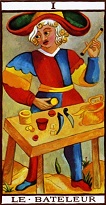
\includegraphics[scale=6]{a20121208MindFasting-img001.jpg}
\end{wrapfigure}

Intentional sacrifice then is training for concentration: we learn to distinguish the state of calm and freedom from the disorder of “desires, the imagination and discursive thought”. To be effortless, the will cannot oppose directly the sources of these disorders. Instead, we need to learn to detach from them, to observe them from a point of silence. Only then will they dissipate. This is the rational order of things, where the intellect is higher than, and dominates, thought and desire.

The season of Advent is the time of preparation for the incarnation of the Logos. Every physical event is the reflection of a spiritual reality and, since spiritual reality is timeless, it returns eternally. Hence, we can revisit the meditation on the second Arcanum as the Word is made Flesh.

There we see that the Logos is made incarnate by the Holy Spirit through the Holy Soul. As we are, the waters of our souls are full of perturbations. An event may create anger or anxiety, resulting in whirlpools that are hard to climb out from. There are tides coming in and out, so one day we say, believe, or vow one thing, and then the next day, just the opposite. Storms blow across the waters leaving them rough and choppy. In an unperturbed soul, the surface of the water is smooth line a pane of glass. Only in that condition will the Spirit be reflected clearly in the Soul. Otherwise, it gets mixed up with our fantasies and desires, which we too often take to be real expressions of the Spirit.

On the Feast of the Immaculate Conception we are reminded that only the Soul without sin can fully accept the Spirit. That Soul is totally free from perturbations. Can we even imagine what that is like? The exercise is worth the effort.

So either instead of, or in addition to, a physical fast, there is a Taoist exercise called mind fasting. If anyone has bothered to observe his thoughts, he will find abundant material to fast from. Perhaps there is a vulgar fantasy he indulges in. Perhaps he replays an event or conversations over and over in his mind. Perhaps he has a persistent anxiety or a worry. Maybe he has some daydream of success or power. Choose one and give it up. But give it up without effort.



\flrightit{Posted on 2012-12-08 by Cologero }

\begin{center}* * *\end{center}

\begin{footnotesize}\begin{sffamily}



\texttt{Senko on 2012-12-08 at 22:07 said: }

A most excellent post Cologero. Full of theory AND practical advice for one's everyday spiritual life. I find mental fasting much harder than physical fasting. I believe Advent is a most excellent time to prepare ourselves for the birth of Christ in our Heart. Blessings in Christ and Mary!\footnote{\url{http://senkosmos.blogspot.com.ar/}}


\hfill

\texttt{Mihai on 2012-12-09 at 14:43 said: }

Great post ! 

I would say that fasting has three different levels on which it must occur (like everything in the spiritual life, for that matter).

1. Physical: this is known by everyone and, unfortunetly, this is where it begins and ends in the mundane mentality of our age.

2. Psychic: just what you described here as “mind fasting”.

3. Spiritual: Without increasing prayer, meditation, study of Scripture etc. the whole thing collapses without purpose. 

I believe that when the fast turns into a petty legalism, limited to abstaining from certain foods and drinks, while ignoring the other two parts, it becomes even diabolical in character. I have seen a lot of people who do nothing but a physical fast and are most irritable and agressive during such a period.


\end{sffamily}\end{footnotesize}


\chapter{Memory}
\section{Immoral Dilemmas}

These are the results of my first experiments in remembering. Behind the temporal succession of the events of life, there is an eternal principle that gives them meaning and an intemporal I that is unchanged throughout.

The common view is that memory has something to do with the past, as when friends or family get together to relive their common nostalgic moments. Phenomenologically memory is bringing the past into the present. Or to put it another way, the seemingly disparate and unrelated events of life cannot be understood as merely temporal succession. As Rene Guenon expressed the goal in \emph{Oriental Metaphysics}:

\begin{quotex}
The person who attains this “primordial state” is still only a human individual and is without effective possession of any supra-individual states; he is nevertheless freed from time and the apparent succession of things is transformed for him into simultaneity. He consciously possesses a faculty which is unknown to the ordinary man and which one might call the “sense of eternity.” This is of extreme importance, for whoever is unable to leave the viewpoint of temporal succession and see everything in simultaneity is incapable of the least conception of the metaphysical order.

\end{quotex}
The exercise in remembering should lead to seeing one's life in its simultaneity. The events in their totality suddenly reveal a hidden meaning to life. This meaning is constant, eternal, and above time. What follows are some notes from this exercise. Keep in mind that there are four levels of memory of increasing depth:

\begin{enumerate}
\item \textbf{Intellectual memory}. The unadorned memory of a past event. 
\item \textbf{Emotional memory}. A memory that elicits an emotional reaction. 
\item \textbf{Volitional memory}. A memory that incites to action. 
\item \textbf{Moral memory}. A moral aspect is added to the memory. 
\end{enumerate}
Forgetting is analogous to death so remembering is life giving. Some memories arise spontaneously. Others take some effort. One should not stop at intellectual memory. It may take more effort to expand that memory to deeper levels. This essay has been some time in planning. The events mean nothing to you, but each time I've relived them, there is more intensity. Humor may be used to hide it. Nevertheless, over time, a common thread has been revealing itself to me.

You can avoid remembering now, but your entire life will be exposed at death. There is no point in evading the inevitable.



\flrightit{Posted on 2021-02-12 by Cologero }

\begin{center}* * *\end{center}

\begin{footnotesize}\begin{sffamily}



\texttt{Michael M on 2021-02-12 at 10:09 said: }

When it comes to viewing memories and the addition of the moral element and a common thread throughout life, the more we untangle those knots looking back and going further and further long those lines does give a different type of perspective or Gestalt of the whole. 

Utilizing that theme, would it be more advisable then to look at present / future events in the light of such a theme? Or is that too close to trying to get a specific result from a type of effort? Thereby destroying the whole effort to begin with. The building of a foundational “center” with a common theme that has always been present in life would reasonably seem to be the only true way to have a viewpoint or post for life that would never be carried away by external influences.


\hfill

\texttt{Tannheuser on 2021-02-12 at 13:24 said: }

““Say it, say it, say it.” Now I knew perfectly well what she wanted me to say, but I just couldn't say it. I was her one and only love but she was just one of many to me.

Tant pis pour elle. How much pain has unrestrained desire caused in the world? And why does it have to feel so good?”

—–

The girl who I couldn't “say it” to was actually the first woman I had ever slept with, and the most beautiful. Our relationship had started because I wanted to make the woman who I really loved at that time jealous, which worked. Still, for a while she sucked me into a world of immense pleasure that was hard to step away from. She had a very pleasing personality and the sex was incredible, but the whole thing was spiritually suffocating – I felt like Odysseus on Circe's island. 

In the end I only ever said “I love you” to three women, who corresponded in order to the types of ame-soeur, mistress, and wife.

—–

Michael M: If your life is a unity, then it only makes sense that you take action in the present from that perspective as you become conscious of your own meaning and purpose.


\end{sffamily}\end{footnotesize}

\section{The Persona and Ego}

\begin{quotex}
In the beginning the world was nothing but the Atman, in the form of a man. It looked around and saw nothing different
to itself. Then it cried out once, ‘It is I.’ That is how the word `I’ came to be. That is why even at the present day, if any one is called, he answers, ‘It is I,’
and then recalls his other name, the one he bears. \flright{\emph{Brihadâranyata-Upanishad}}

\end{quotex}
In \emph{The I Problem and Genius}\footnote{\url{https://www.gornahoor.net/library/IProblem.htm}}, \textbf{Otto Weininger} writes about the realization of the sense of the “I”, that
is, the experience of being an independent centre of awareness. Here are some descriptions he provides:

There has been no famous man who, at least some time in the course of his life, and generally earlier in proportion to
his greatness, has not had a moment in which he was absolutely convinced of the possession of an ego in the highest
sense. Let us compare the following utterances of three very great geniuses. \textbf{Jean Paul} relates in his
autobiographical sketch, \emph{Truths from my own Life}:

\begin{quotex}
I can never forget a circumstance which, so far, has been related by no one – the birth of my own self-consciousness,
the time and place of which I can tell. One morning I was standing, as a very young child, at the front door, and
looking towards the wood-shed I suddenly saw, all at once my inner likeness. `I’ am ‘I’ flashed like lightning from the skies across me, and since then has remained. I saw myself
then for the first time and for ever. This cannot be explained as a confusion of memory, for no alien narrative could
have blended itself with this sacred event, preserved permanently in my memory by its vividness and novelty. 

\end{quotex}
\textbf{Novalis}, in his \emph{Miscellaneous Fragments}, refers to an identical experience:

\begin{quotex}
This factor every one must experience for himself. It is a factor of the higher order, and reveals itself only to higher
men; but men should strive to induce it in themselves. Philosophy is the exercise of this factor, it is a true
self-revelation, the stimulation of the real ego by the ideal ego. It is the foundation of all other revelations; the
resolution to philosophise is a challenge to the actual ego, to become conscious of itself, to grow and to become a
soul. 

\end{quotex}
\textbf{Schelling} discusses the same phenomenon in his \emph{Philosophical Letters upon Dogmatism and Criticism}, a
little known early work, in which occurs the following beautiful words:

\begin{quotex}
In all of us there dwells a secret marvelous power of freeing ourselves from the changes of time, of withdrawing to our
secret selves away from external things, and of so discovering to ourselves the eternal in us in the form of
unchangeability. This presentation of ourselves to ourselves is the most truly personal experience upon which depends
everything that we know of the supra-sensual world. This presentation shows us for the first time what real existence
is, whilst all else only appears to be. It differs from every presentation of the sense in its perfect freedom, whilst
all other presentations are bound, being overweighted by the burden of the object. Still there exists for those who
have not this perfect freedom of the inner sense some approach to it, experiences approaching it from which they may
gain some faint idea of it. … This intellectual presentation occurs when we cease to be our own object, when,
withdrawing into ourselves, the perceiving self merges in the self-perceived. At that moment we annihilate time and
duration of time; we are no longer in time, but time, or rather eternity itself, is in us. The external world is no
longer an object for us, but is lost in us. 

\end{quotex}
Finally,

\begin{quotex}
Every great man knows this phase of the ego. He may become conscious of it first through the love of a woman, for the
great man loves more intensely than the ordinary man; or it may be from the contrast given by a sense of guilt or the
knowledge of having failed; these, too, the great man feels more intensely than smaller-minded people. It may lead him
to a sense of unity with the all, to the seeing of all things in God, or, and this is more likely, it may reveal to him
the frightful dualism of nature and spirit in the universe, and produce in him the need, the craving, for a solution of
it, for the secret inner wonder. But always it leads the great man to the beginning of a presentation of the world for
himself and by himself, without the help of the thought of others. 

\end{quotex}
\textbf{Miguel Serrano} has his own take on this in \emph{Nos: Book of the Resurrection}.

\begin{quotex}
Where is this persona when the child still has no sense of the individual “ego”? In my case, I remember, when I was a
year old or perhaps less, I was leaning out of a tower holding my grandfather's ring tightly in my hand.
The women of the house ran to take hold of me, because they were afraid that I would let it drop. But, I remember, that
child felt itself to be a persona, it knew the importance of the ring and knew that it would never let it drop. It felt
deeply offended by this lack of trust. That child was a very old and wise man. And when the “ego” became defined, it
was a philosopher who asked himself the question. That is the difference, I believe … and this is the ring. I have
recovered it. 

\end{quotex}

\flright{\itshape Posted on 2018-05-31 by Cologero}

\begin{center}* * *\end{center}

\begin{footnotesize}\begin{sffamily}

\texttt{Lyon on 2018-06-01 at 20:58 said:}

“But, I remember, that child felt itself to be a persona, it knew the importance of the ring and knew that it would
never let it drop. It felt deeply offended by this lack of trust. That child was a very old and wise man.” Miguel
Serrano

I recall having a somewhat similar realization around 4 years old, where I was clearly older, maturity-wise, than my age
would betray.

\hfill

\end{sffamily}\end{footnotesize}

\section{Birth of the “I”}

In \emph{The I Problem and Genius}\footnote{\url{https://www.gornahoor.net/?page_id=12944}}, Weininger writes about the realization of the sense of the “I”, that is, the experience of being an independent centre of awareness. He proceeds to give examples (from Jean Paul, Novalis, and Schelling) where they describe their earliest experiences “of the possession of an ego in the highest sense.”

Some men seem to have had a strong experience of that, often from an early age, while others don't even seem to understand the question. Readers may want to consider this an exercise in self-realization and try to remember their own such experiences. Here are two of mine:

\begin{quotex}
The first shocking memory I recall is when I had just finished a BM. I opened the bathroom door and called to my mother to take a look at it in the bowl. I was dumbfounded when she did not want to look at it and told me to go flush it myself. At that moment I woke up to myself and realized I was on my own.

\end{quotex}
That had to have been around two and a half years old. The following one was probably a year later:

\begin{quotex}
I tied all my toy trucks and cars together and made a train. As I pulled it around the house, my sister was crawling behind the train and following it. This is my first recollection of the sense of having a “will”.

\end{quotex}


\flrightit{Posted on 2008-07-06 by Cologero }

\section{Thanks for the Memories}

\begin{quotex}
you must know, Sancho, if you do not know it already, that with lovers, the external actions and movements, revealed when the topic of their love arises, are reliable messengers bringing the news of what transpires deep in their souls. \flright{\textit{Don Quixote}}

\end{quotex}
Memory is not mere reminiscing, but is a progress from the past to the present. In Bergson's diagram, the base AB of the inverted cone is the memory. The Self S lives and acts on the plane P, bearing the weight of the past. If you forget your past, you will be driven by unconscious forces. Memory is real and actual only in the present, to the extent that it shapes our perception and understanding of the world.

Plato famously claimed that knowing is remembering. In particular, we have forgotten the world of essences, that is, the ideas in the mind of God; Hence, knowing an essence is just a recall of that which was forgotten. A fortiori, knowledge of the Self, our essence, and our destiny must also be a form of remembering. But memory of the forms takes place in stages. We understand more as we rise up through the states of being. Boris Mouravieff explains:

\begin{quotex}
\emph{Memory} is a direct function of the \emph{being} of the individual. The higher the level of \emph{being}, the better the memory and the greater its capacity to contain. Loss of memory, which causes the notion of the name and the ensemble that is attached to it to be forgotten, makes a madman out of a normal man: the sense of continuity is no longer present. 

\end{quotex}

\begin{wrapfigure}{rt}{.25\textwidth}
\centering
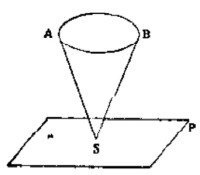
\includegraphics[scale=.5]{a20210131ThanksfortheMemories-img001.jpg} 
\caption{Memory Cone}
\end{wrapfigure}

The esoteric teaching is that forgetting is analogous to sleeping and to death, as they manifest on different levels. Valentin Tomberg makes it clear:

\begin{quotex}
For our whole experience (outer and inner) forgetting, sleep and death are three manifestations of the same thing —namely the “thing” which effects disappearance. It is said that sleep is the younger brother of death. It is necessary to add: forgetting is the brother of sleep. … One forgets, one goes to sleep, and one dies. One remembers, one awakes, and one is born. Remembering is to forgetting as awakening is to falling asleep, and awakening is to sleeping as birth is to death. … Natural forgetting reduces man to animality; natural sleep reduces him to vegetality; and natural death reduces him to minerality. 

\flright{\textit{Letter XIII, Death}}

\end{quotex}

Yet remembering is not simply bringing an image of the past into the present, since there are levels of depth to memory. You can remember solely with the intellect, with feelings, or even with the will. The highest is moral memory, based on love and all that accompanies it. Tomberg emphasizes the importance of the latter:

\begin{quotex}
It is love which is at work in moral memory when it recalls things from the past. Here it is admiration, respect, friendship, gratitude, affection and a thousand other things which have deeply moved you, which render things from the past unforgettable, i.e., evocable at each instant. The more one has loved, the more one remembers through moral memory.

Moral memory — which can comprehend everything without exception — is all the more effective the less one is morally indifferent. Indifference, a lack of moral interest, is the fundamental cause of the lapse of memory which often takes place in old age. The less one is indifferent, the more one remembers of the past and the more one is capable of learning new things. 

\end{quotex}
\paragraph{Moral Memory}
Moral memory predominates in old age. The young depend on mechanical memories, which arise spontaneously; this faculty becomes feebler with age. Hence, it must be replaced with intellectual or logical memory. This requires an active effort to remember things. People who neglected to learn how to make intellectual efforts in their youth, will become forgetful as they age. Tomberg goes even further, explaining that moral efforts are likewise necessary:

\begin{quotex}
People who are able to and who know how to give everything a moral worth and to see a moral sense in everything will not forget anything: they will have a normal, if not excellent, memory to a very advanced age.

Moral memory — which can comprehend everything without exception — is all the more effective the less one is morally indifferent. Indifference, a lack of moral interest, is the fundamental cause of the lapse of memory which often takes place in old age. The less one is indifferent, the more one remembers of the past and the more one is capable of learning new things. 

\end{quotex}
\paragraph{Love and Work}
\begin{quotex}
Love and work are the cornerstones of our humanness. \flright{\textsc{Sigmund Freud}}

\end{quotex}
To begin the experiment of “remembering”, one must first decide what to remember. If love and work are the cornerstones of our humanness, that is the place to start. When one loves, one cannot be morally indifferent. And our acts — our work, our projects, our adventures — only have significance when they are moral acts. So we turn to our favorite Knight Errant, Don Quixote, who had expertise in both realms, as a model.

Love was constantly on his mind, especially for the one special lady, who was the driving force, the creative force, for his life. He treated women with chivalry. Against men, he was prepared to do battle against iniquity and to protect the weak and helpless. He brandished his cold weapons to make a point. He did not carry around a copy of the constitution nor did he propose to reason with his enemies to make his point. That is why his deeds have been recorded and are remembered.

\paragraph{Pointillism}
Most people live their lives as an accumulation of points, one after the other. Events in their lives are unrelated to each other since points are unrelated. They are stuck in time and not in simultaneity. If you desire to live your life as a work of art, whom would you commission to paint it for you?

The realist will plan it in advance: he will make a detailed drawing, calculate the perspectives, choose the colours, lighting, etc. The end result is known even before the artist begins. The unsophisticated viewer prefers realism because it requires little or no effort from him.

The better choice is pointillism. As you live your life day to day, it is difficult to grasp it as a whole. Instead, your life appears to you as a series of points of various colours, almost at random, and it may not make sense as a whole at any given time. However, as the points are painted at various spots on the canvas, gradually the full image of your life can be discerned. But this takes more effort — and patience — by the viewer to wait for the points to begin to make sense.

So that is how to start, each memory is a point or set of related points. Over time, as they appear on the canvas of your life, the whole picture of your life should come into view.

\paragraph{Life is Short}
They say that life is too short. Your memories should be relevant; they should be predominantly moral memories. If your fondest memories are watching TV or hanging out at the pub, then your life is actually too long and you are trying to fill it up with trivialities.

To develop a moral memory, you must live by principles and your acts must have a point. This should be obvious, for the alternative is live a life that is unprincipled and pointless.

\paragraph{Dislikes, Fears, and Accidents}
The first step in deep remembering is to ascertain one's earliest likes, talents, and proclivities. This exercise is preferable to most people because it seems pleasant. However, one can gain more self-knowledge by remembering the things you did not like. What events transpired in your life that you did not desire? Can you see what role, however subtle, you may have played in bringing it about?

This applies also to what you most fear. How has the avoidance of this fear shaped your life?

Another consideration is to remember everything that occurred, seemingly by chance or accident. From the human point of view, that may seem to be the case. But can you dig even deeper to see if there is a state of being from which you willed those events.

Meditations like these will often bear great fruit.

\paragraph{Encounters with Others}
Your life is a world line in the cosmos. And everyone else has his own world line. Mathematically understood, a Point is where two Lines intersect. In other words, the points don't define the line, but the line defines the points that constitute it.

So when I see a Point, I don't ask what it means in isolation. Instead, I look for the two lines. Of course, you are one of them, and the other is a person you encounter. Why are two distinctly different world lines meeting at that point? From that perspective, you can experience the event in its wholeness, all at once, simultaneously.

There are natural reasons, of course, for the intersection of lines: family, jobs, food, love, revenge, and so on, i.e., all the things involved in human life. But that does not exhaust all the possibilities.

Nevertheless, some lines meet for no human purpose at all, yet you can't dismiss it as pointless because the Point is there and is unavoidable. You may choose to look away. That is possible because it is so ethereal. But that decision has its danger, since you may miss one of the most important moments in your life.

How many of those life events have you forgotten? and you may even be glad they are forgotten. How few of those memories will endure through eternity? It is imperative to know what to forget and what to remember.

Why have some people made an impact on your life and others not so much?

\paragraph{Things forgotten}
You will find memories best left forgotten. Something that had seemed so important and so impactful at that time, appears now in retrospect to be so distant, so far from your current level of being, that it may as well have been the memory of a different person. It may remain as an intellectual memory, but it no longer has any emotional impact, and it most certainly does not induce you to act.



\flrightit{Posted on 2021-01-31 by Cologero }

\begin{center}* * *\end{center}

\begin{footnotesize}\begin{sffamily}



\texttt{Michael M on 2021-01-31 at 10:26 said: }

“They say that life is too short. Your memories should be relevant; they should be predominantly moral memories. If your fondest memories are watching TV or hanging out at the pub, then your life is actually too long and you are trying to fill it up with trivialities.

To develop a moral memory, you must live by principles and your acts must have a point. This should be obvious, for the alternative is live a life that is unprincipled and pointless.”

You describe exactly my experience lately when I hear someone say “killing time”. Internally I watch my cage intensely when I see it in others and am watchful for it in my own domain. Quite insidious a phrase especially when understanding time as part of the compound nature of experience, life, and the unfolding of ideas. Don't want to fall asleep in a dream and dream our life away…

Has anyone found it more difficult at times to remember “facts” (academic / intellectual) memories when focusing on moral memory intensely? Or perhaps there is some type of learning curve or displacement of useless knowledge for rewriting of moral orientation?


\end{sffamily}\end{footnotesize}

\section{Immaterial Intimacy and Material Catastrophes}

\paragraph{Introduction by Cologero}

\begin{quotex}
and directing his gaze from now, on towards beauty as a whole, he should turn to the great ocean of beauty, and in contemplation of it give birth to many beautiful and magnificent speeches and thoughts in the abundance of philosophy. \flright{\textit{Diotima to Socrates in Plato's Symposium}}

\end{quotex}
Diotima was a prophetess and philosopher. In the Symposium, she explains the ladder of love, which comprises the following stages.

\begin{enumerate}
\item In youth one Is attracted to the physical beauty of the other. 
\item At this stage, the spiritual beauty of another person is more important. Therefore, love is now directed towards this person because of her moral, intellectual, and spiritual qualities. 
\item The beauty of knowledge itself becomes the focus. This is the love of Wisdom, or philosophy. 
\item Ultimately, one reaches the appreciation of Beauty apart from any individual, to consideration of Divinity, the source of Beauty, to love of Divinity. 
\end{enumerate}
If Diotima is speaking as a philosopher, those stages make sense. But not if she is speaking as a prophetess of the future since precious few manage to get beyond the first stage. However, in the timeless realm, the notions of past, present, and future are relative. In the Future of Prophecy, Saint Gregory the Great\footnote{\url{https://www.meditationsonthetarot.com/the-future-of-prophecy}} explains the three tenses of prophecy: future, present, past:

\begin{quotex}
prophecy is not a matter of prediction, but rather of revelation. That is why there can be a prophecy of the past and the present; prophecy uncovers hidden truths, truths concealed by time or by present circumstances. He writes: “Prophecy is present when something is concealed, not by the spirit, but by the absent Word, which however is laid bare by the Spirit.” 

\end{quotex}
Sibylle has done her own experiment in making the past present, through the act of remembering. She had been working on those memories for a long time and until recently never figured out what to make of them. Suddenly, their meaning was revealed to her. That is how she became Sibylle.

You can find her experience in the New Decameron at Immaterial Intimacy and Material Catastrophes\footnote{\url{https://gornahoor.net/decameron/immaterial-intimacy-and-material-catastrophes/}}.

As you try your own experiment, notice the extent that you have contributed to the events of your life, whether out of ignorance, by accident, or deliberately.


\hfill

\paragraph{The Chewing Gum Boy}

She really didn't like the boys in Kindergarten. They constantly bullied her, said mean words, started laughing in her presence. There was one boy especially cruel, quite obscene for a five-year-old. Very blonde, strong and he kept singing Nena's “99 Luftballons” using a huge wooden building brick as a microphone. One day when she went to the supermarket with her mother, they encountered this boy with his mother. The two mothers started talking and he was too embarrassed to look at her. She didn't care because she thought she didn't like him. All of a sudden, the boy reached out and handed her a chewing gum. When he finally looked at her, she knew that cruel boys would never pose a danger to her. They revealed their true feelings by their first glance.

\begin{wrapfigure}{rt}{.3\textwidth}
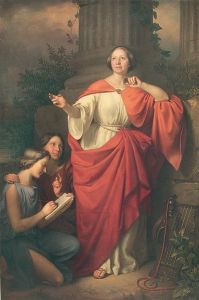
\includegraphics[scale=.5]{a20210215ImmaterialIntimacy-img001.jpg} 
\caption{Diotima}
\end{wrapfigure}

\paragraph{Ending up in the Boys Corner}
On her first day of elementary school, the girls of her class promised each other to stick together in order to avoid sitting next to a boy. When the teacher announced everybody should choose a seat, her best friend ran away to sit with another girl. So she picked a nice window seat next to a long-haired, fair looking girl. Suddenly the girls started laughing at her. When she looked around, she realised she was surrounded by boys. The fair looking girl turned out to be a boy — she spent the rest of the schoolyear by his side, but never figured out what he was either thinking or feeling. He remained completely alien to her.

\paragraph{The Teacher}
When she was thirteen, she switched violin teachers. Her father had taught her since she was four and made his daughter the winner of a several local music competitions. Now that she was supposed to win the national youth competition the stakes were high. A new coach was needed: a motivating, inspiring presence who would make her leap to the next level. The Teacher was indeed motivating and inspiring — mainly because she was terribly in love with him. She would have lessons at his home, eat lunch with his parents — he only touched her slightly, she told me that it felt like a breeze on her neck and arms. So she won the competition, everyone was happy except for her. Why? The Teacher was a decent man: winning was nice — but she wanted Love.

\paragraph{Love gone unnoticed}
After she dropped out of High School when she was 17 to advance her career, she went on a concert tour in the Czech Republic with two very sweet boys, a cellist and a pianist. They were part of a group of prizewinners of an international music competition playing concerts in Prague and Bohemia. She fell in love with the pianist, spent her evenings kissing him and enjoyed herself until one morning she discovered the ashes of a letter on the doorsteps of her motel room. She had no clue what that was all about. It turned out that the cellist had fallen in love with her, planned to open up to her in a love letter, but found out about her and the pianist. She hadn't noticed anything. She didn't feel sorry for him then. Maybe she does now.

\paragraph{The Tragedy of Napoli and Thanksgiving in Chicago}
During her first year at Indiana University, she met the Italian. He started calling her by his own last name as if they were already married. In fact they had barely exchanged a kiss. During the summer she went to visit him in Naples. Her parents had rented a house near Pisa for the holiday season and she took the train down to the South. She felt confident, had learned Italian in six weeks and was looking forward to meeting her future husband again. He was very passionate upon her arrival, but fell short of making love to her. Instead he called his best friend, a manic-depressive art student from Bloomington, who was spending his summer travelling around Italy. For the rest of her stay she spent more time with that best friend than with her supposed future husband. Back in Bloomington she kept hearing stories about him — that he had broken so many hearts, sleeping with every girl in town. Just not with her.

On Thanksgiving Day she decided to change the Matrix. Instead of letting things happen to her she allowed a student from Venezuela to take her virginity in a motel room in Chicago. He got mad at her for not telling him that it was her first time. She had simply assumed he wouldn't care and was stunned that he felt responsible for what she had made him do. Her first encounter with wrongly guided willfulness.

\paragraph{Mr. Nice Guy}
She did not love him at first. But she thought it was time to settle with a “nice” guy and found a seemingly willing partner in a German cellist she studied with in Amsterdam. They came from the same prude-protestant background and did everything right. Meeting both parents, spending time with his ersatz father — a highly skilled psychologist who kept emphasising how good she was for him after his ill-fated relationship with his former girlfriend. Still: he loved his ex-girlfriend and no other woman could make him happy. A couple of years ago the nice guy's ex-girlfriend committed suicide.

\paragraph{Another Change to the Matrix}
She tried another change to the Matrix. She felt trapped and pushed by external expectations and wanted to be left alone. So fifteen years ago she went online, picked herself a husband from a dating site, became pregnant and got married. Her husband was her best friend for a while. But he always seemed emotionally detached. When she finally managed to catch a glimpse of his Anima, she got scared. He was totally unaware of her. Everything she actively achieved by \emph{free movements} seemed like a catastrophe to her.

Some time ago he confessed to her that he is still trying to cope with his first girlfriend breaking up with him 35 years ago. If he had told her that fifteen years ago, she would have never married him.

So mere willfulness is not a strength in itself? I think she knows that by now. She has tried to change the Matrix twice and just created a Matrix inside the Matrix.

\paragraph{Sybil}
I was conceived spontaneously. Almost accidentally, not willingly. I could have remained silent forever. I don't know why I didn't. She made me write and delete and then rewrite a comment before eventually sending it. She wasn't really expecting an answer, she was just fed up with the passivity of men in her life, had a weak moment and made me comment on some really beautiful and deep thoughts on Love.

But when I think about it — there was more to it than her weakness. She was intrigued by the thought that skin would become an obstacle to intimacy. Since she had experienced her most intimate moments with little or no physical contact throughout her life, she seemed puzzled by the idea that this could actually be a Path and not a flaw.

Me: But you used to be so sceptical of Diotima's talk.

Her: Yes, but that was before.

Me: Before what?

Her: Before he listened to what I meant instead of what I said. He didn't close the door even if he really wanted to. But he said “Stay with me” instead. By knowing me better than I knew myself he acted like a true Knight.

Me: Now you sound like an overly romantic scriptwriter.

Her: It's better than watching the same old film over and over again.



\flrightit{Posted on 2021-02-14 by Sibylle }


\chapter{Remembrance of death}
\section{Death and the Real I}

\emph{If we keep the image of death constantly in our minds, we will appreciate with bitter regret the value of each lost day.}

\paragraph{Dark Dream}

\begin{wrapfigure}{rt}{.3\textwidth}
\centering
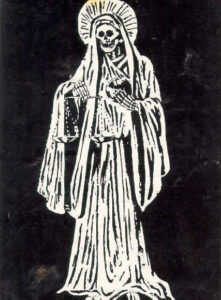
\includegraphics[scale=.5]{a20191027DeathandtheRealI-img001.jpg} 
\caption{Muerte Blanca} 
\end{wrapfigure}

I was driving on the highway at night, paying close attention to the traffic. A cop car ahead of me, a few cars in the lanes to my left. I accidentally turned off my headlights but could not turn them back on. Suddenly, the entire highway was pitch black. I continued to drive, unable to see anything ahead. The brakes did not work, yet the car was accelerating. I was weaving in and out, all the time thinking that I would crash into something. I speculated on what crash would occur while continuing to drive.

The ambiguity was clear. Was I heading into the darkness of death? Or was I being guided by unknown forces?

In Chapter V of \emph{Gnosis} Book 1, Boris Mouravieff includes a meditation on death, which comprised three exercises. The I of the Personality gives little thought to its own death. Mouravieff explains:

\begin{quotex}
All man can imagine in this respect is to evoke the image of his own corpse: he can never exclude from this representation the observer who contemplates this image. 

\end{quotex}

Only the Real I can contemplate one's death. While the ego looks for the light, the Real I faces the darkness. In most cases, it takes a major event, a boundary situations, to get the ego to face its own annihilation. Examples are: fright, guilt, finality, and suffering.

\begin{wrapfigure}{rt}{.3\textwidth}

\includegraphics[scale=.4]{a20191027DeathandtheRealI-img002.jpg} 
\end{wrapfigure}

\paragraph{Exercise 1: Remembrance of death}
\begin{quotex}
Death is the only real and unique event which happens to us without fail. In other words, constantly bearing in mind the idea of death approaching nearer every day is a concrete means of facing an implacable reality — before which all the joys and all the worries of the Personality fade. It is thus that one learns that in effect: `all is vanity and torments of the mind.' 

\end{quotex}
It is insufficient to read this exercise; rather, one must actually do it. The timing is good. During Halloween season in the USA, people decorate their lawns with images of death. Walk around the neighborhood and contemplate the skulls. It is better than candy.

This week: pray for the dead and visit a cemetery.

\paragraph{Exercise 2: The narrow road leading to Life}
\begin{quotex}
This is done by introducing a continuous and permanent attachment between the Personality and the passive Real `I'. so as to render the presence of the latter constant in the field of action of the Personality. Then, with time and according to the intensity of efforts, the situation can undergo a complete change: the more the Real I – like the grain of mustard seed – takes root in the mental life which was until then dominated by the Personality, the more the latter is subjected, little by little, to the will of the judge. Identifying himself with it, man will rediscover his Real `I' in all its integrity and permanence. For him, life then loses its factitious character, to become logical and factual. 

\end{quotex}
Train the ego, or false I, to become aware of the Real I. The ego lies to himself; it sugarcoats his life. The Real I judges rightly, which the ego dislikes. Ultimately, the goal is for the ego to become passive to the Real I. Learn to distinguish between the speech of the ego and the Real I.

\begin{quotex}
When a person speaks, it is generally easy to distinguish whether his records are playing or whether he speaks from some deeper part of himself. In the latter case, he uses a pictorial, rustic and sometimes awkward language; in the former he speaks in a singing tone of voice. 

\end{quotex}
\paragraph{Exercise 3: The philosopher's stone}
\begin{quotex}
The permanent link which must be introduced between the Personality and the real `I' is esoteric Knowledge. The knowledge and know-how that it permits us to acquire represent the philosophers' stone of the medieval mystics. They are capable of provoking in man the transmutation to which he aspires. 

\end{quotex}
Read the best material rather than wild speculations or useless opinions.

\paragraph{Summary:}
\begin{itemize}
\item Constantly bear in mind the idea of your own death 
\item Make the real I the master of the I of the Personality 
\item Acquire esoteric knowledge 
\end{itemize}
\paragraph{Leaving the I of the Personality Behind}
\begin{quotex}
the petty bourgeois is spiritless[.] … Devoid of imagination, as the petty bourgeois always is, he lives within a certain orbit of trivial experiences as to how things come about, what is possible, what usually happens, no matter whether he is a tapster or a prime minister. This is the way the petty bourgeois has lost himself and God. \flright{\textsc{Soren Kierkegaard}, \emph{The Sickness Unto Death}}

\end{quotex}


\flrightit{Posted on 2019-10-27 by Cologero }

\begin{center}* * *\end{center}

\begin{footnotesize}\begin{sffamily}



\texttt{Patricia on 2019-10-28 at 17:05 said: }

Your dream reminds me of the dark night of the senses that St. John of the Cross wrote about. The gift on the other side of that “night” erupts in the last sentence of your writing, concerning the moments when joy and beauty suddenly appear. I am so glad you made it through such a difficult medical and spiritual challenge.


\hfill

\texttt{Santiago on 2020-10-28 at 13:16 said: }

One of my favorite articles on the site. Steps 2 and 3 seem somewhat more difficult!

Regarding step 1, Evola states in Doctrine of Awakening, that it's a good practice to witness an autopsy and meditate on the nature of death. The idea being, if I recall correctly, to maintain an awareness that we are more than our physical body. There are many autopsies one may watch on YouTube, and all are quite grotesque, so squeamish viewers should overlook the provided example: https://www.nsfwyoutube.com/watch?v=nHeFUT-11So (NSFW)

“Only the Real I can contemplate one's death. While the ego looks for the light, the Real I faces the darkness. In most cases, it takes a major event, a boundary situations, to get the ego to face its own annihilation. Examples are: fright, guilt, finality, and suffering.”

Is the sensation of ego annihilation typically accompanied by a `deep' darkness and a profound, rapid sense of `falling'. I had this experience recently, and it was so overwhelming that I impulsively stood up and gasped for air, ending immediately the experience.


\hfill

\texttt{Greg on 2020-10-29 at 14:24 said: }

Is death the annihilation of the personality? If you listen to nde accounts it would seem not but I suppose they might be unreliable.


\end{sffamily}\end{footnotesize}


\chapter{Sparse notes and some guides to life}
\section{Amor Fati and the Heroic Life}

\begin{quotex}
My formula for the greatness of man is amor fati — to change nothing, neither before nor after, throughout all eternity. Not only to bear Necessity, and still less to hide it — all idealism is a lie in the face of Necessity — but to love it. \flright{\textsc{Friedrich Nietzsche}}

A happy life is impossible; the highest to which man can attain is an heroic course of life. \flright{\textsc{Arthur Schopenhauer}}

\end{quotex}
\paragraph{Amor Fati}
The highest form of Amor Fati is to follow the will of God. The first act of will is the acceptance of the circumstances of your birth. To wish it to have been otherwise, is to wish to have been someone else.

When \textbf{Saint Anthony the Great} thought about the depth of the judgments of God, he asked,

\begin{quotex}
Lord, how is it that some die when they are young, while others drag on to extreme old age? Why are there those who are poor and those who are rich? Why do wicked men prosper and why are the just in need? 

\end{quotex}
He heard a voice answering him,

\begin{quotex}
Anthony, keep your attention on yourself; these things are according to the judgment of God, and it is not to your advantage to know anything about them. 

\end{quotex}
\paragraph{The Heroic Life}
To resist the modern world, embrace what is most despised by the modern world and, a fortiori, also despised by some who fantasize about resistance. Embrace the world that valued:

\begin{itemize}
\item Logic, grammar, rhetoric 
\item Geometry, mathematics, music, cosmology 
\item True philosophy in the mould of Plato and Aristotle 
\item Mysticism 
\item Chivalry 
\item Art, Poetry, Architecture 
\item Social Order 
\item Care widows, orphans, the sick, and infirm 
\end{itemize}
Dante showed the path from the bug life (mere animation) to Union with God. The seven stages are described in their all-too-human detail, not as some lifeless abstractions. This path will lead to results and save you years of fruitless seeking. Do not just read, but actually apply, what is contained in these texts:

\begin{itemize}
\item \textbf{Richard of Saint Victor}, \emph{De Contemplatione} 
\item \textbf{Saint Bernard}, \emph{De Consideratione} 
\item \textbf{Saint Augustine}, \emph{De Quantitate Animae} 
\item \textbf{Saint Thomas Aquinas}, \emph{Summa Theologiae} 
\item \textbf{Dante}, \emph{The Divine Comedy} 
\end{itemize}


\flrightit{Posted on 2020-08-07 by Cologero }

\section{Last Word}

The next task is also the last task and therefore the most difficult one. Four things are necessary to fulfil it.

\paragraph{Live by Principles}
Research the principles of \textbf{Bernard of Clairvaux} for a good life and live by them.

That has been your task from the start. Everybody forgot. Do not forget that amongst these principles most important one is to pledge your life and everything that one owns to the cause, defence, honour and further knowledge of the Christian religion and the Holy Church. That means both Catholic and Orthodox Church each with their own dogmas and respective holy centres and patrons. Neither defamation nor furthering of the schism belongs to the life one has been expected to lead. This task also does not have anything to do with common modern day politics and enmities, daily life and journalism, as such are regarded to be realities of a profane nature, so one should relinquish any attempt to conjoin your task with latter. Such is permittable only in one case, that of utmost necessity and solely that — indeed the same you have been called up for — defence, honour and further knowledge of the Christian religion and the Holy Church.

\paragraph{Basic Training}
To be able to live up to these principles, you need to acquire a basic training.

The first steps are: the control of thinking, feeling, willing, control of speech, control of action, all these combined. Not in a 10 minute meditation, not in an exercise, one is also not expected to perfect this as everybody comes to a situation sooner or later where one fails this and shows weakness and doubt. In such situations remember also that Our Lord suffered in Gethsemane, find strength in remembering that nevertheless he completed his Mission in the end for all of us. Try then to accomplish what is asked from this training in situations when it is needed and important.

Correct thought, correct feeling, correct word, correct action.

\paragraph{Mutual Respect}
Observance and Excellence, Education and Culture, Ethics and mutual Respect of other Confessions, as well as always when necessary and possible, mediating a peaceful dialogue between them; furthermore, abiding all written and unwritten laws and mores, national and International — is what is asked from all who decide to follow this path. To achieve these, one should school oneself also in the art of oratory — as a proper expression — so that a man can be considered wise and truthful whether with friends or in the face of adversary, and at both tables he will be respected and well received.

\paragraph{Service}
All these you must not do to excel and take pride in your achievements when you compare yourself with your neighbour. You do all this to serve. Christ washed the feet of his disciples and he was the First among all. Love your neighbour\footnote{Updated 13 IX 2020.

This is the last task assigned to me by a dear spiritual friend. As for the materials sent to me, I have been using them, not always explicitly. Those who are supposed to manage them, can't manage.

But I need to improve German vocabulary so I don't get slowed down looking up words.

As for oratory, I have new audio equipment. But it seems a lot of work for little reach. I'm not Joe Rogan.}.



\flrightit{Posted on 2018-09-13 by Anon }

\begin{center}* * *\end{center}

\begin{footnotesize}\begin{sffamily}



\texttt{Cologero on 2018-09-13 at 22:18 said: }

Very moving, but we have to take into account human capacities. For example, you alluded to some exercises suggested by Rudolf Steiner. As he points out, however, even 10 minutes may be too strenuous for most people. In \emph{Knowledge of Higher Worlds}, he makes this suggestion:

\begin{quotex}
The student must set aside a small part of his daily life in which to concern himself with something quite different from the objects of his daily occupation. The way, also, in which he occupies himself at such a time must differ entirely from the way in which he performs the rest of his daily duties. But this does not mean that what he does in the time thus set apart has no connection with his daily work. On the contrary, he will soon find that just these secluded moments, when sought in the right way, give him full power to perform his daily task[s]. Nor must it be supposed that the observance of this rule will really encroach upon the time needed for the performance of his duties. Should anyone really have no more time at his disposal, five minutes a day will suffice. It all depends on the manner in which these five minutes are spent. 

\end{quotex}

\hfill

\texttt{Anon on 2018-09-14 at 03:19 said: }

When you finish the material I sent you, tell me what you think about then about this same matter. Who cant manage, cant manage. Things are how they are.


\hfill

\texttt{Cologero on 2018-09-14 at 12:22 said: }

Well, Anon, if I have to finish the material first then you have not yet said the Last Word.

The goal is to help serve others (i.e., those who read this blog), as you wrote, not to display one's own superiority.

So let's discuss Steiner's exercise from a book that you recommended to me as part of the “material”. Why do suppose that 5 minutes do not suffice?

The material also includes this passage:

\begin{quotex}
Pay attention to your ideas. Only think important thoughts. Learn to separate in your thoughts the essential from the inessential, the eternal from the transient, the truth from mere opinion.

When listening or talking to one's fellow man, one tries to become completely silent within oneself and to give up all approval, in particular all disparaging judgments, both in thoughts and feelings. 

\end{quotex}
Does that mean we should withhold disparaging judgments, at least until we are sure we understand?

How does one separate the eternal from the transient? Certainly comparing the human condition from 800 years ago to day might be a prelude to that.

When we consider correct speech, the circumstances need to be taken into consideration. What is appropriate in one setting may not be in another. And when is it necessary to speak out? Would it not be correct speech to point out crimes and injustice? Silence is Consent: \textit{Qui tacet consentire videtur, ubi loqui debuit ac potuit}.

You may have forgotten Point 5: forgiveness. Things are not simply how they appear, as you imply. A person does not acquire all those qualities on a balmy weekend. It is the task of a lifetime, and there will be failures on the way, many failures. Forgiveness ought to follow faults, but it seems to be much easier to err than to forgive.


\end{sffamily}\end{footnotesize}

\section{The Greatness of the Soul}

In \emph{De Quantitate Animae}, the \emph{Greatness of the Soul}, Saint Augustine describes a path that leads the soul from “its vivifying, perceptive, rational and contemplative powers that enable it to move close to God”. It is Augustine's understanding of the seven stages of the ascent to God. This work served as one of Dante's main influences.

This path is certainly consistent with other descriptions, so I have modified the names of some of the stages for clarity. It cannot be emphasized enough, this is not theory. In other words, these stages can be experienced, a fortiori, they must be experienced in order to be properly understood.

\begin{enumerate}
\item Animation 
\item Sensual Life 
\item Rational Life 
\item Autarky 
\item Ataraxia 
\item Theoria 
\item Theosis 
\end{enumerate}
\paragraph{Animation}
This refers to the vegetative soul, common to all life. Its characteristics are the nutritive, growth, and reproduction functions. Plants, fungi, and perhaps some lower animals have only the vegetative soul. It lacks consciousness. For higher beings it is the source of will and desire.

\paragraph{Sensual Life}
The sensitive or animal part of the Soul includes the powers of perception, sensation, and (willful) movement. It includes the external (sight, sound, smell, touch, taste) and internal (imagination, common sense, estimation, memory) senses. It is also the seat of emotions.

\paragraph{Rational Life}
While the vegetative and sensitive souls are connected to the operations of the body, the rational or intellectual soul exceeds the corporeal nature. As such, it is unique to human beings. Its functions are reason, knowledge of universals, ability to choose the good.

Since the rational soul is not a corporeal function, it cannot be natural; hence it is above nature. This, however, does not mean that there is no dependence on bodily functions or brains. It does mean that there is no natural process, e.g., genetics or neuronal activity, that cause the knowledge of universals or virtue. Specifically, it could not have “evolved” by any biological process.

\paragraph{Interlude on sensual and spiritual man}
\begin{quotex}
But the sensual man perceiveth not these things that are of the Spirit of God; for it is foolishness to him, and he cannot understand, because it is spiritually examined. But the spiritual man judgeth all things; and he himself is judged of no man. \flright{\textsc{1 Corinthians 2:14-15}}

\end{quotex}
The three aspects of the soul do not work harmoniously in humans anymore. People are centred predominantly in one of the three parts of the soul. Even the rational soul is used in service to the needs and activities of the body, not for higher things. These are the characteristics of the three types of sensual people.

\begin{itemize}
\item \textbf{Vegetative Soul}. This being is attached to sensations, thrills, sex, food, etc. They are usually men of action. His main fault is not using the will for higher things. 
\item \textbf{Sensual Soul}. This being is dominated by emotions, and reacts emotionally. He is likely to be sentimental or romantic. At its worse, he will be angry, malicious, anxious, etc. It is difficult to get him to think logically. 
\item \textbf{Rational Soul}. His focus is thinking, calculating, researching. He is on a constant search for the next big idea, the next book, where he believes he will find the ultimate answer. He will debate various verbal formulations. His fault is that he is unwilling to commit to a course of spiritual development; he would rather “know about” it rather than actually do it. 
\end{itemize}
Those embedded in the sensual life don't have a stable I, since it is driven by external factors: new experiences, emotions, new ideas. Most people prefer to live this natural life, unless some boundary situation or conversion experience pulls them out of slumber. At that point, they may be ready to embark on the true spiritual journey.

\paragraph{Autarky}
\begin{quotex}
It is necessary to be one in oneself (concentration without effort) and one with the spiritual world (to have a zone of silence in the soul) in order for a revelatory or actual spiritual experience to be able to take place. \flright{\textsc{Valentin Tomberg}}

\end{quotex}
Once a man has decided to transcend his natural life, the next two stages are critical. If he falters or fails at these stages, he will most likely be worse off than if he had never even begun a spiritual journey.

Autarky means to have dominion over one's soul. The consciousness of the natural man is driven by forces external to him, so his life is inconstant. The task, then, is to be able to concentrate on one's True Self. Then the psychological forces originating from below can be observed dispassionately. In the natural state, one's attention is hijacked by impulses, emotions, ideas, that arise spontaneously. In the concentrated state, one then learns to monitor and detach from such impulses.

Now, the rational soul can exercise its true function. No longer in submission to corporeal life, it turns to knowledge of the universals and virtue. The practice of the virtues, which is basically inner power, will lead to the strengthening of the I.

\paragraph{Ataraxia}
After Autarky has been achieved, attention can be directed from the world of the senses to the spiritual world. This requires the “Zone of Silence”, which is the reduction, or even elimination, of the perturbations of the soul. These include the automatic movements of thoughts, images, passions, personal desires, and so on. In other words, this is the purification of the mind and will.

Ataraxia is the inner state of tranquility and mental calm. Complete trust in God replaces trust in the world. When the soul is silent, then authentic spiritual experiences may take place.

\paragraph{Theoria}
This stage is inaugurated when interest in the things of the world is replaced by the desire of knowing what is true in the supreme degree. Meditation is the means. Once skilled in Concentration, Meditation is the next step. Learn to focus on an idea, or image, or some spiritual writing. Block off some time for it. However, you will find that, throughout the day, the meditation will spontaneously come back to you. You may even receive deeper insights about the object of meditation.

\paragraph{Theosis}
\begin{quotex}
Contemplation is the science of love, which is an infused loving knowledge of God, and which enlightens the soul, and at the same time kindles within her the fire of love, till she shall ascend upwards step by step unto God, her Creator, for it is love only that unites the soul and God. \flright{\textsc{Saint John of the Cross}, \emph{The Dark Night of the Soul}}

\end{quotex}
When even the words and images used in Meditation drop away, the next stage is contemplation. Saint Augustine describes it as the vision and contemplation of truth. As such, it is reason united with divine revelation. Tomberg describes it this way:

\begin{quotex}
Contemplation — which follows on from concentration and meditation — commences the very moment that discursive and logical thought is suspended. Discursive thought is satisfied when it arrives at a well-founded conclusion. Now, this conclusion is the point of departure for contemplation. It fathoms the profundity of this conclusion at which discursive thought arrives. Contemplation discovers a world within that which discursive thought simply verifies as “true”. 

\end{quotex}
This is why we insist that discursive thought is insufficient to understand the highest ideas of our Tradition. At best, discursive thinking gives the illusion of spiritual knowledge and at worse, it degenerates into a Wittgensteinian language game.

Beyond this, I am not in a position to explain more. That is reserved to the Saints that Dante places in the Empyrean: Augustine, Benedict, Francis. They should be your guides.



\flrightit{Posted on 2020-08-13 by Cologero }

\begin{center}* * *\end{center}

\begin{footnotesize}\begin{sffamily}



\texttt{Alan on 2020-08-14 at 01:05 said: }

“Detract not the king, no not in thy thought; and speak not evil of the rich man in thy private chamber: because even the birds of the air will carry thy voice, and he that hath wings will tell what thou hast said.” = unceasing silence.


\end{sffamily}\end{footnotesize}

\section{Our Thoughts Determine Our Lives}

Cologero had mentioned this book\footnote{\url{https://www.amazon.com/Our-Thoughts-Determine-Lives-Teachings/dp/1887904190}}, coincidentally, at the same time that I had stumbled across it myself, so I finally made the purchase, and finished reading it. I found it most helpful; Elder Thaddeus\footnote{\url{https://orthodoxwiki.org/Thaddeus_\%28Strabulovich\%29_of_Vitovnica}} is simultaneously very strict (insofar as he sets out an arduous teaching\footnote{\url{http://www.orthodoxengland.org.uk/pdf/thaddeus.pdf}}) and yet very compassionate, encouraging, and “human”: at one point, the man even had a cigarette problem, which he overcame, while in Kosovo at the Pech monastery. Elder Thaddeus was not a legalistic or judgmental man – what he was, most definitely, was a saint.

\begin{wrapfigure}{rt}{.3\textwidth}
 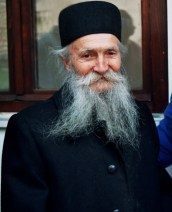
\includegraphics[scale=.6]{a20130412OurThoughtsDetermineOurLives-img001.jpg}
\end{wrapfigure}

Apparently, Elder Thaddeus had several experiences with angels, one while wide awake in prison, in which a very tall man wearing an old military uniform with a strange gold cross came to him to assure him that the Nazis would not be executing him, because God had many in Serbia that needed comfort. He also experienced the prayer “in” or “by” the heart through the Jesus prayer, and attained all three levels of Orthodox mystical experience by the time of his death. At his funeral, the birds, of whom he had often spoken with love and admiration, came in great numbers.

Here are some important points of doctrine gleaned from his essays, topical sermons, and quotes (ie., these are points that are repeated in various contexts and ways).

\begin{enumerate}

\item Man is a spiritual being who is dominated by psychic delusion and bodily passions, which convince us that “we” need something that is superfluous.

\item This domination always occurs through the power of aerial spirits, which are fallen angels, who have access to man's psychic constitution and long experience in manipulating man.

\item These spirits have varying degrees of wickedness, even among their own hierarchy.

\item They do this because they are lonely, fearful of the coming judgement, envious of man's special and privileged status, and because they also “feed” off the psychic energy derived from man's falling into sin. Each angel or spirit has their own “specialty”.

\item Man has the power to resist this, primarily because these spirits cannot access or even see man's inner heart, and because God Himself intervenes very frequently to lead souls back to Him.

\item God knew that the original state of man would “fall”, and that we would not be able to maintain our perfection; He therefore wisely and compassionately determined to use His own nature, and ours, in a synergistic way to overcome the fall, to lead back certain souls who remembered Him despite their sins, through their educative process back to a pristine condition.

\item This synergism is most boldly seen in the figure of Christ, who is the archetype or pattern for what will come after.

\item Mary the Theotokos is the pattern for what our love for God should be like. (I will speculate that this is primarily due to the lack of perfection in Christ, and the “feminine” nature of our soul in relation to its higher parts/God). Christ is the eventual pattern for our love, but Mary is chief among the saints.

\item Communion with angels and saints is necessary in order to achieve communion with God.

\item No evil spirit can touch someone who hasn't first harmed themselves. “We are the sole architects of our future”.

\item Everyone without exception desires absolute life and love: humans are variously warped in their search for this.

\item Vigilance, eternal vigilance, is necessary to achieve a state of grace, and even to keep it. You must examine every thought that enters your inner heart.

\item Only through the descent of the higher part of the soul, the Nous, into the heart, can a state of illumination be achieved. This state can be prepared for, and God will grant it, but only when the time is right (ie., when someone has a chance of keeping it, and/or not abusing it for evil ends).

\item Obedience and vigilance are greater virtues than fasting and even prayer, unless the prayer comes from the heart (or, greater, is “of” the heart).

\item God will listen to any prayer from the heart, even if someone is very far from Him.

\item The evil spirits try very hard to separate children from parents, because this fracture of Tradition and custom accomplishes the loss of moral knowledge, spiritual truth, and the blessing that naturally adheres to filial obedience.

\item Men are “thought generators and receptors” : our thoughts have power and being – they influence us, and ours influence others:

\begin{quotex}
Your thoughts are burdened because you are influenced by the thoughts of your fellow men. Pray to the Lord that He might take this burden from you. These are the thoughts of others which differ from yours. They have their plan, and their plan is to attack you with their thoughts. Instead of letting go, you have allowed yourself to become part of their plan, so of course you suffer.
Had you ignored the attack, you would have kept your peace.
They could have thought or said anything at all about you, yet you would have remained calm and at peace.
Soon all their anger would have died down, like a deflated balloon, because of the pure and peaceful thoughts that would have come from you.
If you are like that, calm and full of love, if all you think are good and kind thoughts, they will stop warring against you in their thoughts and will not threaten you anymore.
But if you demand an eye for an eye, that is war.
Where there is war there can be no peace.
How can there be peace on a battlefield, when everyone is looking over their shoulders and anticipating a surprise attack from the enemy?

\end{quotex}

\item Love comes from God, passion comes from evil spirits; men are constantly confusing and mixing the two. When we do this, evil predominates.

\end{enumerate}

\textit{Addendum:} So as not to cause those of the warrior caste to stumble, I point out that Orthodoxy does not have, as saints, exclusively Brahmins. There are warrior saints as well. There is an interesting tale mentioned by Elder Thaddeus in his book: the Turks once summoned at a parley the Serbs, and reproached them for not submitting to their rule, as their Christian faith should dictate (does this sound like secular humanists lecturing Christians on the faith?). They wanted to know by whose leave they fought, as Christians. The Serbs explained that the Lord commanded them to turn the other cheek as individuals, but that they were given a mission to guard those under their care, their families and small ones, so that by fighting in battle, they were doing double service to Christ in protecting and loving those under their responsibility.


\flrightit{Posted on 2013-04-12 by Logres }

\begin{center}* * *\end{center}

\begin{footnotesize}\begin{sffamily}

\texttt{CaseyAnn on 2013-04-13 at 14:40 said: }

Please, will you explain what you mean by ``the lack of perfection in Christ''? I'm not sure to what you are alluding, but this specifically\footnote{\url{http://newtheologicalmovement.blogspot.com/2013/01/christ-did-not-grow-in-grace-or-in.html}} comes to mind.


\hfill

\texttt{Logres on 2013-04-13 at 22:05 said: }

The Orthodox (I think?) would say that since Christ is Deity, we sometimes feel more alienated from Him than we should, due to His exalted condition and our sinful one; therefore, prayers to the saints and angels (particularly Mary) can be made as a way of approaching to Christ. Perfect love casts out fear, so someone who serves God as a son has Christ as an older brother, and is at the top of the three stages of progress. However, there are two others: 2) those who serve for the reward 3) those who serve as slaves, out of fear. The spirituality will look differently for each; on the one hand, all who believe are perfected in potential (and perhaps actually, if we take an eternal view). On the other, St Paul speaks of “Christ being formed in us”, and not wanting that to be marred or taken away prior to its (presumed?) perfection.

So, yes, if Christ grew in holiness, we would expect to have to do the same, to achieve greater perfections, although this is not precisely what I meant. Sinners advance analogously in terms of hierarchy, but not ontology, since He was born flawless to begin with. 

But the over-arching analogy is valid, to the degree the difference is seen.


\hfill

\texttt{CaseyAnn on 2013-04-14 at 02:28 said: }

Ah, I see I completely misread you. I read that as “Jesus Himself lacks perfection,” as opposed to “we lack perfection in Him.” Thank you for the clarification. 

And yes, I've heard reliance on Mary's intercession explained, based on Saint Louis de Montfort's True Devotion to Mary, as that some souls experience shame when turning to Christ for mediation to the Father and, therefore, may seek Mary to mediate between them and her Son. I can understand the sense of being unworthy to approach His holy dignity, but the explanation certainly felt wrong, in terms of lacking.

Does that mean, then, that it is actually spiritually superior to “go straight to Jesus!” (ha), as opposed to through another mediator? Or does that depend on the spirituality (hierarchically) of the individual? It's a curious speculation, as so many followers of the perverted forms of Christianity never, at any point, seek intercession from the angels and saints above.


\hfill

\texttt{Logres on 2013-04-14 at 06:15 said: }

Casey-Ann, I would incline to the latter; although certainly the abuses of appealing to saints/angels have been highlighted during the Reformation and by its followers, it never seems to have occurred to them at any point to wonder if the “Jesus alone” could have its own abuses, and if they were (perhaps) on balance worse. 1) Jesus is reduced to microscopic size (you see this in the casual attitude and secularism 2) He now has no family 3) no hierarchy exists. For many, you have to conclude that this is the actual appeal! They also lie and distort the teachings of liturgical Churches: there is a critical attitude with no charity or attempt to see the deeper meaning. This is an even worse sin. 

If we follow Protestant logic, it's superior to go straight to God; but then again, it's superior to that to believe in no God at all, go straight to yourself. Of course, all this is is a perversion and misappropriation of Tradition's teachings, or “cheap grace”. In reality, it all depends on the inner state of the individual (which is not “relative” in the modern sense) as to what practices are appropriate to the “hidden soul”. 

Thank you for the thoughtful comments.


\hfill

\texttt{Caleb Cooper on 2013-04-14 at 17:41 said: }

The protestant desire to “go straight to God” makes me think of someone who knows that light is good and necessary for life, so they want to look straight into the the Sun and fly like Icarus directly to it. 

St. Paul experienced what happens when one gets to close to the light of the Son; the result would be blindness, sunburn, and eventually incineration far before one even got close to the goal if one persisted in such a foolhardy course. “No one can see the face of God and live.” (though as Logres points out, the most common result for the protestant is that they instead substitute a reduced concept of God) 

The Christian/Traditionalist ambition is to forge a spirit strong enough to survive seeing God face to face in love. It's a task more difficult than the analogous one of being able to build a spaceship capable of safely flying/burrowing safely all the way into the center of the Sun (which is an impossible feat for physical engineering).

(My soul apparently can't even reach the heart of God, let alone His beatific face. The height to which the soul can ascend is proportional to its density. When I ascend I can't get past what would correspond to the third chakra in God, because my soul's density is to heavy for it to go further. Such is my soul's current state; there is too much `ossified' energy in my third chakra that interferes with energy rising up to and fully developing the heart chakra (a very common distortion of the soul in the modern world)) 

I also once had a very interesting experience when my spirit `woke up.' It was very bizarre, seeing a me acting independently of it's own volition. It put me in a safe sphere, and then proceeded to do something incredbily stupid; it tried to get forcibly back to Heaven by flying into the Light. Huge amounts of darkness began peeling off it as it ground against some invisible barrier. My spirit was quite persistent, but eventually it reached it's limit and fell back down into the dark depths of the waters, which was an extremely unpleasant experience to come out of. It was kinda funny afterwords though; “Great, my higher soul woke up, but it turns out that while he may be earnest he's also a total moron.”

“Or does that depend on the spirituality (hierarchically) of the individual?”

As always, know thyself. Even for an individual it can change from occasion to occasion what is the appropriate way to access heaven. The key in all things spiritual is establishing resonance in the heart. 

This is another reason besides shame why the saints and angels can be so useful: the distance between us and God/Christ is so great that we can have a hard time coming into resonance with them, while we may be more able to identify with certain saints or angelic beings. 

While God's power is greater, if we fail to tune in it's less likely that this power will be activated, so it's better to ask for intercession from a being whom we can achieve resonance with. And in coming closer to them we will eventually become closer to God, our soul slowly becoming stronger so we can some day stand before God under our strength. To throw out the saints and angels is to dispense with a valuable ladder that helps support us in our climb toward heaven.


\hfill

\texttt{CaseyAnn on 2013-04-16 at 18:12 said: }

“The height to which the soul can ascend is proportional to its density. . . there is too much `ossified' energy in my third chakra that interferes with energy rising up to and fully developing the heart chakra (a very common distortion of the soul in the modern world))”

Your last comment particularly resonated with my worry that the godlessness to which we are exposed in the modern world “distorts” our souls in an irreversible manner while on Earth. But all things are possible, so this cannot be, right?

I appreciate your lengthy reply.


\hfill

\texttt{CaseyAnn on 2013-04-16 at 18:23 said: }

Logres, thank you. “Cheap grace” sadly explains it well. I read a strange comment by a Protestant once about Christians not having differing “net grace”; basically, his idea was that we are all equal in the amount of grace because it would be absurd to imagine grace as being granted in amounts, or something to that effect. This is to what he tried to reduce spirituality. And the conversation was about this very topic.

I think it exemplifies the 3 points you made, in that very order: “1) Jesus is reduced to microscopic size (you see this in the casual attitude and secularism 2) He now has no family 3) no hierarchy exists.”


\hfill

\texttt{zetjintsu on 2013-04-17 at 12:46 said: }

@CaseyAnn: Indeed, have faith; “and Jesus looked at them and said, “With man this is impossible, but with God all things are possible.” (Matthew 19:26)

It is a common feeling that we have become irredeemably damaged goods, but behind this feeling is a rather egoistical belief that shows a lack of faith that God is the Almighty, the belief that our capacity for sin is more powerful than God's capacity for a love which conquerors and transforms all. 

“Love never fails.” God's love never fails. “Beloved, do not forget this one thing… God is not slack fulfilling His promises as some count slackness, but is long suffering toward us; He is not willing that any should perish, but that all should be saved.” (2 Peter 3:8) Can God fail to fulfill His will? This question and scripture can be a powerful meditation when you find your faith faltering and worry that your soul could be “distorted” in a manner irreversible by God's grace. 

Pray to the saints that you may have faith like unto theirs. Remember that the church father's teach that faith is the foundation on which all else is built. Tradition is cooperation between heaven and earth, and faith is what opens our heart to divine grace and discernment of its will.


\end{sffamily}\end{footnotesize}

\input{201311_11Three Types of Ascesis}

\chapter{Excerpts}
\section{Observe your thoughts}

It appears that Julius Evola was unclear about what Guenon called “intellectuality”, and could only see in Guenon a form of “rationalism”. 
I suspect quite a few readers of this blog are equally unclear. 
As a pedagogic aid, rather than focusing on the words, try to observe what is described directly. 
Ideas, or possibilities, arise in the mind. 
Observe how they arise, such as certain thoughts in similar circumstances. 
See how one leads to another similar to a meshed chain. 
Observe if they provoke emotional reactions; if so, that is an indication of bondage. 
This applies also to ideas that “pump you up”; it is still an addiction.

Observe which thoughts are real possibilities of manifestation, and which are idle fantasies or wishful thinking, that could never manifest in any possible world. 
Of those few good thoughts, determine which of them will lead directly to action which, after all, means to bring the Potential into Act.
With some serious self-reflection, honestly evaluate if you are living up to your true potential or selling yourself short. 
This is a painstaking process, requiring the courage to face up to the hellish aspects of one’s being. 
When conscious attention is lacking, the mind is taken over by telluric and lower forces of disorder. 
Through many efforts, a man can bring his mind closer to a state of order. 
But first he must be perfectly clear, through study and instruction, about what constitutes order and disorder. 
Guenon refers to the “Christ principle”, or Logos, as the force of order\footnote{From \url{https://www.gornahoor.net/?p=4527}.}.

\section{Double-mindedness}

On the individual level, the first temptation of sinister forces is doubt — double-mindedness. Like every negative thought, detach yourself from the thought, find an anchor point, and observe it. THERE IS NO INTELLECTUAL ARGUMENT TO MITIGATE YOUR DOUBT. It is an existential problem, not an intellectual problem. Recall Tomberg's discussion of the fall, for reference.

\section{Prayer of the Heart}
The Prayer of the Heart was practiced by the early Egyptian Desert Fathers as a method of the purification of the Mind and the Heart. The Prayer of the Mind is the inner recitation of a prayer. When the prayer runs on its own, apart from the Mind, then it becomes the Prayer of the Heart. Ultimately, one can pray even during dreams.

The Prayer of the Heart is most often associated with the recitation of the Jesus Prayer. However, the unknown author of The Cloud of Unknowing recommends some simpler prayers like the repetition of ``God" and ``Love". If it is difficult to bring attention from the Mind to the Heart, then attention can focus initially on the hands or another external body part. The Prayer of the Heart bring attention ``in" the heart. In other words, the heart becomes the center of awareness, not the object of awareness.\footnote{From \url{https://www.gornahoor.net/?p=16036}.}

\end{document}
